\documentclass[10pt,a4paper]{report}
\usepackage[utf8]{inputenc}
\usepackage[left=2cm,
			right=2cm,
			top=3cm,
bottom=3cm]{geometry}
\usepackage{amsmath}
\usepackage{amsfonts}
\usepackage{amssymb}
\usepackage{graphicx}
\usepackage{csvsimple}
\usepackage{placeins}
\usepackage{array,booktabs}
\usepackage[colorlinks=true,urlcolor=cyan]{hyperref}
\usepackage{listings} %code highlighting
\author{Cyril Matthey-Doret}
\begin{document}
\title{\textbf{Master Project}\\ Lab book}
\maketitle
\chapter{Introduction}

The goal of this project is to identify the locus or loci responsible for sex determination in the parasitoid wasp \textit{Lysiphlebus fabarum}. The species is known to have CSD, which means there are one or more loci that need to be heterozygous in order to triggger female development. I will use the offspring of asexual (thelytokous) females to identify these loci. The offspring consists of haploid males, diploid males and diploid females. Using DNA sequencing data, I will exclude haploid males as they do not provide information on homozygosity/heterozygosity and compare only diploid males versus females to identify the CSD locus/loci.
\textit{Lysiphlebus fabarum} wasp specimens (generation F4) issued from thelytokous mothers (generation F3) are used. These individuals come from crossing experiments in a strongly inbred line. Here, we use restriction site associated DNA sequencing(RAD-seq) with a custom pipeline to locate the locus/loci. Samples were single-end sequenced using a ddRAD protocole and digested with ecoRI and mseI. There are 2 separate libraries with two different illumina adaptors (detailed in next section). Statistics for the raw RAD-seq data of both libraries of F4 individuals are shown in table \ref{table:raw_QC}. I also reused sequencing data for the mothers (F3) from Casper, however I don't have the raw reads statistics as they were already processed.

\begin{table}[h]
\begin{center}
\begin{tabular}{l| c c}
 \multicolumn{1}{r}{Data summary:} \\
 \hline
library & lib7 & lib7b \\
raw reads & 163,506,603 & 133,574,055 \\
containing adaptors & 23.25\% & 45.84\% \\
fragment size & 302bp & 302bp \\
mean quality score & 34.88 & 35.05 \\
$>=$ Q30 bases & 92.62\% & 92.13\% \\

\end{tabular}
\caption{Summary statistics of raw reads from the 2 libraries of F4 individuals RAD-seq data.}
\label{table:raw_QC}
\end{center}
\end{table}

This lab book will document my progression for mapping the CSD locus, which can be broken down into 4 main steps: preprocessing of sequencing data, STACKs analysis for RAD-seq data, association mapping and orthology search. These steps are likely to change and throughout the project and it is likely that more will be added. The general process is described visually in figure \ref{pipeline}.
\begin{figure}
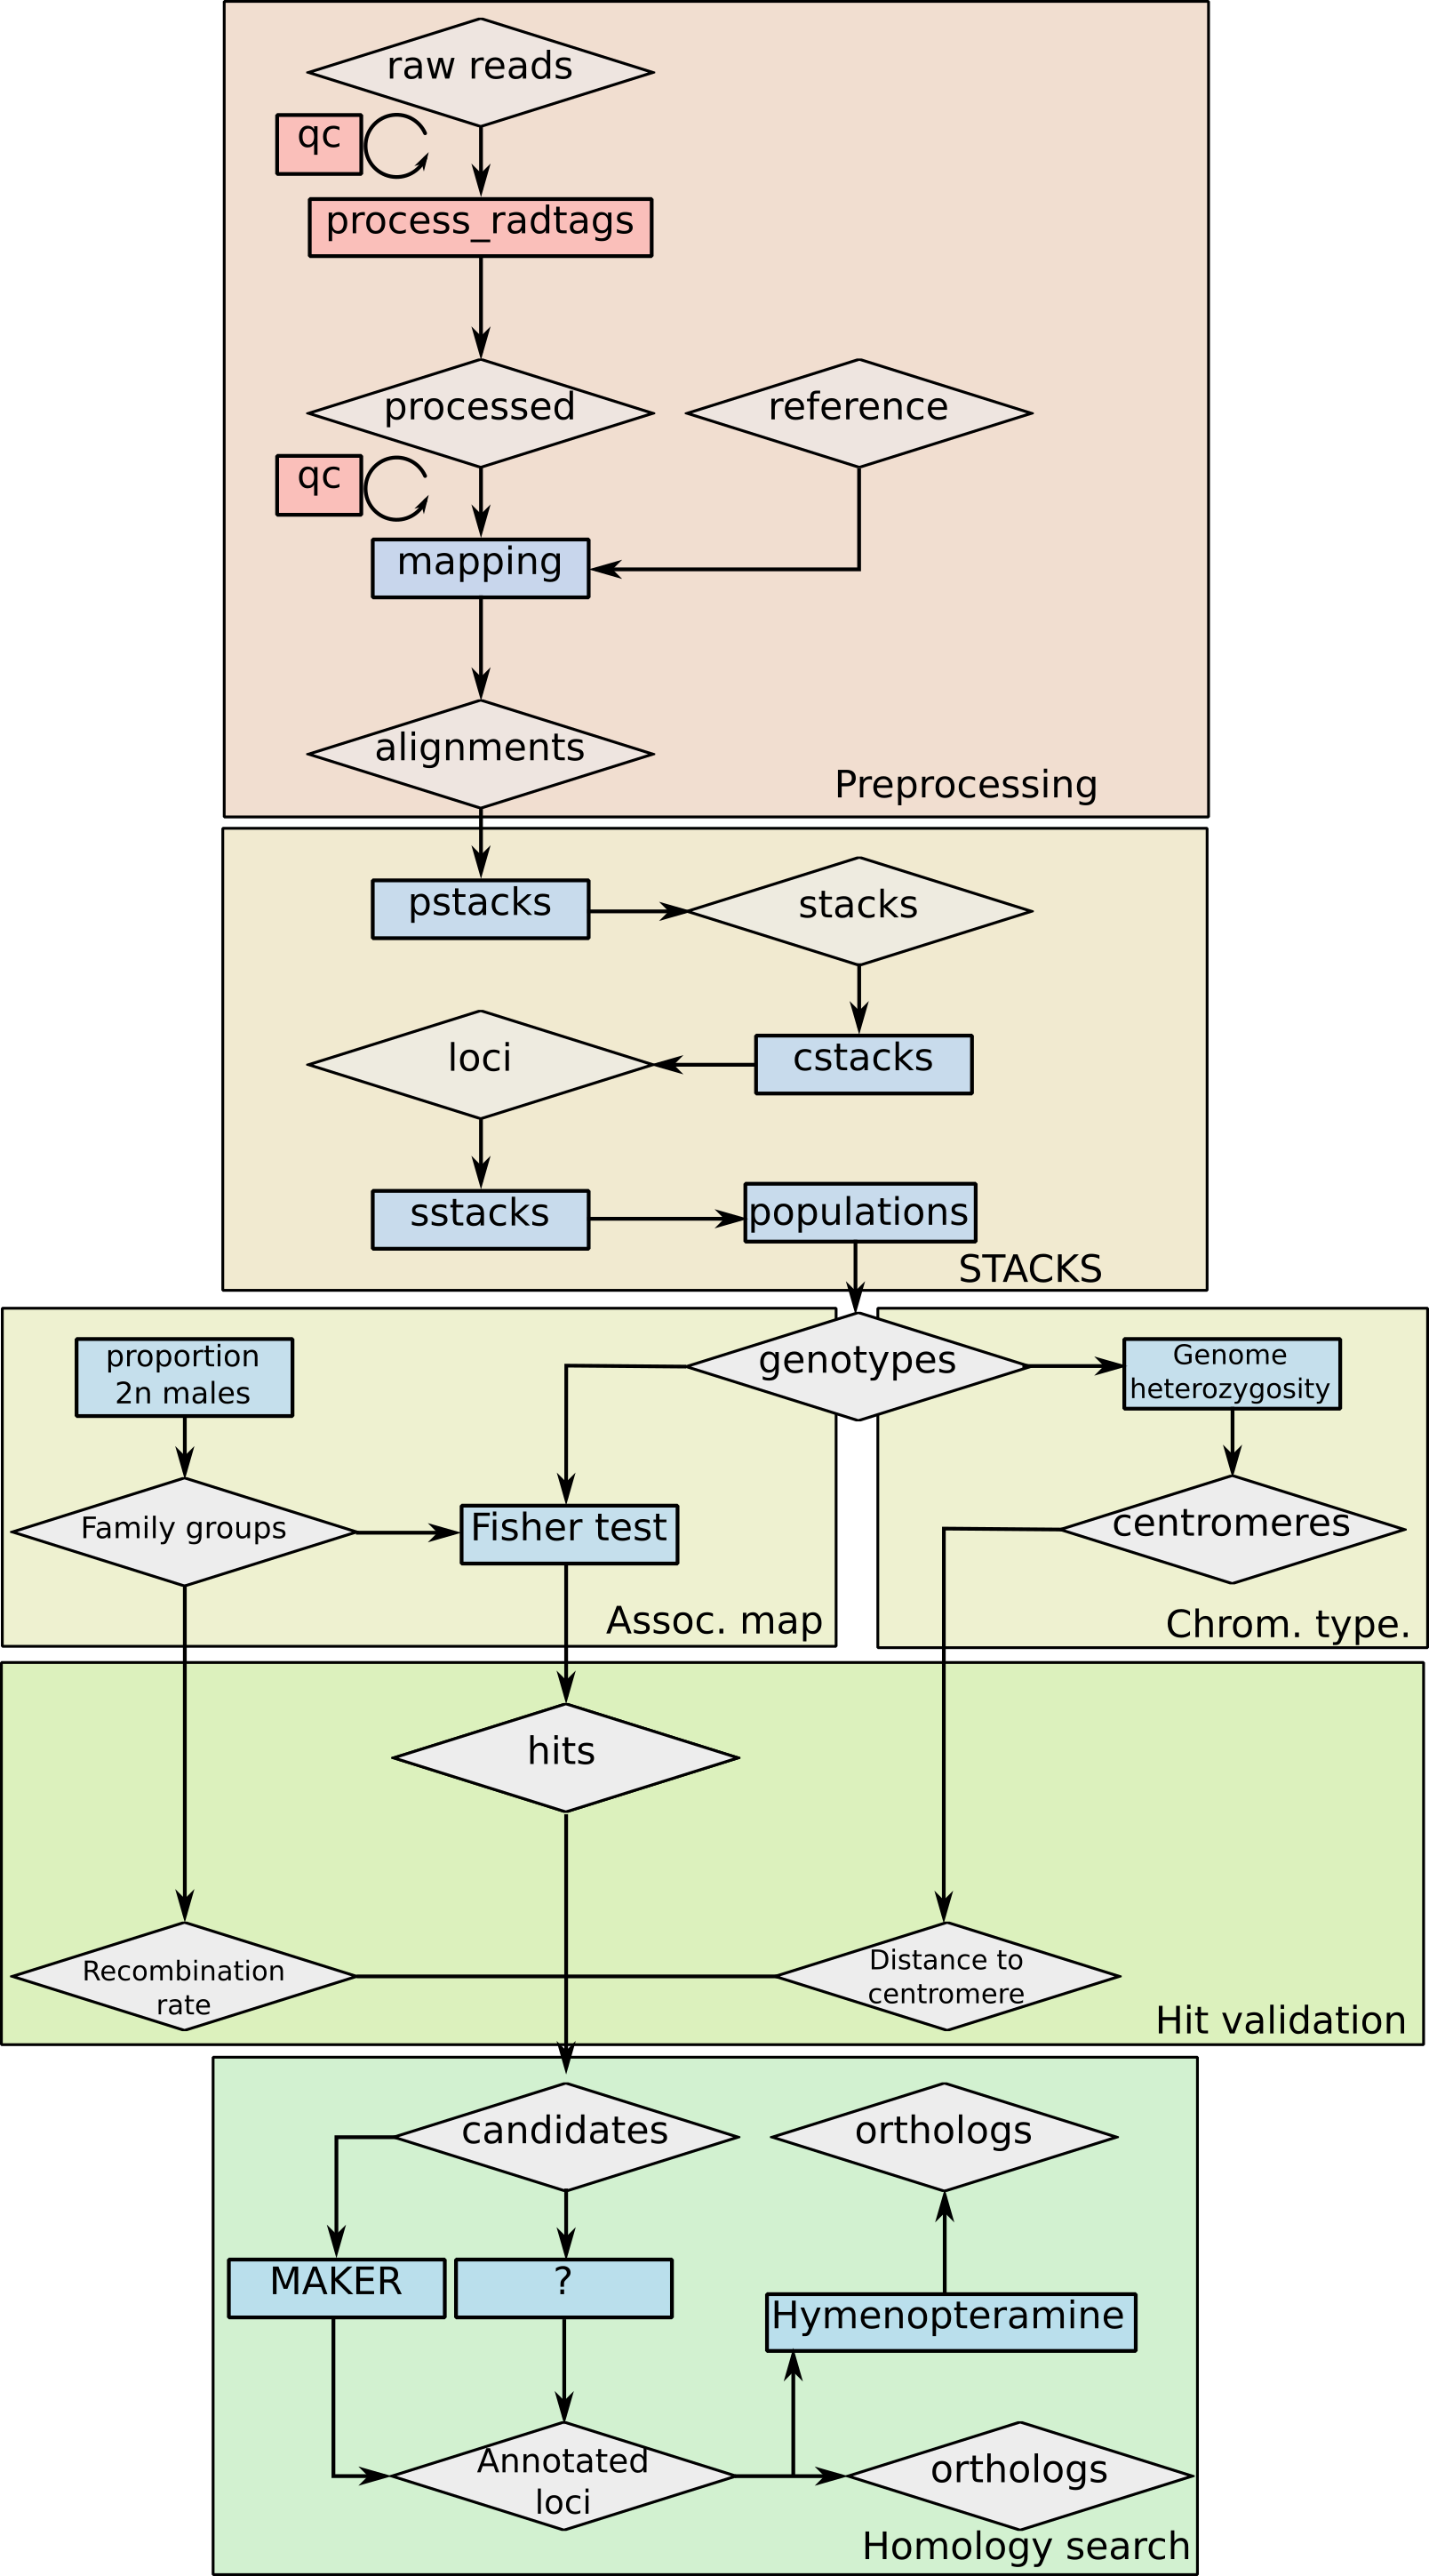
\includegraphics[scale=0.5]{flowchart}
\caption{\textbf{Pipeline described in the current lab book}. Diamonds represent data, rectangles represent operations/programs. Operations/programs in blue are included in the makefile, thos in red are not.}
\label{pipeline}
\end{figure}

 \chapter{Processing reads}
 RAD-seq data was split into 2 separate libraries: 7 and 7b. Together, the libraries contain 173 F4 individuals from 11 different F3 mothers. There were 96 samples in library 7 (one of which was contaminated) and 77 in library 7b. In total we have 172 valid samples across 11 families. Additionally, I inherited from 28 individuals from another library (lib6) which are offspring from families A and B.
 \section{Quality control}
 fastqc was used for quality control, separately on each file, and on all files together in the library.
 \section{Demultiplexing}
 The process-radtags program from stacks was used for demultiplexing and removal of Illumina adaptors. The operation was performed separately for libraries 7 and 7b:

\begin{lstlisting}
$ process_radtags -p raw/ -o processed/ -b \
/barcodes -e ecoRI --filter_illumina -E phred33 \
 -r -c -q --adapter_1 adapter --adapter_mm 2
\end{lstlisting}


\begin{center}
\begin{tabular}{c c}
lib7 & Truseq adapter, index 6 \footnotemark\\ 
lib7b & TruSeq adapter, index 12 \footnotemark\\
\end{tabular}
\end{center}
\footnotetext[1]{GATCGGAAGAGCACACGTCTGAACTCCAGTCACGCCAATATCTCGTATGCCGTCTTCTGCTTG}
\footnotetext[2]{GATCGGAAGAGCACACGTCTGAACTCCAGTCACCTTGTAATCTCGTATGCCGTCTTCTGCTTG}
\section{Trimming adaptors}
This step is performed by process radtags at the same time as demultiplexing. I tried different values for adapter mismatches, between 0 and 3 (i.e. reads containing sequences distant from the adapter by n mismatches are removed). This did not cause any major difference and therefore I will perform all downnstream analyses with an allowance of 2 mismatches in the adapter.

Note: Demultiplexing did not yield any read for CF4F10. 

\chapter{STACKS pipeline}

The pipeline described in this chapter will map the processed reads to the reference genome and build a catalogue of loci. It will eventually implement additional features such as calculating population statistics. At each step of the pipeline, I will try different combinations of parameters and choose the one yielding the best results. 

\section{Mapping}
Since the reference genome of \textit{Lysiphlebus fabarum} was recently released, I will first map the sequencing reads to the reference, using BWA, but I may also want to use bowtie to compare the results, eventually. At the moment, a draft reference genome is available, table \ref{assembly_stats} displays some summary statistics of it.
\begin{table}
\vspace{10px}
\csvautobooktabular[respect underscore=true]{stacks_pipeline/ref_genome_stats.csv}
\caption{Assembly statistics for the current reference genome of \textit{Lysiphlebus fabarum}}
\label{assembly_stats}
\vspace{10px}
\end{table}

\subsection{BWA}

BWA provides 3 different algorithms: MEM, backtrack (aln) and SW. MEM is normally the better for Illumina reads longer than 70bp, therefore I will be using this one here. Backtrack is preferred for short reads and SW with frequent gaps.
There are also 2 algorithms for building the index: 'is' and 'bwtsw'. 'is' is used with reference <2GB, 'bwtsw' with larger references.

General commands: 
\begin{lstlisting}
$ bwa index -p <out_index_name> -a <algorithm>
$ bwa mem <index> <sample.fq> > <out.sai>
> $sample-$prefix.sam
\end{lstlisting}

When using bwa-aln, there the command running the alignment (after indexing) is:
\begin{lstlisting}
$ bwa aln -n <mismatches> $index <sample.fq> > <sample.sai>
$ bwa samse -n <max_dupl> $index $sample.sai $data_dir/$sample.fq.gz
\end{lstlisting}
The first command (bwa index) constructs an index from the reference genome, whereas the second one (bwa mem/aln) actually runs the aligner. The third command (bwa samse) allows to transform the .sai into .sam files.

Here is the list of different mapping parameters I may try with bwa-mem:
\begin{itemize}
\item -k : minimum seed length (will miss matches shorter than value)[19]
\item -w : band width (gaps longer than value will not be found)[100]
\item -d : maximum distance between query and reference positions before stopping seed extension. [100]
\item -r : triggers reseeding for a MEM longer than min\_seed\_len$*$float. Larger values yield fewer seeds $->$ faster alignment but lower accuracy [1.5].
\end{itemize}

In the case we use the backtrack (aln) algorithm instead of MEM, the only parameter worth tuning is -n, the number of mismatches allowed. 


Note: I did not include parameters that are not relevant to sensitivity (e.g. threads) or parameters that involve scoring (changing these naively would probably have a negative impact). Full list of parameters is on the \href{http://bio-bwa.sourceforge.net/bwa.shtml}{official bwa website}

Note2: About multiple hits and BWA-mem: 

(https://github.com/lh3/bwa)

2. Why does a read appear multiple times in the output SAM?

BWA-SW and BWA-MEM perform local alignments. If there is a translocation, a gene fusion or a long deletion, a read bridging the break point may have two hits, occupying two lines in the SAM output. With the default setting of BWA-MEM, one and only one line is primary and is soft clipped; other lines are tagged with 0x800 SAM flag (supplementary alignment) and are hard clipped.


\subsection{Bowtie2}
General commands: 
\begin{lstlisting}
$ bowtie2-build reference_genome.fa L_fabarum
$ bowtie2 -x <ref_index> -U <unpaired_reads_files> -S <out_SAM_file>
\end{lstlisting}
The first command (bowtie2-build) constructs a set of index (extension: .bt2) from the reference genome, whereas the second one actually runs the aligner.

Here is the list of different mapping parameters I may try:
\begin{itemize}
\item --trim5 <n> : trim n bases from the 5' end (left) of each read before alignment
\item --trim3 <n> : trim n bases from the 3' end (right) of each read before alignment
\item -D : maximum number of seed extension that can fail in a row before stopping (increasing makes bt2 slower)
\item -R : maximum number of re-seeding when attempting to align read with repetitive seeds (increasing makes bt2 slower)
\item -N : number of mismatches permitted per seed (increasing reduces false negative, but makes bt2 slower)
\item -L : length of seeds (decreasing makes bt2 slower but more sensitive)
\item -i : interval between seeds (increasing makes bt2 slower but more sensitive)
\end{itemize}

Recommandations from the bowtie2 website to make alignment more sensitive: 
a) make seeds closer (reduce i)
b) make seeds shorted (reduce L)
c) allow more mismatches per seed

End-to-end versus local alignment (--local): end to end takes all bases in the reads into account, while local allows to trim reads to exclude the ends from the alignment.
Seeds are substring of the reads which bowtie2 tries to align to narrow down the valid regions for aligning a read. There is a list of preset values for these parameters on the \href{http://bowtie-bio.sourceforge.net/bowtie2/manual.shtml#preset-options-in---end-to-end-mode}{official bowtie2 website}. Preset parameters differ between local and end-to-end modes.
There are other parameters, such as score weights for gaps mismatches and allowance for 'N' ambiguous characters but changing these naively could probably have negative effect on the alignments.
Procedure: try out different preset values and select the one yielding the best results. Then, eventually tweak the parameters slightly from the preset values. These simulations can be run on a subset of individuals to speed up the process.

note to self: at the end of a run, bowtie2 prints a summary to stderr such as:

20000 reads; of these:

  20000 (100.00\%) were unpaired; of these:
  
    1247 (6.24\%) aligned 0 times
    
    18739 (93.69\%) aligned exactly 1 time
    
    14 (0.07\%) aligned $>$1 times
    
93.77\% overall alignment rate
\vspace{10px}\\
If I use Bowtie2, I will redirect the stderr and parse it into a csv file and generate plot to visually estimate the best parameter values.

\subsection{Mapping results}

I used the aln algorith of bwa, since the mem algorithm did not report multiple alignments and has very few documentation available. I tried different mismatches values with aln (Figure \ref{map_results}), ranging from 0 to 8, and I chose to use 4 since the increase in single was quite low above this value. When the mismatch parameter is set to 4, running bwa-aln on a subset of 12 samples yielded 57\% of single hit reads, 26\% of multiple hits and 17\% of unmapped reads.

\begin{figure}[h]
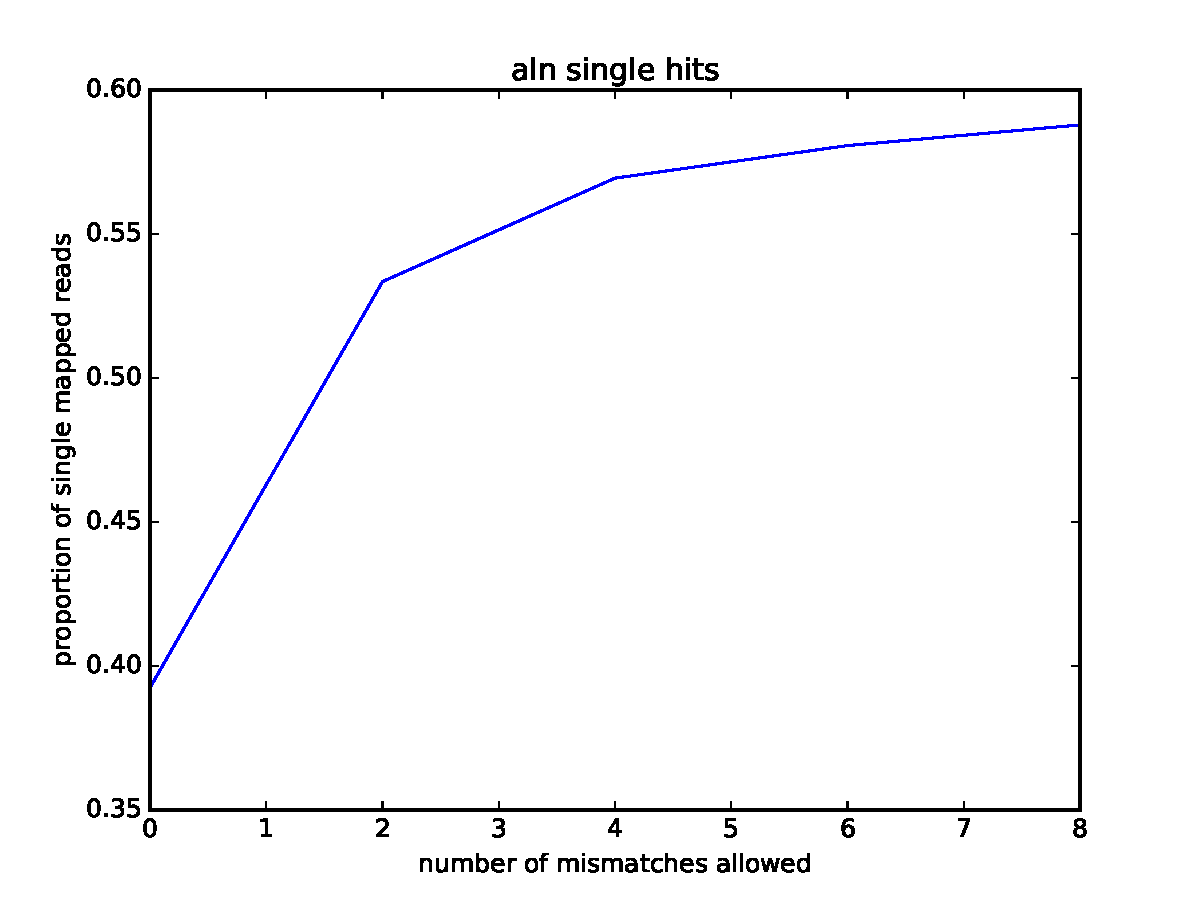
\includegraphics[scale=0.5]{param_space/mapstats}
\caption{Results of the BWA mapping with different parameter values for the number of mismatches allowed during mapping. The plot shows the proportion of reads that are mapped uniquely to the reference genome.}
\label{map_results}
\end{figure}

\section{pstacks}

pstacks is a component of the STACKS suite that takes stacks of reads aligned to a reference genome as an input (typically in the SAM format) and idenify SNPs

general command: 
\begin{lstlisting}
$ pstacks -f <input_path> -i <sample_ID_int> -o <out_dir> \
 -m <min_depth> -p <num_threads> -t <file_type>
\end{lstlisting}

Parameters I may want to change are: 
\begin{itemize}
\item -m : minimum depth of coverage required to call a stack [3]
\item --max\_clippped : alignments with more than X soft-clipped bases are discarded [15\%]
\item --min\_mapq : minimum required quality [10]
\end{itemize}

Note: there are 3 models; SNP, bounded SNP and fixed. SNP is the default model, bounded SNPs allows to give prior expectations about the error rate, which can allow better estimations of heterozygosity and the fixed model identifies all fixed sites and masks all others.

\subsection{pstacks results}

Pstacks was run on aligned reads (BWA, 4 mismatches allowed). I tried different values for the minimum coverage required to call a stack (-m parameter), ranging from 1 to 6 (Figure \ref{pstacks_param}). Below is the value for minimum coverage, along with the mean number of loci and alleles that was produced per sample. This table was produced including all non-empty samples (198 individuals) and the variables are averaged (arithmetic mean) over all those samples.

\begin{table}
\begin{center}
\vspace{10px}
\csvautobooktabular[respect underscore=true]{param_space/pstats.csv}
\vspace{10px}
\caption{Summary statistics of stacks obtained with different parameter values for minimum coverage in pstacks.}
\label{pstacks_param}
\end{center}
\end{table}

I will use 4 reads minimum coverage as this is already high and using lower values does not improve the output in anyway.

Note: Locus are regions formed by one or more stacks. Alleles are different stacks at the same locus.

\section{cstacks}

cstacks is a component of the STACKS suite that builds a catalog of loci with different alleles from a set of processed samples.

general command: 
\begin{lstlisting}
$ cstacks -s <sample_prefix> -o <out_dir> -b <catalogue_ID>\
-p <num_threads> -n <num_mm> -M <pop_map>
\end{lstlisting}

Parameters I may want to change are: 
\begin{itemize}
\item -n : Number of mismatches allowed between sample loci when building catalogue [1]
\item -g : base catalog on alignment position instead of sequence identity
\end{itemize}

Note: There are also advanced options such as gapped assembly parameters and loci matching multiple catalogue entries, but these are probably not relevant here.
\subsection{cstacks results}

I changed the number of mismatches allowed between samples between 1 and 4. Table \ref{cstacks_param} shows the results with a subset of 11 samples $([A-L\&\&[\wedge B]]01)$ because B01 was empty (few, low quality reads). 

\begin{table}
\begin{center}
\vspace{10px}
\csvautobooktabular[respect underscore=true]{param_space/cstats.csv}
\vspace{10px}
\caption{Summary statistics of loci obtained with different parameter values in cstacks.}
\label{cstacks_param}
\end{center}
\end{table}

I tried running cstacks on all (non-empty) samples, and also modifying the script so that it will first compute the mean number of tags (reads) across all samples, and exclude those with less than 10\% of this value when building the catalogue. From the 202 original samples, 4 were empty and excluding low quality ones removed 13 additional ones.\\

Update: 21.07.2017\\
When including mothers, I reach a total of 212 individuals. I use the same filtering strategy to exclude samples with low amounts of reads (Figure \ref{tags_dist}). From the 212 original samples, I excluded 17 low quality samples, among which 4 were totally empty.

\begin{figure}[h]
	\begin{center}
		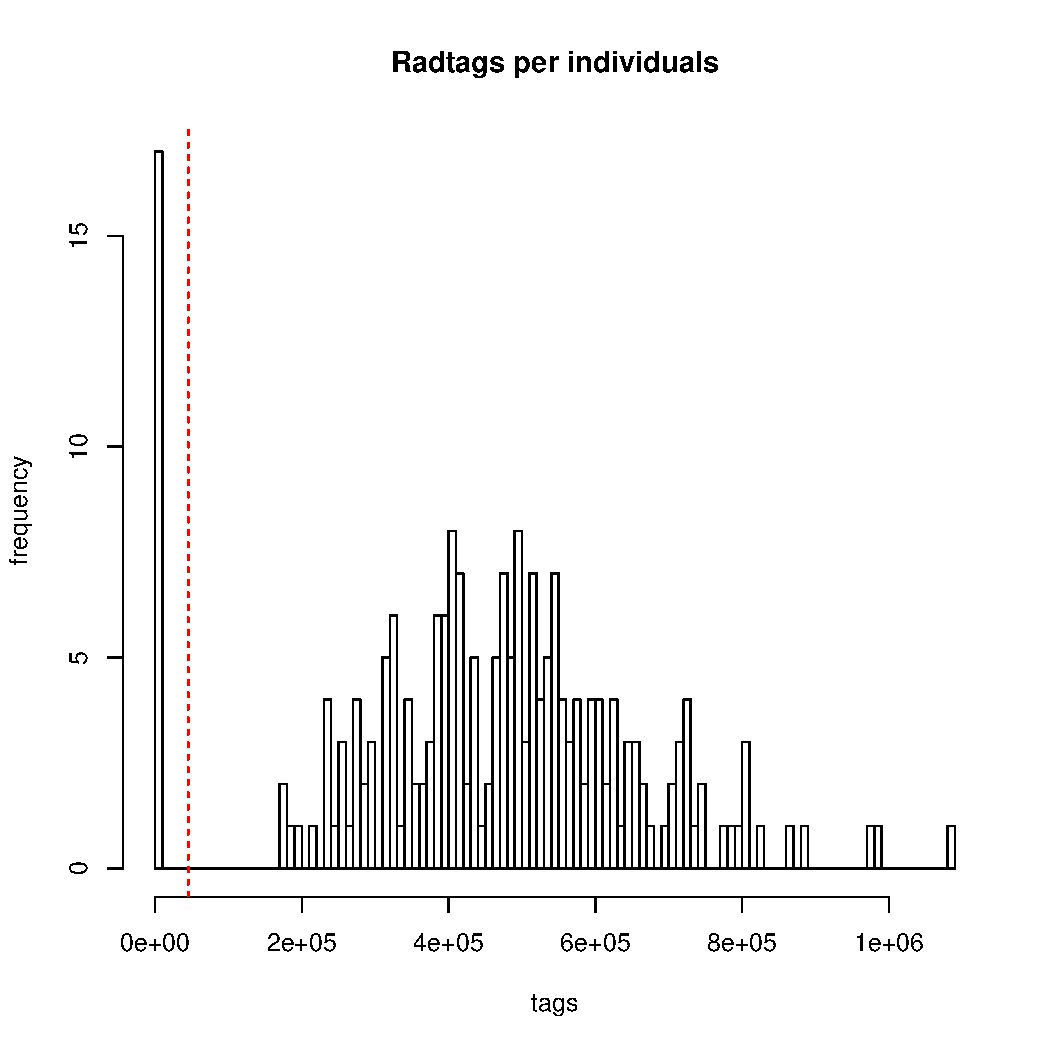
\includegraphics[width=0.7\textwidth]{stacks_pipeline/radtags_distrib.pdf}
		\caption{distribution of the number of radtags (reads) per sample. The red vertical dashed line indicates the cutoff value set to 10\% of the mean. Samples below this value are removed from the analysis.}
		\label{tags_dist}
	\end{center}
\end{figure}
\FloatBarrier
Summary results with n=1:
\begin{itemize}
\item All non-empty samples (198): 25618 alleles in catalogue, over 7062 loci.
\item Excluding samples with \textless 10\% of mean tags (185): 25585 alleles in catalogue, over 7046 loci
\end{itemize}

note: following recommandations from Paris et al. 2017, Lost in parameter space: a roadmap for STACKS. \textit{Methods in Ecology and Evolution}, I set the value of n to 3 (M-1=3)

\section{sstacks}

sstacks is used to generate one file per individual, in each file, the matching loci point to the cstacks catalogue. There is no crucial parameter to change in this program.

\section{populations}

The "populations" component of STACKS is used to compute population genetics statistics on a set of individuals. I use it here to compute FST statistics (fixation index) along the genome. It offers several features to compute different statistics, including a bootstrapping feature and a "kernel smoothing" flag, allowing to take neighbouring region into account with a decreasing weight as a function of their distance from the focus nucleotide. I will use both of these features to compute FST.

The main features to change in FST calculation are :
\begin{itemize}
\item -r: minimum percentage of individuals in a population required to process a locus for that population.
\item -p: minimum number of populations a locus must be present in to be procesed.
\item -m: minimum stack depth required for individuals at a locus.
\end{itemize}

Example populations call for FST calculation:
\begin{lstlisting}
$ populations -P <stacks_files> -M <popmap> -b 1
 -k -r 0.75 -f p_value
\end{lstlisting}

\subsection{populations results}

I ran populations with the following parameters:
\begin{itemize}
\item -r: 0.75 - 0.85
\item -p: 2
\item -m: 5
\end{itemize}

Therefore, only loci with at least 5 reads of coverage were included, each loci also needs to be in at least 75\% to 85\% of all individuals and in both populations (males and females).

This table summarizes the first statistics I extracted from the VCF files (using vcftools) with the different values for r:
\begin{center}
\vspace{10px}
\csvautobooktabular[respect underscore=true]{param_space/vcf_sumtable.csv}
\vspace{10px}
\end{center}

plotting the inbreeding coefficient per individual with r=75 yields:

\begin{figure}[h]
	\begin{center}
		\hspace*{-1in}
		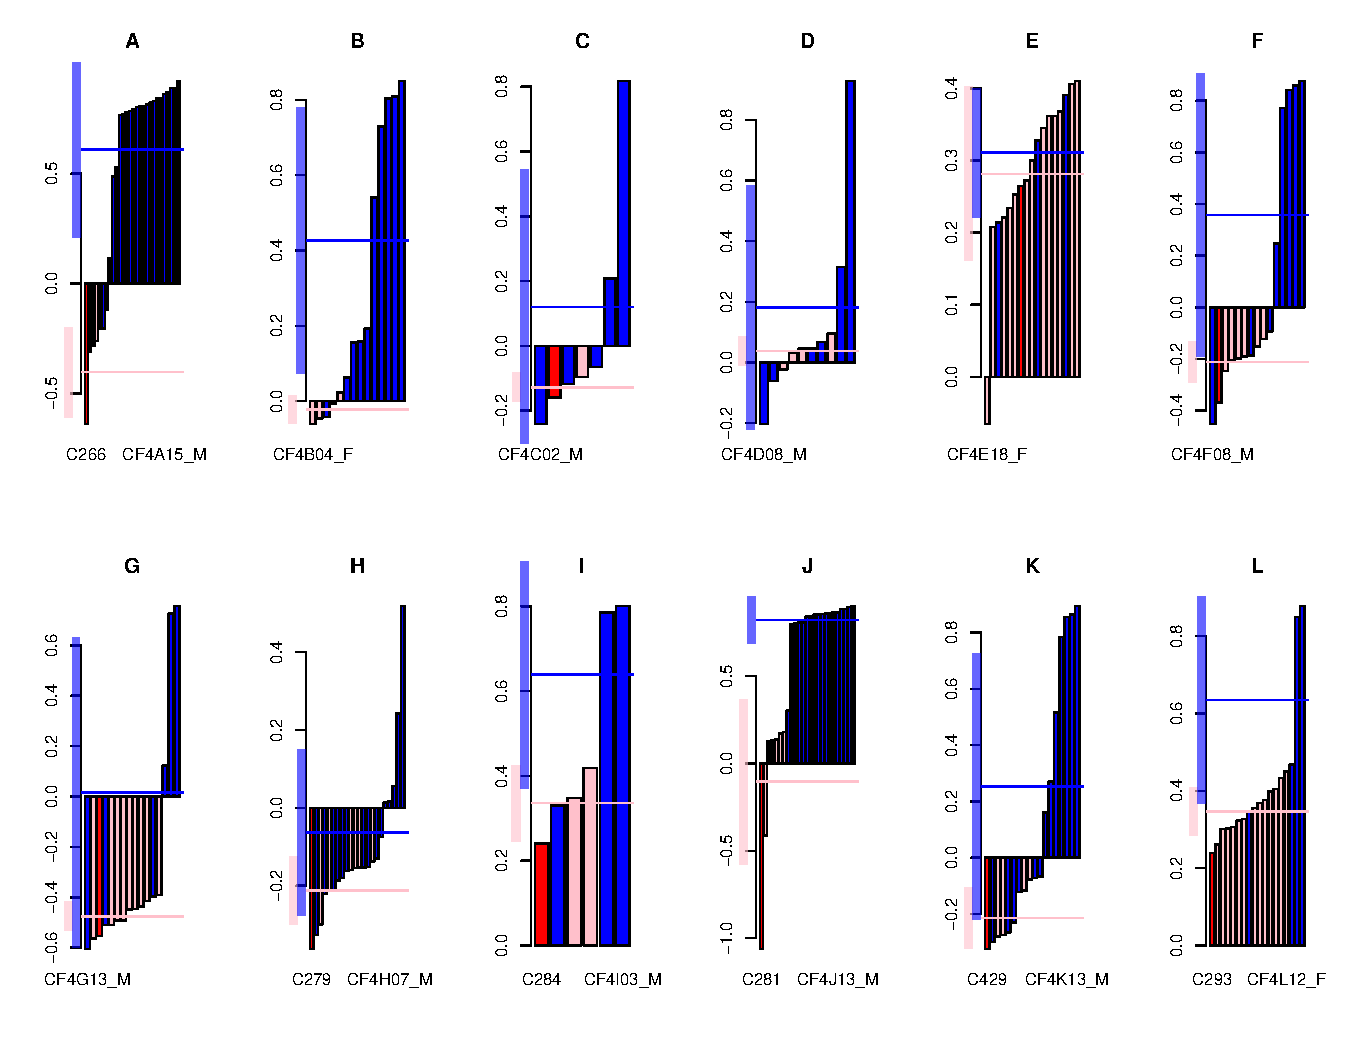
\includegraphics[width=1.5\textwidth]{F_d-25_r-75}
		\caption{Inbreeding coefficient (F). Each plot is a family, each bar is an individual. Blue bars represent males and pink ones represent females and red ones are mothers. color bars on the y axis span the mean +- standard deviation of males and females, respectively. In theory, mothers should have the lowest inbreeding coefficient of their family (highest heterozygosity)}
	\end{center}
\end{figure}

When increasing the minimum depth above ~15, populations crashed. Disabling bootsrapping and kernel smoothing fixed the issue. Guess: May be caused by a contig smaller than the sliding window size during kernel smoothing. This could be the case if the sliding window has a min number of loci, in which case increasing minimum depth would cause the window to enlarge.

I tested for correlations between Mean depth of loci and homozygosity in all individuals and per family, no significant correlation was found. This means there should not be significant allele excludion caused by too stringent min depth (i.e. stacks removed because of low coverage, resulting in homozygous loci).

\section{STACKS parameters summary}
\begin{table}[h!]
\begin{tabular}{c|c}
process radtags & Mis:2\\
bwa & Mis:4\\
Pstacks & MinDep:3\\
Cstacks & LocMis:1\\
Sstacks & -\\
populations & IndProp:0.75, MinDep:5(25)*, MaxHet:0.9\\
\vspace{5px}
\end{tabular}
\\
 \footnotesize * Stringent MinDepth value used to exclude haploid males. The smaller value is used for downstream analyses to keep more loci.
\end{table}

\FloatBarrier

\chapter{Excluding haploids}

I used the F statistics (coefficient of inbreeding) computed by vcftools to measure homozygosity levels in each individual. The F statistics used were generated with more stringent parameters (min depth: 25) to call ploidy more confidently. It is calculated as $F = \frac{O-E}{N-E}$ where O is the observed number of homozygous loci, E is the number expected by chance and N is the total number of loci.

First, I calculated the Mean $\mu$ and standard deviation $\sigma$ of the inbreeding coefficient $F$ among daughters in each family. I then classified males with:
\\
\begin{center}
 $F > \mu + 2\sigma $  \\
\end{center}

 as haploid. This is stringent threshold should exclude all haploid males, but it can also potentially exclude diploid males from the analysis.

Update: 08.06.2017

I tried 12 different thresholds for excluding haploids. The thresholds were computed according to these rules:
\begin{itemize}
\item 1: All thresholds follow the formula $\mu + \tau(N\sigma)$ with $1 \leq N \leq 4$
\item 2:  $1 \leq \mu \leq 4$
\item 3: $\tau$ is a function for transforming the inbreeding coefficient values. Either $\tau(F) = F^2$ or $\tau(F) = \sqrt{F}$
\end{itemize}
As shown above, in this report I will use the threshold named "m2" which corresponds to  $F > \mu + 2\sigma $.
Figure \ref{haplodiplo} shows a plot showing the separation of haploid and diploids using this threshold.

\begin{figure}[h]
	\begin{center}
		\hspace*{-0.8in}
		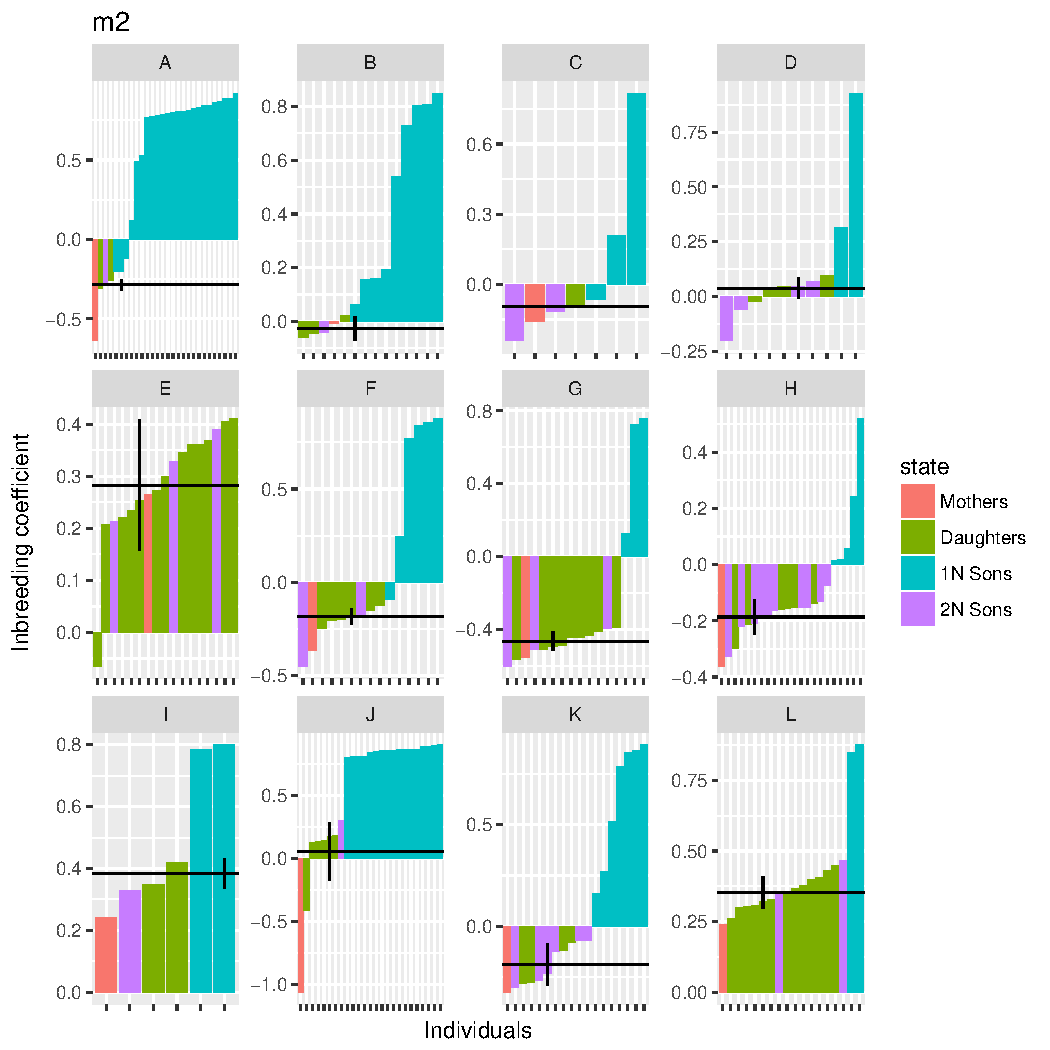
\includegraphics[width=1.2\textwidth]{exclu_haplo/m2}
		
		\caption{Inbreeding coefficient (F). Different colors represent the different types of individuals, as shown in the legend. Each plot is a family, each bar is an individual. Horizontal black bars show the mean inbreeding coefficient of daughters within the family $+/-$ the standard deviation (vertical black line). In theory, mothers should have the lowest inbreeding coefficient of their family (highest heterozygosity)}
		\label{haplodiplo}
	\end{center}
\end{figure}

\FloatBarrier

After separating haploids from diploids, I performed exploratory analyses prior to association mapping. The goal of these is to assess the homozygosity rate of SNPs in diploid males and females and how many seem to fit the CSD pattern. As shown in Figure \ref{SNPs_explo5} and \ref{SNPs_explo25}, there is no single SNPs thatis heterozygous in all females and homozygous in all diploid males. That can imply that the species has ml-CSD and there is no single locus that always fit the CSD pattern, or the restriction enzyme used in the RAD-seq protocol (ecoR1) did not cut in the CSD locus directly. It is very likely a combination of both explanations. It is also worth mentioning that, besides the number of SNPs, it makes little difference whether I use permissive (Figure \ref{SNPs_explo5}) or stringent (Figure \ref{SNPs_explo25}) parameters. The only notable change is that including more SNPs results in higher homozygosity for both sexes.

In this analysis, I excluded all consensus loci (where all individuals had the same allele) and did not consider SNPs with more than 2 genotypes in a single individuals in the heterozygosity calculation (counted as missing values), as they are likely due to contaminations.

\begin{figure}[h]
	\begin{center}
		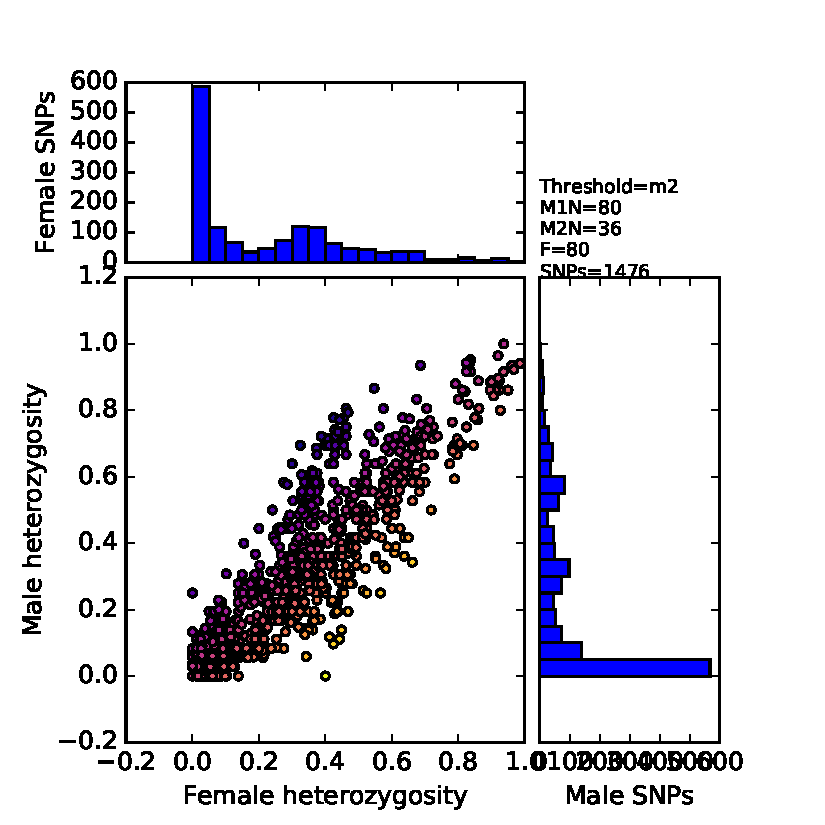
\includegraphics[width=0.8\textwidth]{exclu_haplo/d5assoc_explo/m2}
		\caption{Homozygosity of female and diploid male SNPs where depth $\geq 5$ (permissive parameters). Each point on the scatterplot is a SNP, and its coordinate are the proportion of females (x) and males (y) in which it is homozygous. Histograms allow to visualize the distribution of homozygosity for SNPs of each sex. The color code shows how SNPs fit the CSD pattern with lighter points being closer to it (i.e. more homozygous in males and heterozygous in females). Summary statistics on the top right show the threshold used, the number of haploid males excluded (M1N) as well as the number of diploid males (M2N), females (F) and SNPs included.}
		\label{SNPs_explo5}
	\end{center}
\end{figure}

\begin{figure}[h]
	\begin{center}
		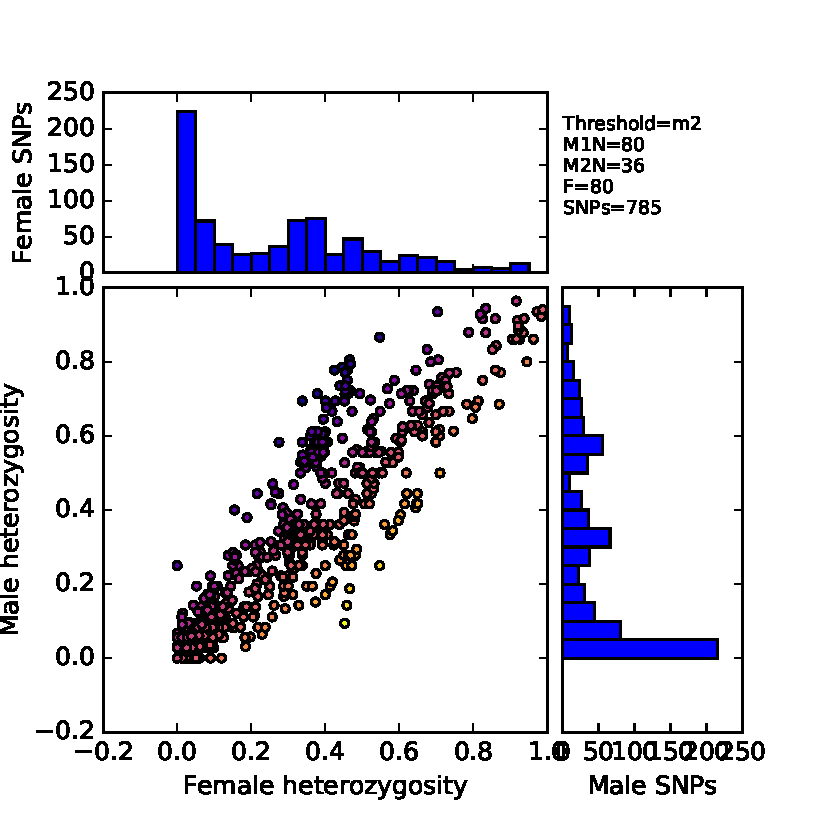
\includegraphics[width=0.8\textwidth]{exclu_haplo/d25assoc_explo/m2}
		\caption{Homozygosity of female and diploid male SNPs $\geq 25$ (stringent parameters). Each point on the scatterplot is a SNP, and its coordinate are the proportion of females (x) and males (y) in which it is homozygous. Histograms allow to visualize the distribution of homozygosity for SNPs of each sex. The color code shows how SNPs fit the CSD pattern with lighter points being closer to it (i.e. more homozygous in males and heterozygous in females). Summary statistics on the top right show the threshold used, the number of haploid males excluded (M1N) as well as the number of diploid males (M2N), females (F) and SNPs included.}
		\label{SNPs_explo25}
	\end{center}
\end{figure}


\FloatBarrier

\chapter{Cleaning genomic data}

date : 23.06.2017
\\

The first attempt at separating individuals based on inbreeding coefficient revealed several issues inherent to the data:
\begin{itemize}
\item The inbreeding coefficient is not clearly bimodal in all families (1 haploid mode and 1 diploid mode)
\item Some loci have more than 2 haplotypes, although we are working with diploids.
\item There are no loci that clearly stand out as perfectly 'CSD like' among all individuals, this should be looked at family-wise.
\end{itemize}
These issues will be solved one by one in this chapter.

\section{Improving ploidy separation metric}

The inbreeding coefficient was computed using all males/females. Also, the raw heterozygosity may be a more accurate metric than inbreeding coefficient. Both issue require the analysis to be done in a per-family fashion, either by re-running the populations program for each family, or implementing family as an additional population layer.
\\
Date: 27.06.2017
\\
Solution: I could switch to observed homozygosity, but I think it is also fine to keep this metric (I can always change it later). I did however, re-run the populations program separately for each family. I did not add a population layer to the popmap, because it would not have allowed for different loci blacklists between families when solving the third issue. Visualizing the distribution of inbreeding coefficients across individuals reveals a pretty good (?) separation of individuals (Figure \ref{ploidy_metric}).


\begin{figure}[h]
	\begin{center}
		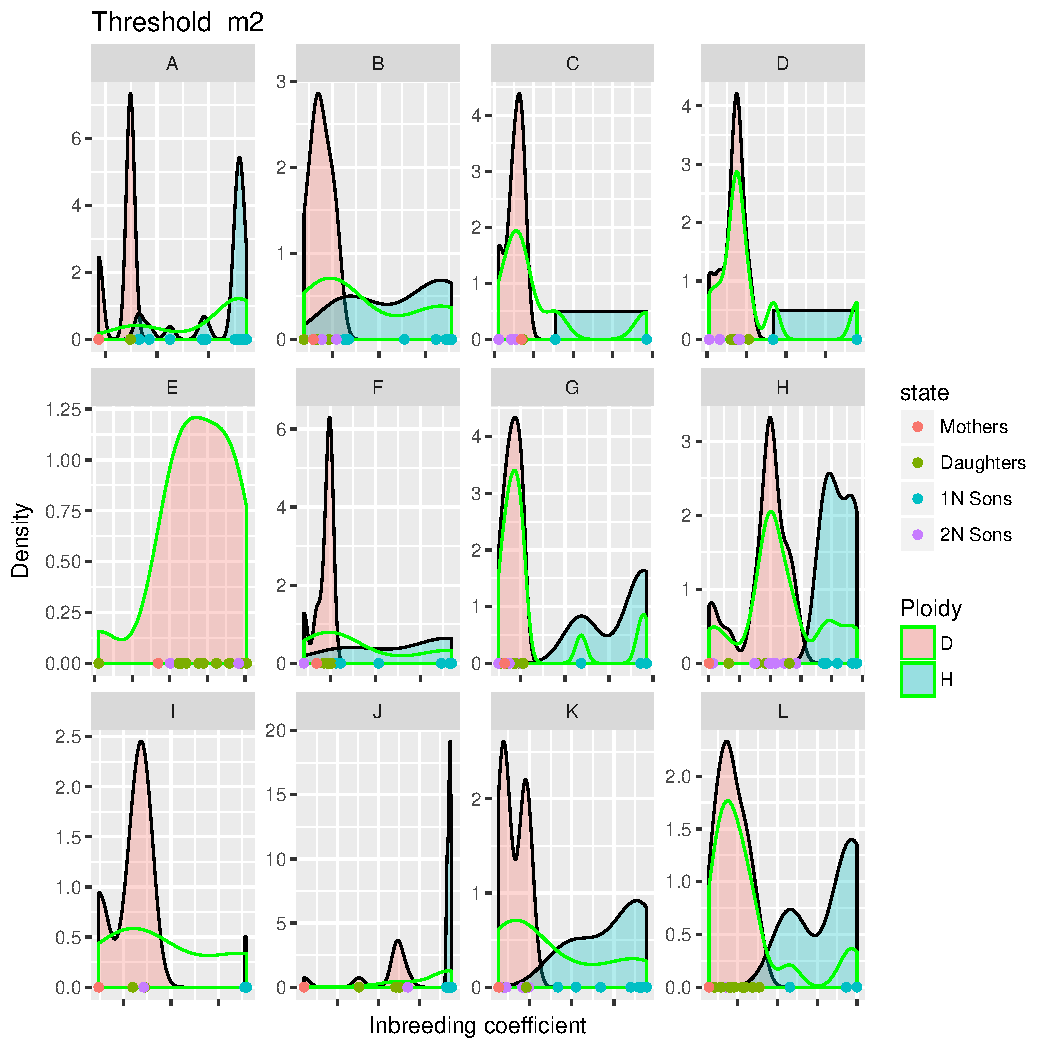
\includegraphics[width=0.8\textwidth]{cleaning_genomic_data/F_r-75_d-5_m2_density.pdf}
		\caption{Distriution of individual inbreeding coefficient. The green curve represents the overall distribution of inbreeding coefficients within the family. The blue and pink areas represent the distribution of inbreeding coefficients for haploids and diploids, respectively, split using the m2 threshold defined at the beginning of chapter 4. Ideally, the green curve would follow a bimodal distribution clearly separating individuals by homozygosity.}
		\label{ploidy_metric}
	\end{center}
\end{figure}

Date: 12.07.2017
Update: This method of ploidy separation is flawed as it will overestimate the number of haploid males in families with few females. Indeed, with a lower standard deviation of female homozygosity, the threshold tends to the mean only.

Because the homozygosity of diploid offspring depends on its mother, but that of haploids are independent of mother background, I can probably use a universal threshold for all families. This way, the threshold can be equally conservative in all families and not biased towards certain of them. Plotting homozygosity of all individuals (Figure \ref{ploidy_fixed}) revealed 2 separate meta-distributtions. The one on the left is a gaussian made up of several smaller ones (each smaller distribution is a family, with the mean depending on the mother), whereas the distribution on the right is made of a single gaussian containing all (or most) haploid males.
Choosing a fixed conservative threshold in between should allow to keep more individuals and remove bias.

\begin{figure}[h]
	\begin{center}
		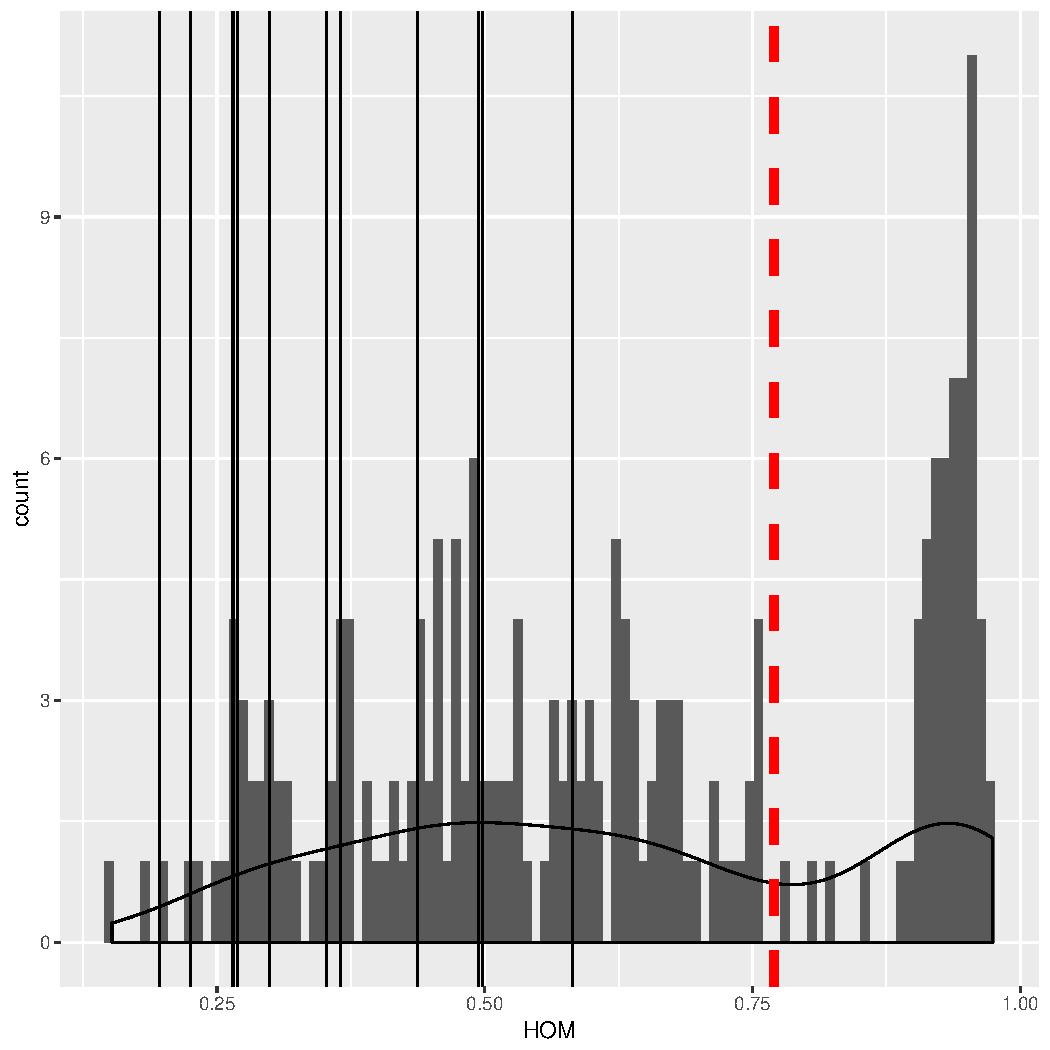
\includegraphics[width=0.8\textwidth]{cleaning_genomic_data/ploidy_sep_fixed.pdf}
		\caption{Distribution of the proportion of homozygous loci across all individuals. Continuous vertical black lines are the mothers values and the dashed vertical red line is the (visually) optimal threshold, fixed at 0.77.}
		\label{ploidy_fixed}
	\end{center}
\end{figure}

\section{Loci with 3 or more haplotypes}

There are two possible explanation for the existence of these loci. It could be either due to a contamination, in which case few individuals would present many loci with 3 or more haplotype. On the other hand, if few loci have this issue in several individuals, it could be due to paralog merging. This can be solved by identifying which case is the most likely, and either excluding concerned individuals (first case), or loci (second case).

24.06.2017: Asked on STACKS google group about the haplotypes.tsv file. It is apparently normal to have more than 2 genotypes and depends on the parameters that were set in pstacks/ustacks. The answer I got, is that I should only work with the VCF file, which calls only 2 genotypes/site/individual. This imply figures \ref{SNPs_explo25} and \ref{SNPs_explo5} are not valid, as I misinterpreted the file content. I will re-generate these figures using the VCF file directly.
\\
Date: 27.06.2017
\\
Solution: I used the -012 argument in VCFtools to produce a genotype matrix from the populations output VCF file. This matrix encodes the genotype of each individual at each SNP with an integer representing the number of non-reference alleles present. These matrices were generated separately for each family and used to regenerate the figures \ref{SNPs_explo25} and \ref{SNPs_explo5}.

The issue when visualizing the SNPs heterozygosity per family (Figure \ref{SNPs_explo_fam}) is that the low number of individuals allow for few different heterozygosity values for any given SNPs, yielding a high number of 'perfectly' CSD-like candidates. Solving the next issue or grouping SNPs by contig/locus may help reduce this number, but ultimately only association mapping will allow to find the best candidate region. 


\begin{figure}[h]
	\begin{center}
		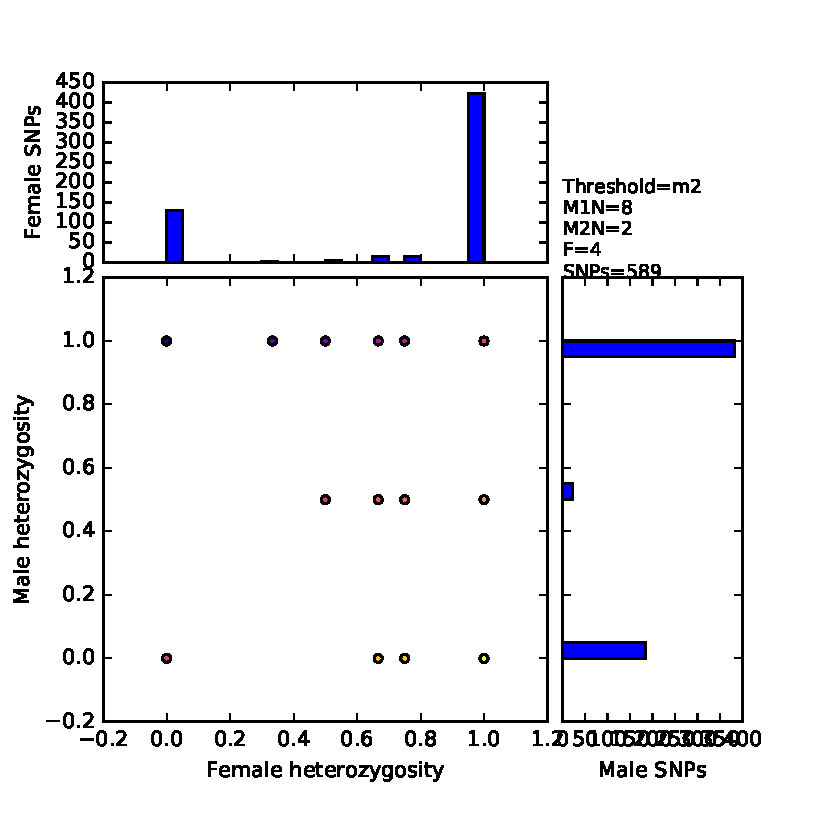
\includegraphics[width=0.8\textwidth]{cleaning_genomic_data/assoc_explo_fam/B.pdf}
		\caption{Example: SNPs heterozygosity across individuals of family B. The yellowness represents the proximity to CSD-like pattern (i.e. homozygous in all males and heterozygous in all females. Note: populations parameters set to : min depth (D)=5 and prop pop (r)=75}
		\label{SNPs_explo_fam}
	\end{center}
\end{figure}


\section{No clear signal in whole population}

This issue could be expected from the biological system because it is believed that there is ml-CSD in this species; there should be no single locus that will fit the CSD pattern across all individuals. This mean we need to identify different loci independently in each family. There are several things which can be done to work around this issue. 

First, and most importantly, the populations program should be taking family information into account, but this was done already when solving the first issue (Improving ploidy separation metric). Second, the data should be cleaned by blacklisting loci that are homozygous in mothers in each family, as there is no way these will be heterozygous in their respective daughters and be CSD candidates.
\\
Date: 29.06.2017
\\
Solution: I re-ran the explo assoc script used to generate figure \ref{SNPs_explo_fam} and excluded all SNPs that are homozygous in the mother (Figure \ref{SNPs_explo_nomother}). It removed a significant number of SNPs from the set, but there are still way too many that fit the CSD pattern.

\begin{table}
	\begin{center}
		\csvautobooktabular[respect underscore=true]{cleaning_genomic_data/hom_mother.txt}
		\caption{Number of homozygous SNPs found in the mother of each family. Note family D is excluded since there was no genomic data available for this mother.}
		\label{hom_mother}
	\end{center}
\end{table}

\begin{table}
	\begin{center}
		\csvautobooktabular[respect underscore=true]{cleaning_genomic_data/CSD_like.txt}
		\caption{Number of homozygous SNPs that fit the CSD pattern in each family.}
		\label{CSD_like_raw}
	\end{center}
\end{table}


\begin{figure}[h]
	\begin{center}
		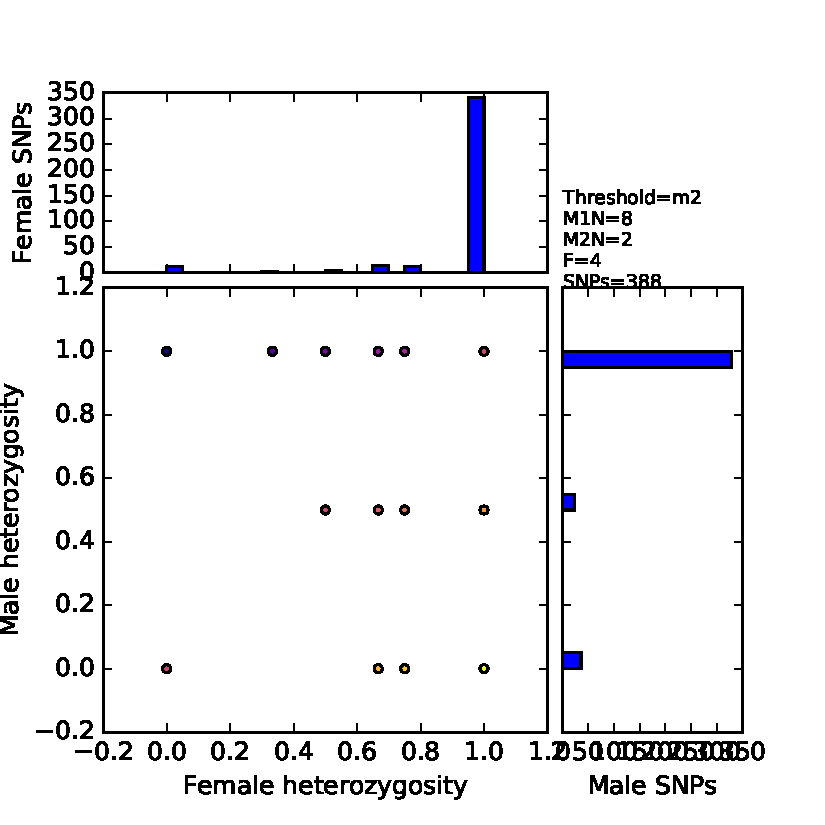
\includegraphics[width=0.8\textwidth]{cleaning_genomic_data/assoc_explo_fam_no_mother/B.pdf}
		\caption{Example: SNPs heterozygosity across individuals of family B after removing SNPs that are homozygous in the mother. The yellowness represents the proximity to CSD-like pattern (i.e. homozygous in all males and heterozygous in all females. Note: populations parameters set to : min depth (D)=5 and prop pop (r)=75}
		\label{SNPs_explo_nomother}
	\end{center}
\end{figure}
\FloatBarrier


Date: 24.07.2017

I removed loci that are homozygous in mother using a second technique: 
\begin{itemize}
\item For each mother: use Pstacks snps file to find sample ID of all loci for which all position are "O" (for homozygous).
\item Look up the sstacks matches file of each mother to retrieve the matching catalog ID
\item exclude corresponding catalog ID for the family in populations output files in downstream analyses.
\end{itemize}

I am still not sure if this technique is safe / correct, the steps described above are currently implemented in the hom\_filt function of Hom\_M-F.R.

Date: 28.07.2017

I am now using a much simpler method which should be  relatively correct. I use the output populations file batch\_0.sumstats.tsv to remove the SNPs that have no alternative nucleotide in the female population. I am therefore
assuming that if the mother is homozygous, all daughters are as well. That means I might keep some SNPs that are in fact homozygous in the mother, either due to sequencing errors or point mutations, but these events should be extremely rare.

\subsection{Transmission bias}

Here I check how frequently SNPs that are homozygous in a mother are heterozygous in its offspring and vice versa.
(to be continued)

\chapter{Ordered genome}

Date: 05.07.2017

Now that the data is cleaner, I will start looking for CSD. Casper provided me the genome with the contigs ordered by chromosomes (but not necessarily oriented correctly) he obtained with his linkage map. I will use this as the new reference genome and run the pipeline all the way from the mapping with it.

Date : 08.07.2017

I ran the whole pipeline on the ordered genome. Here are all statistics associated with all steps of the analysis previously described.\\
\FloatBarrier

\begin{table}[h]
\csvautobooktabular[respect underscore=true]{association_mapping/ref_genome_stats.csv}
\caption{Assembly statistics for the ordered reference genome of \textit{Lysiphlebus fabarum}}
\label{assembly_stats_ordered}
\end{table}

\begin{table}[h]
\csvautobooktabular[respect underscore=true]{association_mapping/mapstats.csv}
\caption{Mapping: Proportion and number of reads aligned on the ordered reference genome using BWA's aln algorithm with 4 mismatches allowed.}
\label{mapping_stats}
\end{table}

\begin{table}
\csvautobooktabular[respect underscore=true]{association_mapping/pstats.csv}
\caption{Pstacks: Summary statistics of stacks obtained with minimum coverage set to 3 in pstacks, using the ordered genome.}
\label{pstacks_ordered}
\end{table}

\begin{table}
\csvautobooktabular[respect underscore=true]{association_mapping/cstats.csv}
\caption{Cstacks: Summary statistics of loci obtained with a mismatch value set to 3 in cstacks using the ordered genome.}
\label{cstacks_ordered}
\end{table}

\FloatBarrier

\chapter{Number of CSD loci}
\label{sec:num_csd}

It is possible to approximate the number of CSD loci heterozygous in a mother using the proportion of males among diploid individuals. Provided the loci are on different chromosomes, if n CSD loci are heterozygous in the mother, there should be $\frac{1}{2^n}$ of males among diploid, because as long as heterozygosity is retained at one of these loci, the offspring should be female.

\section{Categorizing mothers}
\label{sec:cat_mothers}
The mothers can be categorized based on this proportion of male offspring. The categories will reflect different combination of heterozygous CSD loci. Assuming the recombination rate is the same in different mothers, the different categories will depend only on the distance of the heterozygous locus/loci from the centromere. Loci further from the centromere will be undergo gene conversion more frequently.

There are different scenarii: 
\begin{itemize}
\item 1 CSD locus: In this scenario, all mothers will be heterozygous at this locus and there should only be one category since the proportion of males among diploids will only depend on the distance of this locus from the centromere.
\item 2 CSD loci, same chromosomal arm: In this scenario, there should be a single category as only a recombination proximal to both loci would generat diploid males, therefore diploid male production only depends on the recombination rate of the locus that is closest to the centromere.
\item 2 CSD loci, different chromosomal arms: This scenario would allow for 3 categories of mothers; those heterozygous at one, the other, or both CSD loci. Those heterozygous at the furthest locus only should have the highest production of diploid males as recombinations will be more frequent. Those with only the closest one would have a lower production. The females heterozygous at both loci would have the lowest production of diploid males (proportion ofshould be the product of the two other categories).
\item 3 or more CSD loci: In case there are more than 2 loci, the number of categories would quickly increase beyond the scope of this study as we would not have enough families to detect the categories.
\end{itemize}

Note that scenario 2 is only happening if both loci are on the same side of the centromere, otherwise two separate recombination events would be required to cause male development.

Update: 02.08.2017

I need more families to build solid categories. The 12 families currently available seem to form distinct clusters, but more are needed to ensure a solid classification. Another issue is that we are not sequencing all offspring (for financial reasons) and we select the relative number of males and females to increase the power of all analysis (i.e. trying to balance the numbers of each). This will bias the numbers and we should account for it.\\

To address the latter problem, I propose the following strategy: If $m$ out of $M$ males and $f$ out of $F$ females are selected for sequencing, compute the proportion of diploid $d$ among the $m$ males. Then, compute the proportion of males $p$ among total offspring as $p=\frac{M*d}{F+M}$, thus extrapolating the proportion of diploid males in the family to non-sequenced samples. This should not be biased as we select them irrespectively of ploidy. However, families with small number of sequenced males are vulnerable to randomness and extrapolating might be dangerous in these.

To solve the issue of low number of families, we are preparing new libraries for sequencing, both expanding existing families and adding new ones. In total, we will add more than 200 individuals, but the exact number is subject to change.

Once the mothers have been categorized based on the proportion of males in their diploid offspring, I will use this category information to filter CSD candidates common to mothers within one category.
Assuming scenario 3, for instance, there will be 3 categories. I will first filter the best hits common to the category with the lowest production of diploid males. I will then look for overlap with the two other categories separately.\\

Date: 24.08.2017

I used k-means clustering on proportion of males among diploid offspring to categorize families. I assumed 3 clusters

Date: 25.08.2017

There may be an issue with the use of proportion of 2n males to categorize mothers; when we select individuals for sequencing, we try to balance the proportion of males and females to make sure we have enough of both sex. This will likely decrease the proportion of diploid males in families with many males as we do not use all of them. 
We could solve this by using the proportion of males in all offspring instead, assuming the proportion of haploidy is the same in all families. This way, we could use the total sex ratio of the family (including non-sequenced individuals) to categorize mothers. I should ask Casper if he has this information and the opinion of Tanja on that matter.\\

Date: 08.09.2017

I now have the information of the total number of offspring for each sex per family and used it to categorize mothers. I multiplied the rate of haploidy in sequenced males by the total number of males in each family to infer the total number of diploid males. I then divided that number by the total number of offspring in each family to classify mothers. I am currently using families from libraries 6, 7, 7b and 10b which sums up to a total of 21 families. If I consider a 2 CSD loci case with 3 categories of mothers (Figure \ref{cat_2L_21F}), I do not obtain clear cluster. If I consider a 3 CSD loci case with 7 categories, I do not have enough families to establish groups (Figure \ref{cat_3L_21F}), with the current libraries.

\begin{figure}[h]
	\begin{center}
		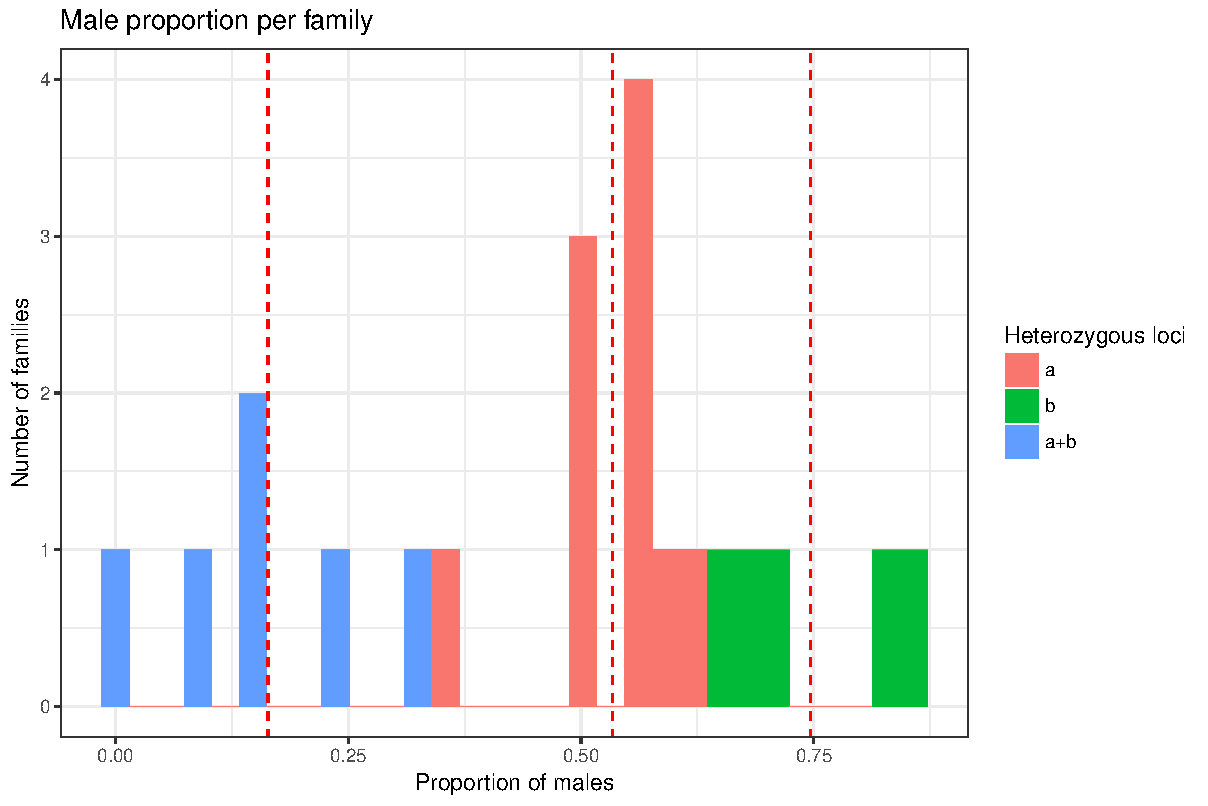
\includegraphics[width=1\textwidth]{Num_CSD_loci/Group_mother_21fam_3gr.pdf}
		\caption{Distribution of families according to inferred proportion of males among diploid offspring considering 2 CSD loci. Families are separated into 3 groups depending on which loci are expected to be heterozygous in the mother. Families were grouped using 1D k-means clutering and vertial dashed lines represent the center of each cluster.}
		\label{cat_2L_21F}
	\end{center}
\end{figure}

\begin{figure}[h]
	\begin{center}
		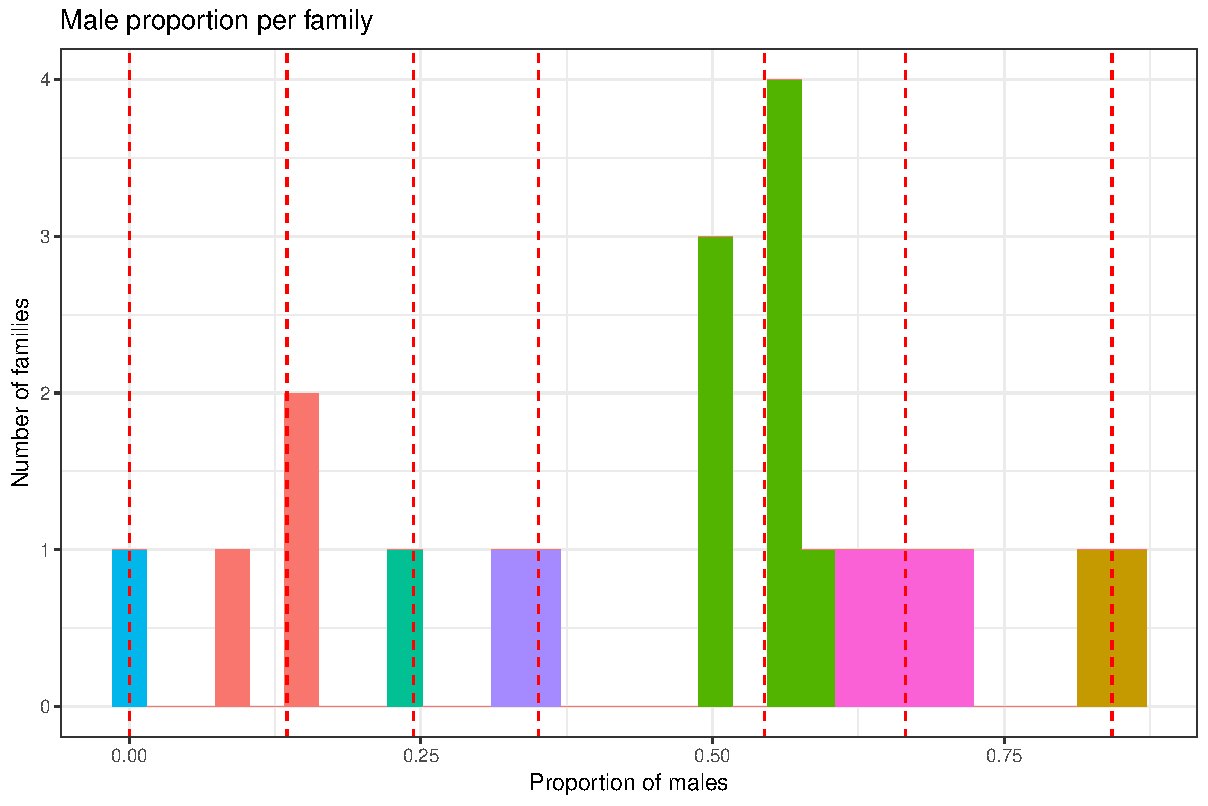
\includegraphics[width=1\textwidth]{Num_CSD_loci/Group_mother_21fam_7gr.pdf}
		\caption{Distribution of families according to inferred proportion of males among diploid offspring considering 3 CSD loci. Families are separated into 7 groups depending on which loci are expected to be heterozygous in the mother. Families were grouped using 1D k-means clutering and vertial dashed lines represent the center of each cluster.}
		\label{cat_3L_21F}
	\end{center}
\end{figure}

\FloatBarrier
\section{Distance to centromeres}

To validate hits, I will use the information of the distance from centromere. The position of the centromere in the scaffold (i.e. metacentric vs telocentric chromosome) can be inferred from the recombination rates along the chromosome. The method I am going to use for this is to measure the proportion of offspring homozygous at each SNP that is heterozygous in the mother (i.e. proportion of recombinant offspring at that SNP).The centromere should be the region with the lowest value.
The hits obtained for CSD candidates in the different categories should be coherent with this distance; the hit in the family with a low diploid male production should be closer to the centromere.\\

Modelling the recombination rate along chromosomes using a weighted loess (lowess) curve revealed local minima that could contain centromeres, however the position of these minima can vary strongly depending on the span (smoothing parameter) allowed for local regression when building the curve. This is likely due to the small number of individuals, or rarity of recombination events. The proportion of homozygosity also tends to decrease far from centromere, this is likely due to multiple recombination events restoring heterozygosity. Note the curve uses the proportion of recombinant offspring within a family at a given SNP weighted by the total number of offspring in that family.

I tried locating the centromere both by running populations with all individuals pooled together (Figure \ref{centro_all}) and separately for each family (Figure \ref{centro_fam}). If I want to use the minimum estimate of local regressions objectively to locate the centromere, I will need to use some form of cross validation to estimate the span. I could also use a visually optimal value for span; the default value used in ggplot's geom\_smooth() is 0.75 and seems reasonable on my data (does not seem too noisy).\\


\begin{figure}[h]
	\begin{center}
		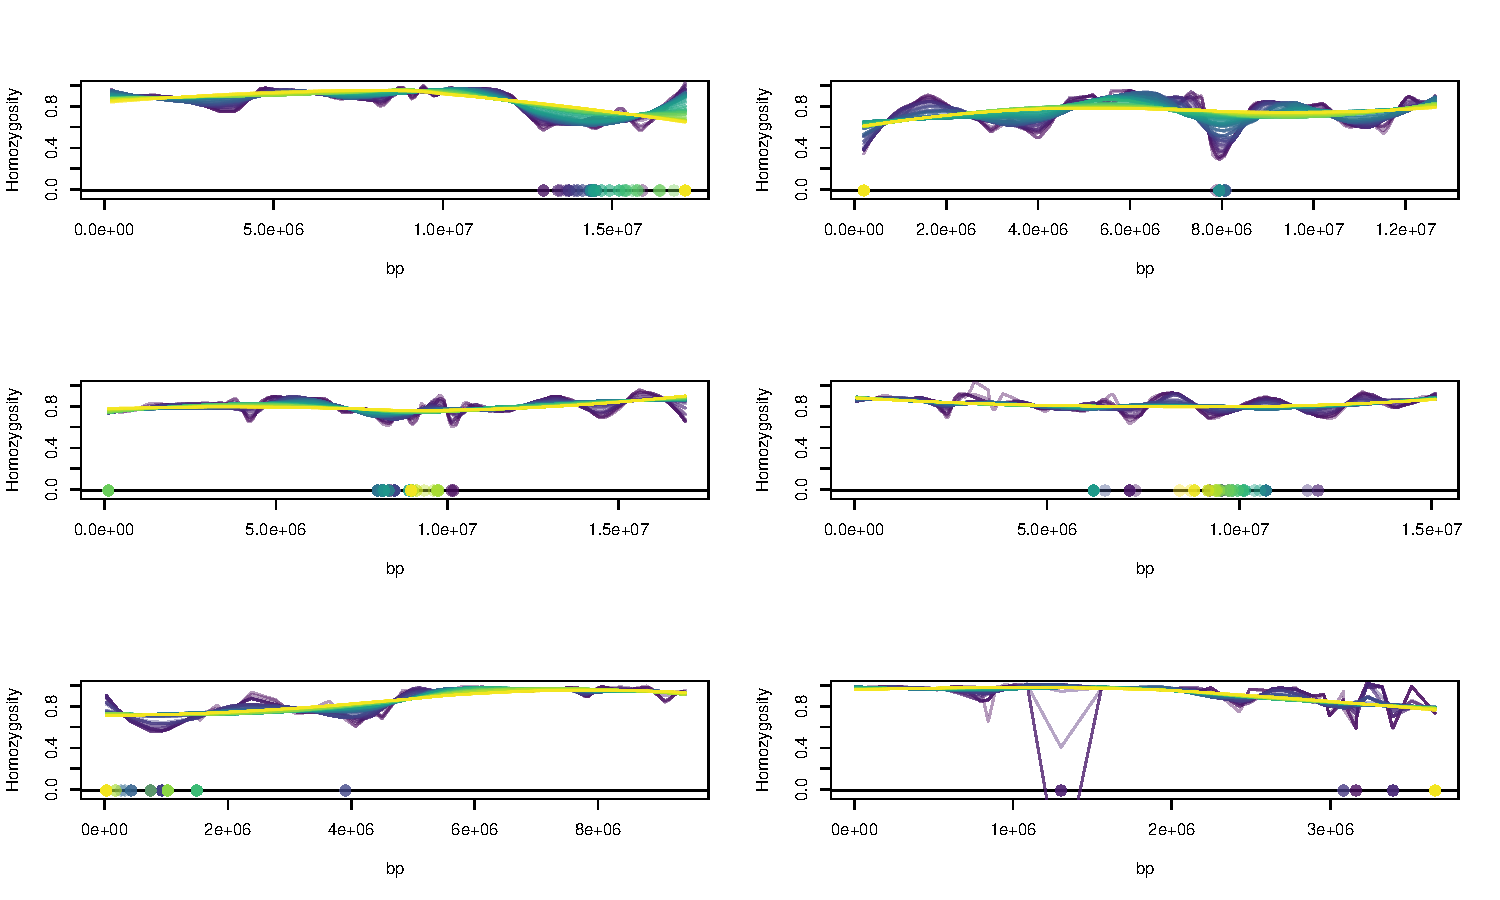
\includegraphics[width=1\textwidth]{Num_CSD_loci/centro_group_d3r80_degree2.pdf}
		\caption{Modelling recombination rates along chromosomes using local regression with second degree polynomials on proportion of homozygous individuals as a proxy. Populations was run on all individuals pooled together (r80, mindepth:3). Colors represent different span value for the local regression and colored dots are the inferred centromere position (i.e. the minumum of the curve) with the corresponding span value.}
		\label{centro_all}
	\end{center}
\end{figure}

\begin{figure}[h]
	\begin{center}
		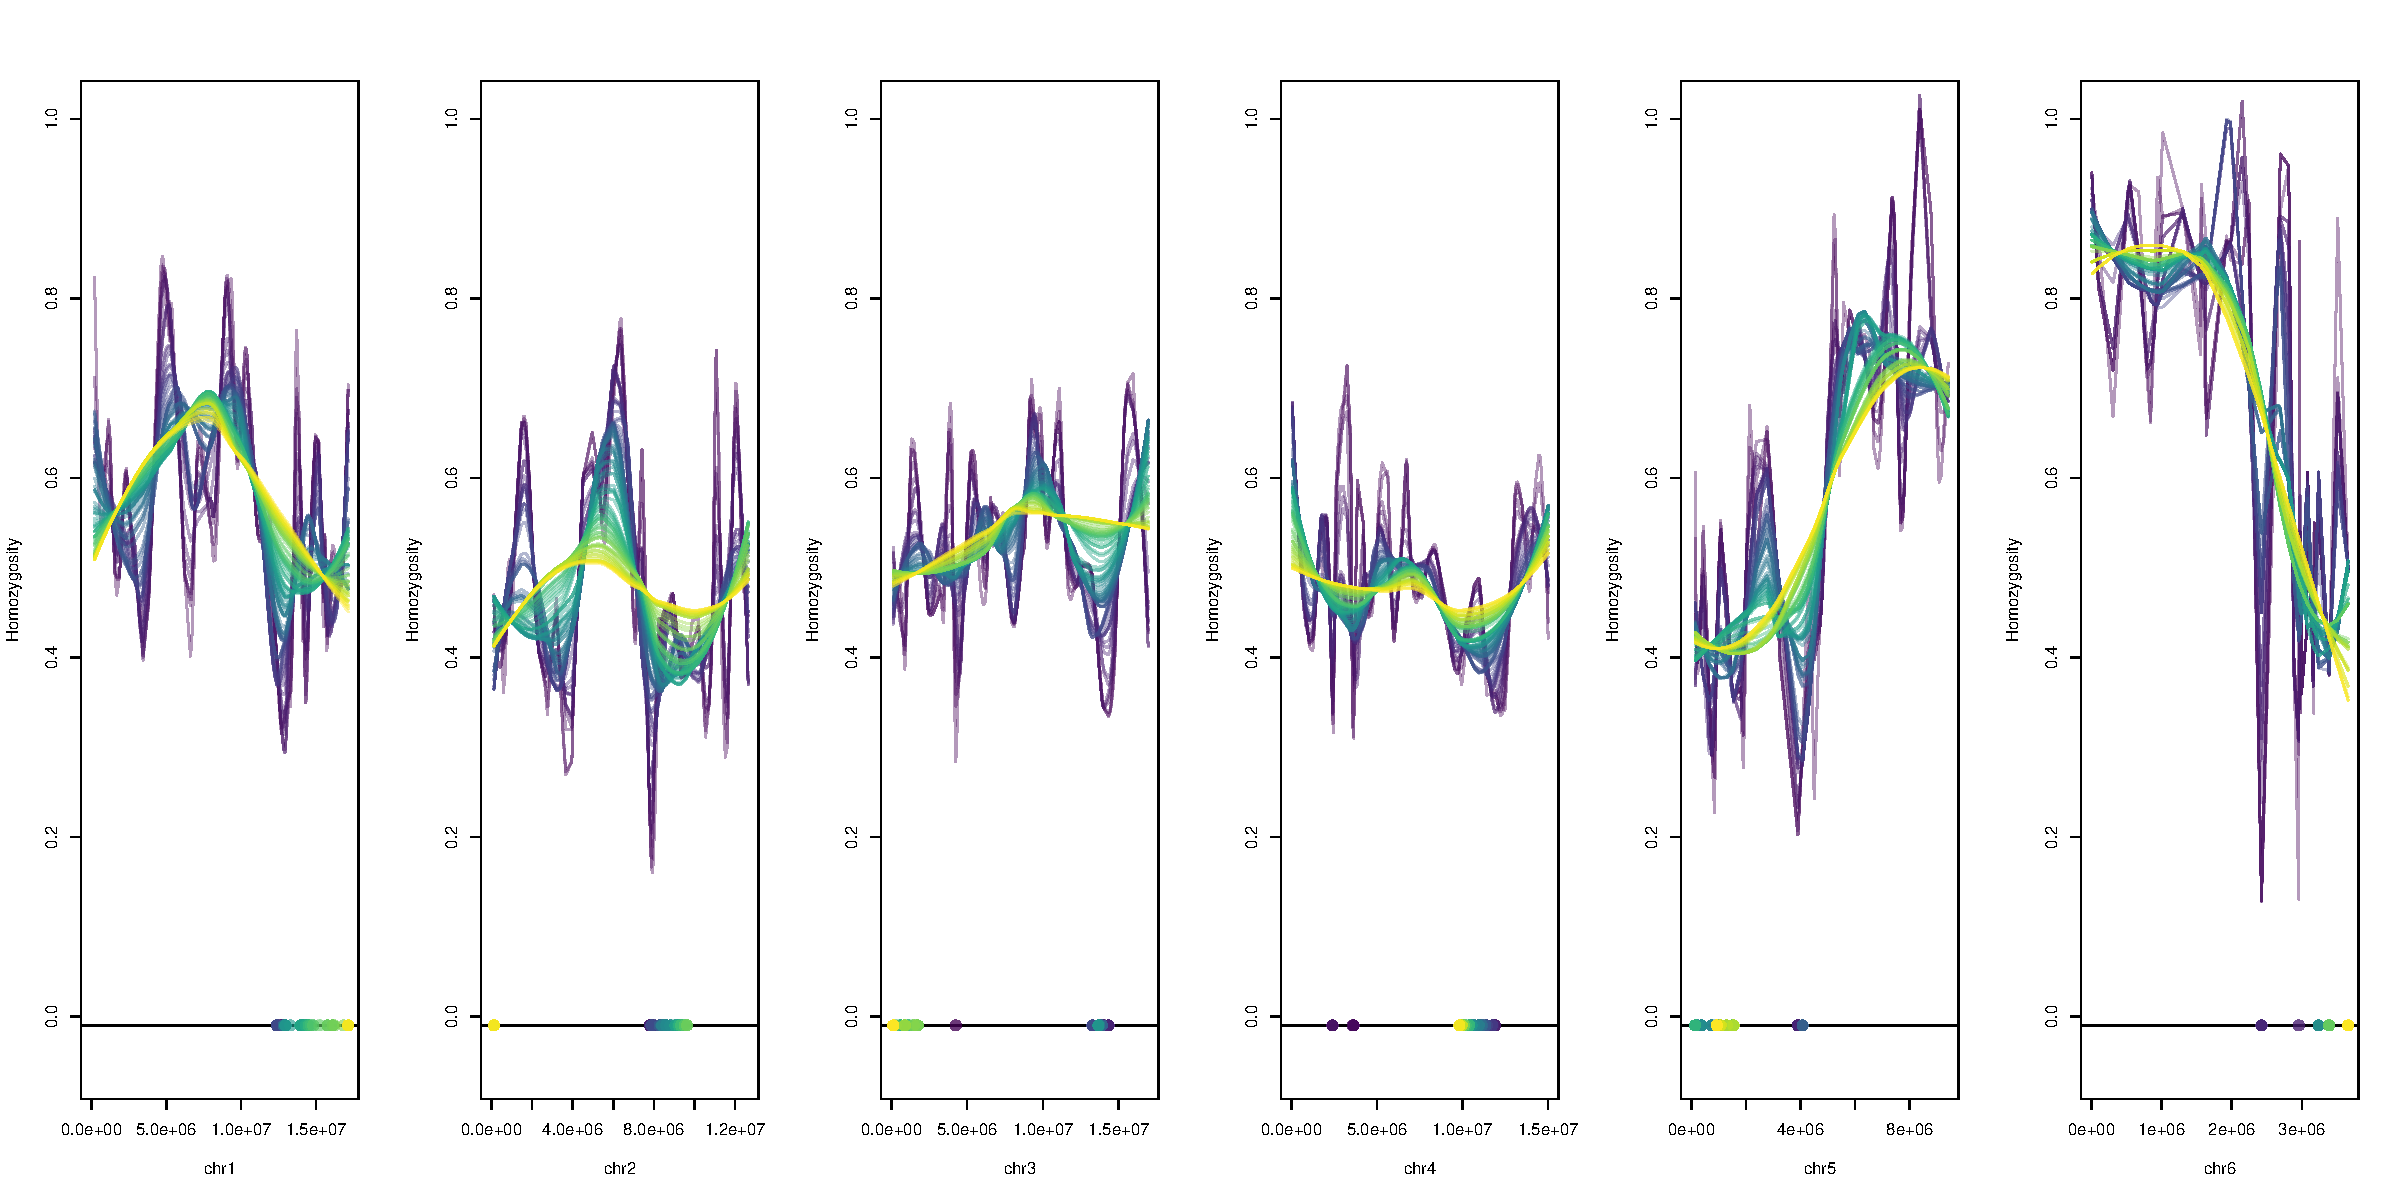
\includegraphics[width=\textwidth]{Num_CSD_loci/centro_fam_d3r80_degree2.pdf}
		\caption{Modelling recombination rates along chromosomes using local regression with second degree polynomials on proportion of homozygous individuals as a proxy. Populations was run on separately for each family, SNPs where the mother is homozygous were removed in each family (r80, mindepth: 3).Colors represent different span value for the local regression and colored dots are the inferred centromere position with the corresponding span value.Colors represent different span value for the local regression and colored dots are the inferred centromeres position (i.e. the minumum of the curve) with the corresponding span value.}
		\label{centro_fam}
	\end{center}
\end{figure}


Date: 12.08.2017

To obtain better result when trying to locate centromeres, I used the genomic output from populations to include fixed SNPs. I subsequently removed all SNPs that are \textbf{either missing or homozygous} in the mother from its whole family (including itself). The variation induced by the span parameter when using local regression is now much smaller. To make sure the centromeres are called correctly, I tried a second simpler method, which consists in computing means over a sliding window on each chromosome. I tried both methods with several different parameter values (Figure \ref{centro_fix}). The methods yielded similar results and I visually selected reasonable parameter values for span and window size to compare the centromeres positions inferred by both methods (Figure \ref{comp_centro}). Centromeres are merely regions and have no objective precise genomic position, besides I will only be interested in relative differences in distance from centromeres to select loci, therefore the parameter values I chose will probably have little to no effect on the results. 

\begin{figure}[h]
	\begin{center}
		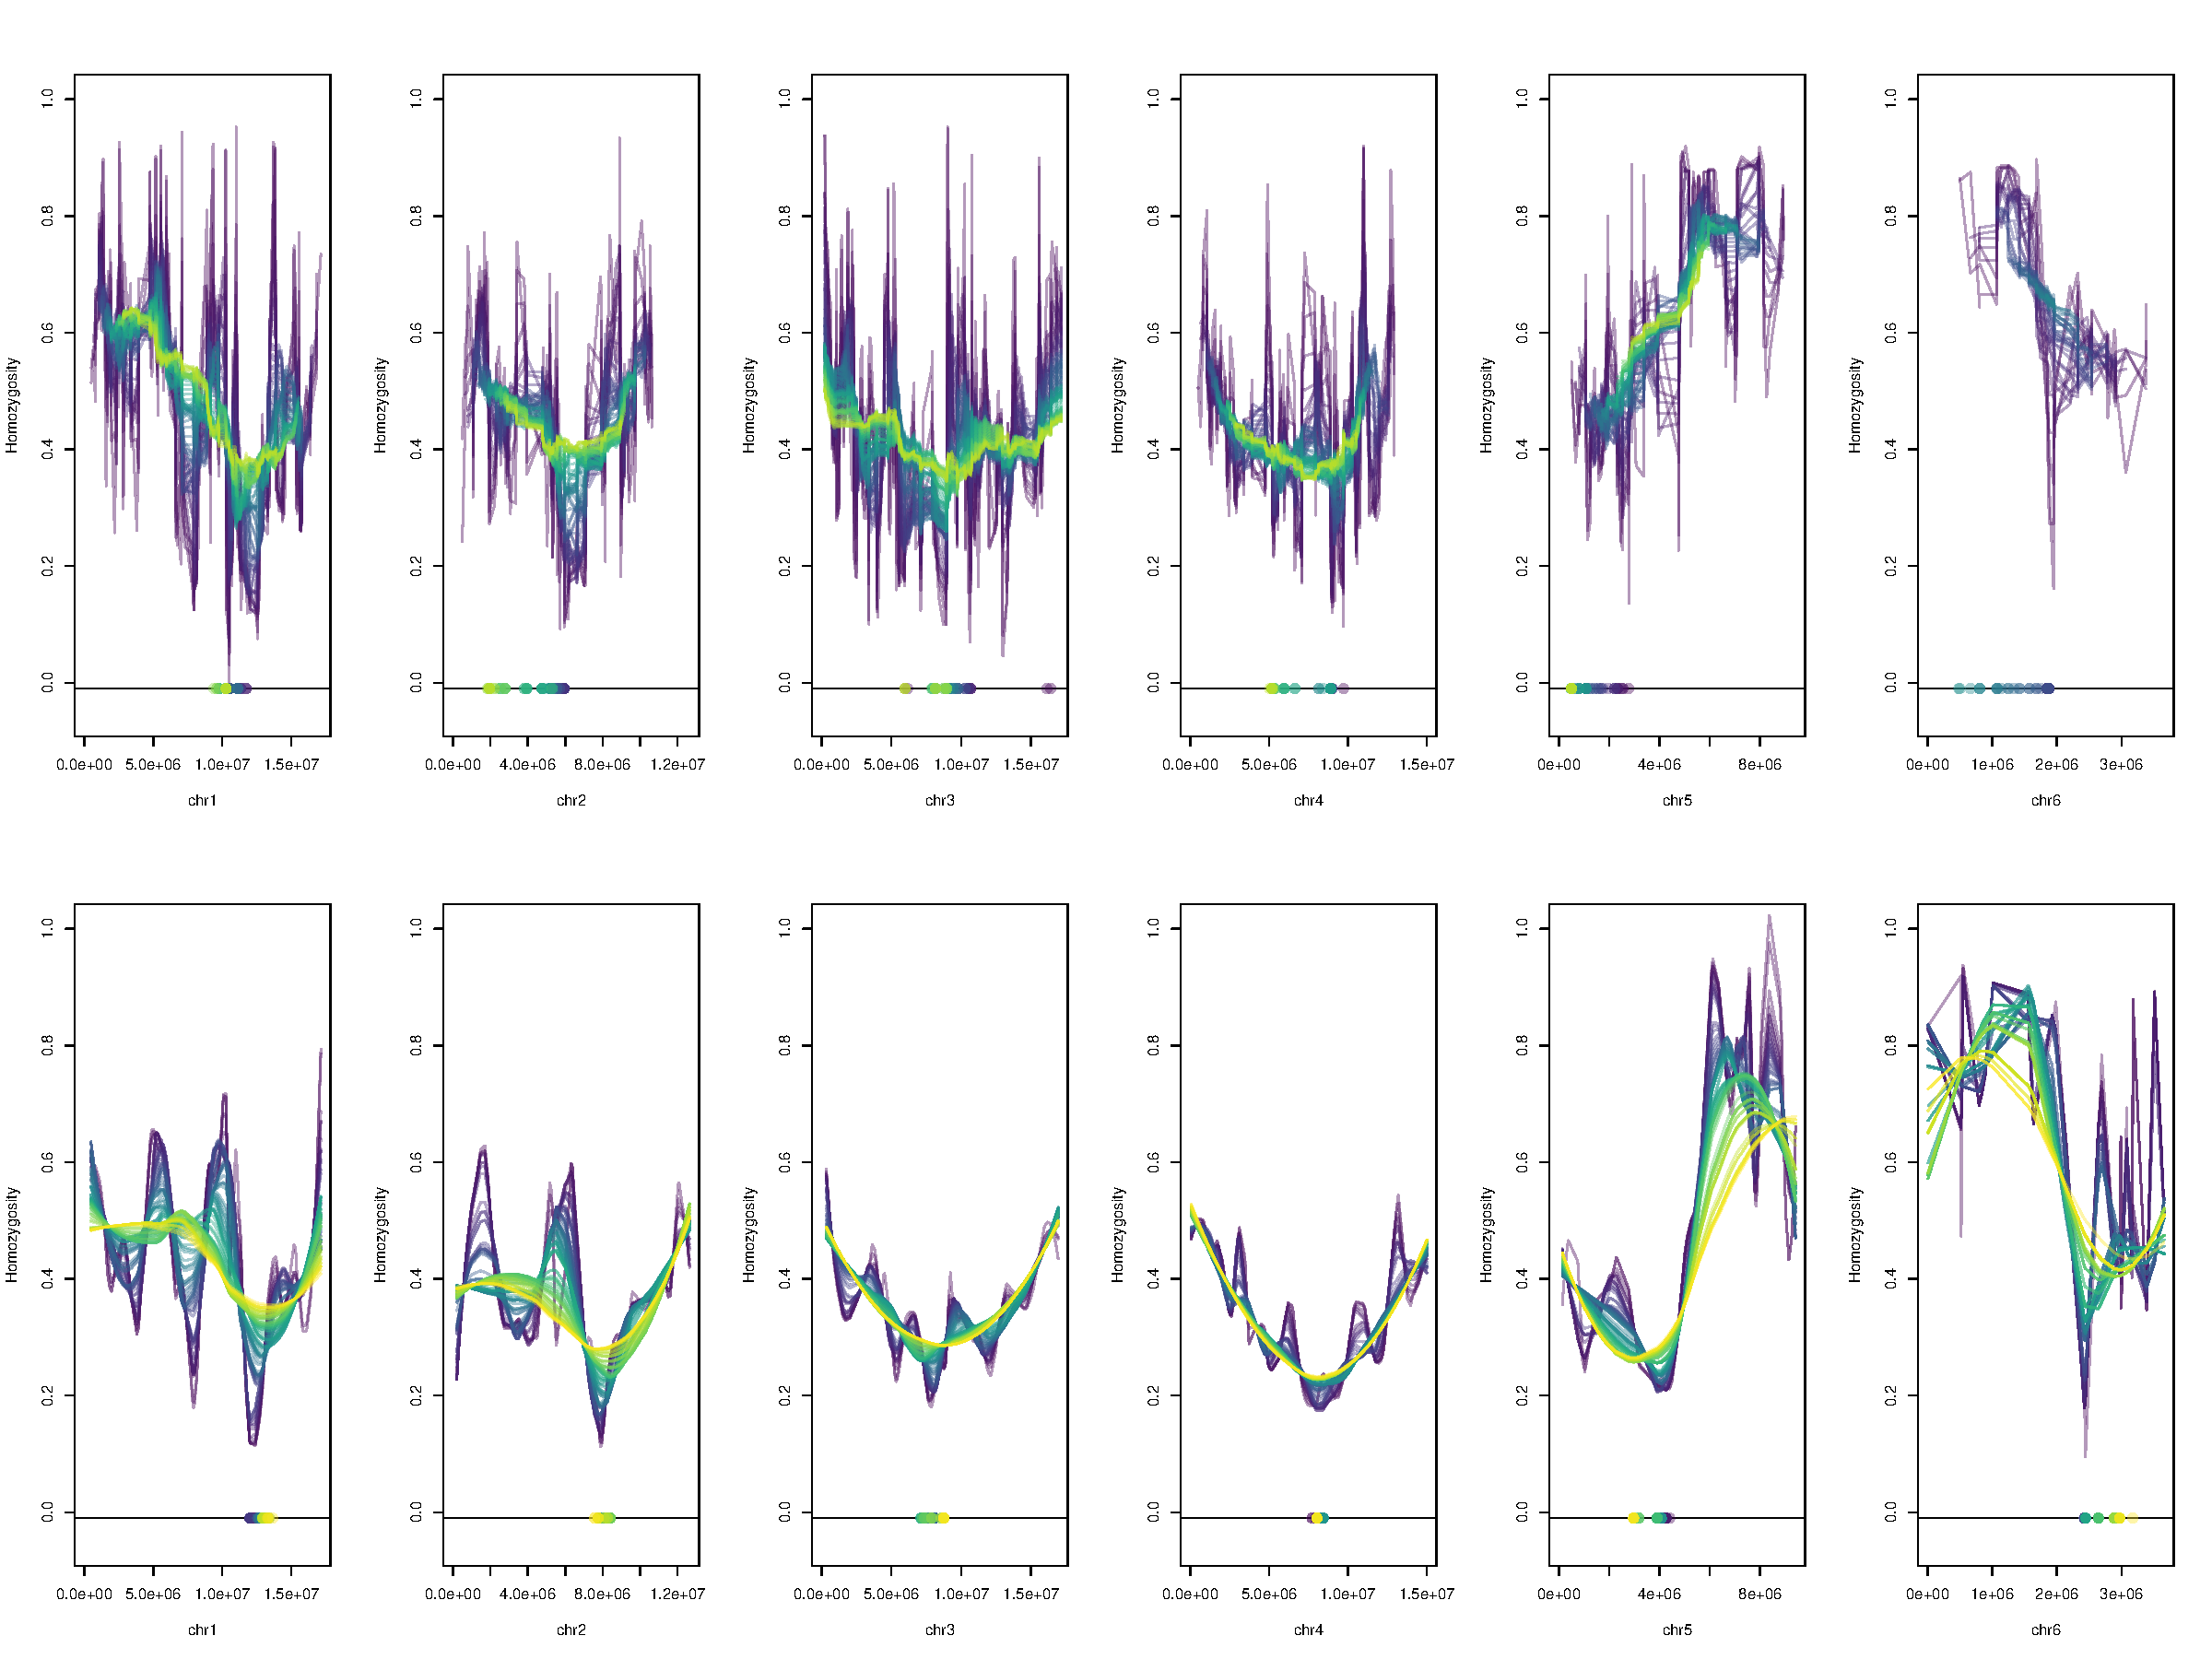
\includegraphics[width=\textwidth]{Num_CSD_loci/centro_group_fix_d3r80_range.pdf}
		\caption{Comparing moving averages and local regression with second degree polynomials to approximate recombination rates. Populations was run on all individuals pooled together. Fixed SNPs are included and SNPs where the mother is homozygous or that were absent in the mother were removed in each family (r80, mindepth: 3). Range of parameter tested: span varied between 15\% and 100\% of observations by intervals of 1\% for local regression and window size between 3 and 80 observations with intevals of 1 for moving averages. Colors represent the different span or window size value for the local regression and colored dots are the inferred centromeres position (i.e. the minimum of the curve) with the corresponding parameter value.}
		\label{centro_fix}
	\end{center}
\end{figure}

\begin{figure}[h]
	\begin{center}
		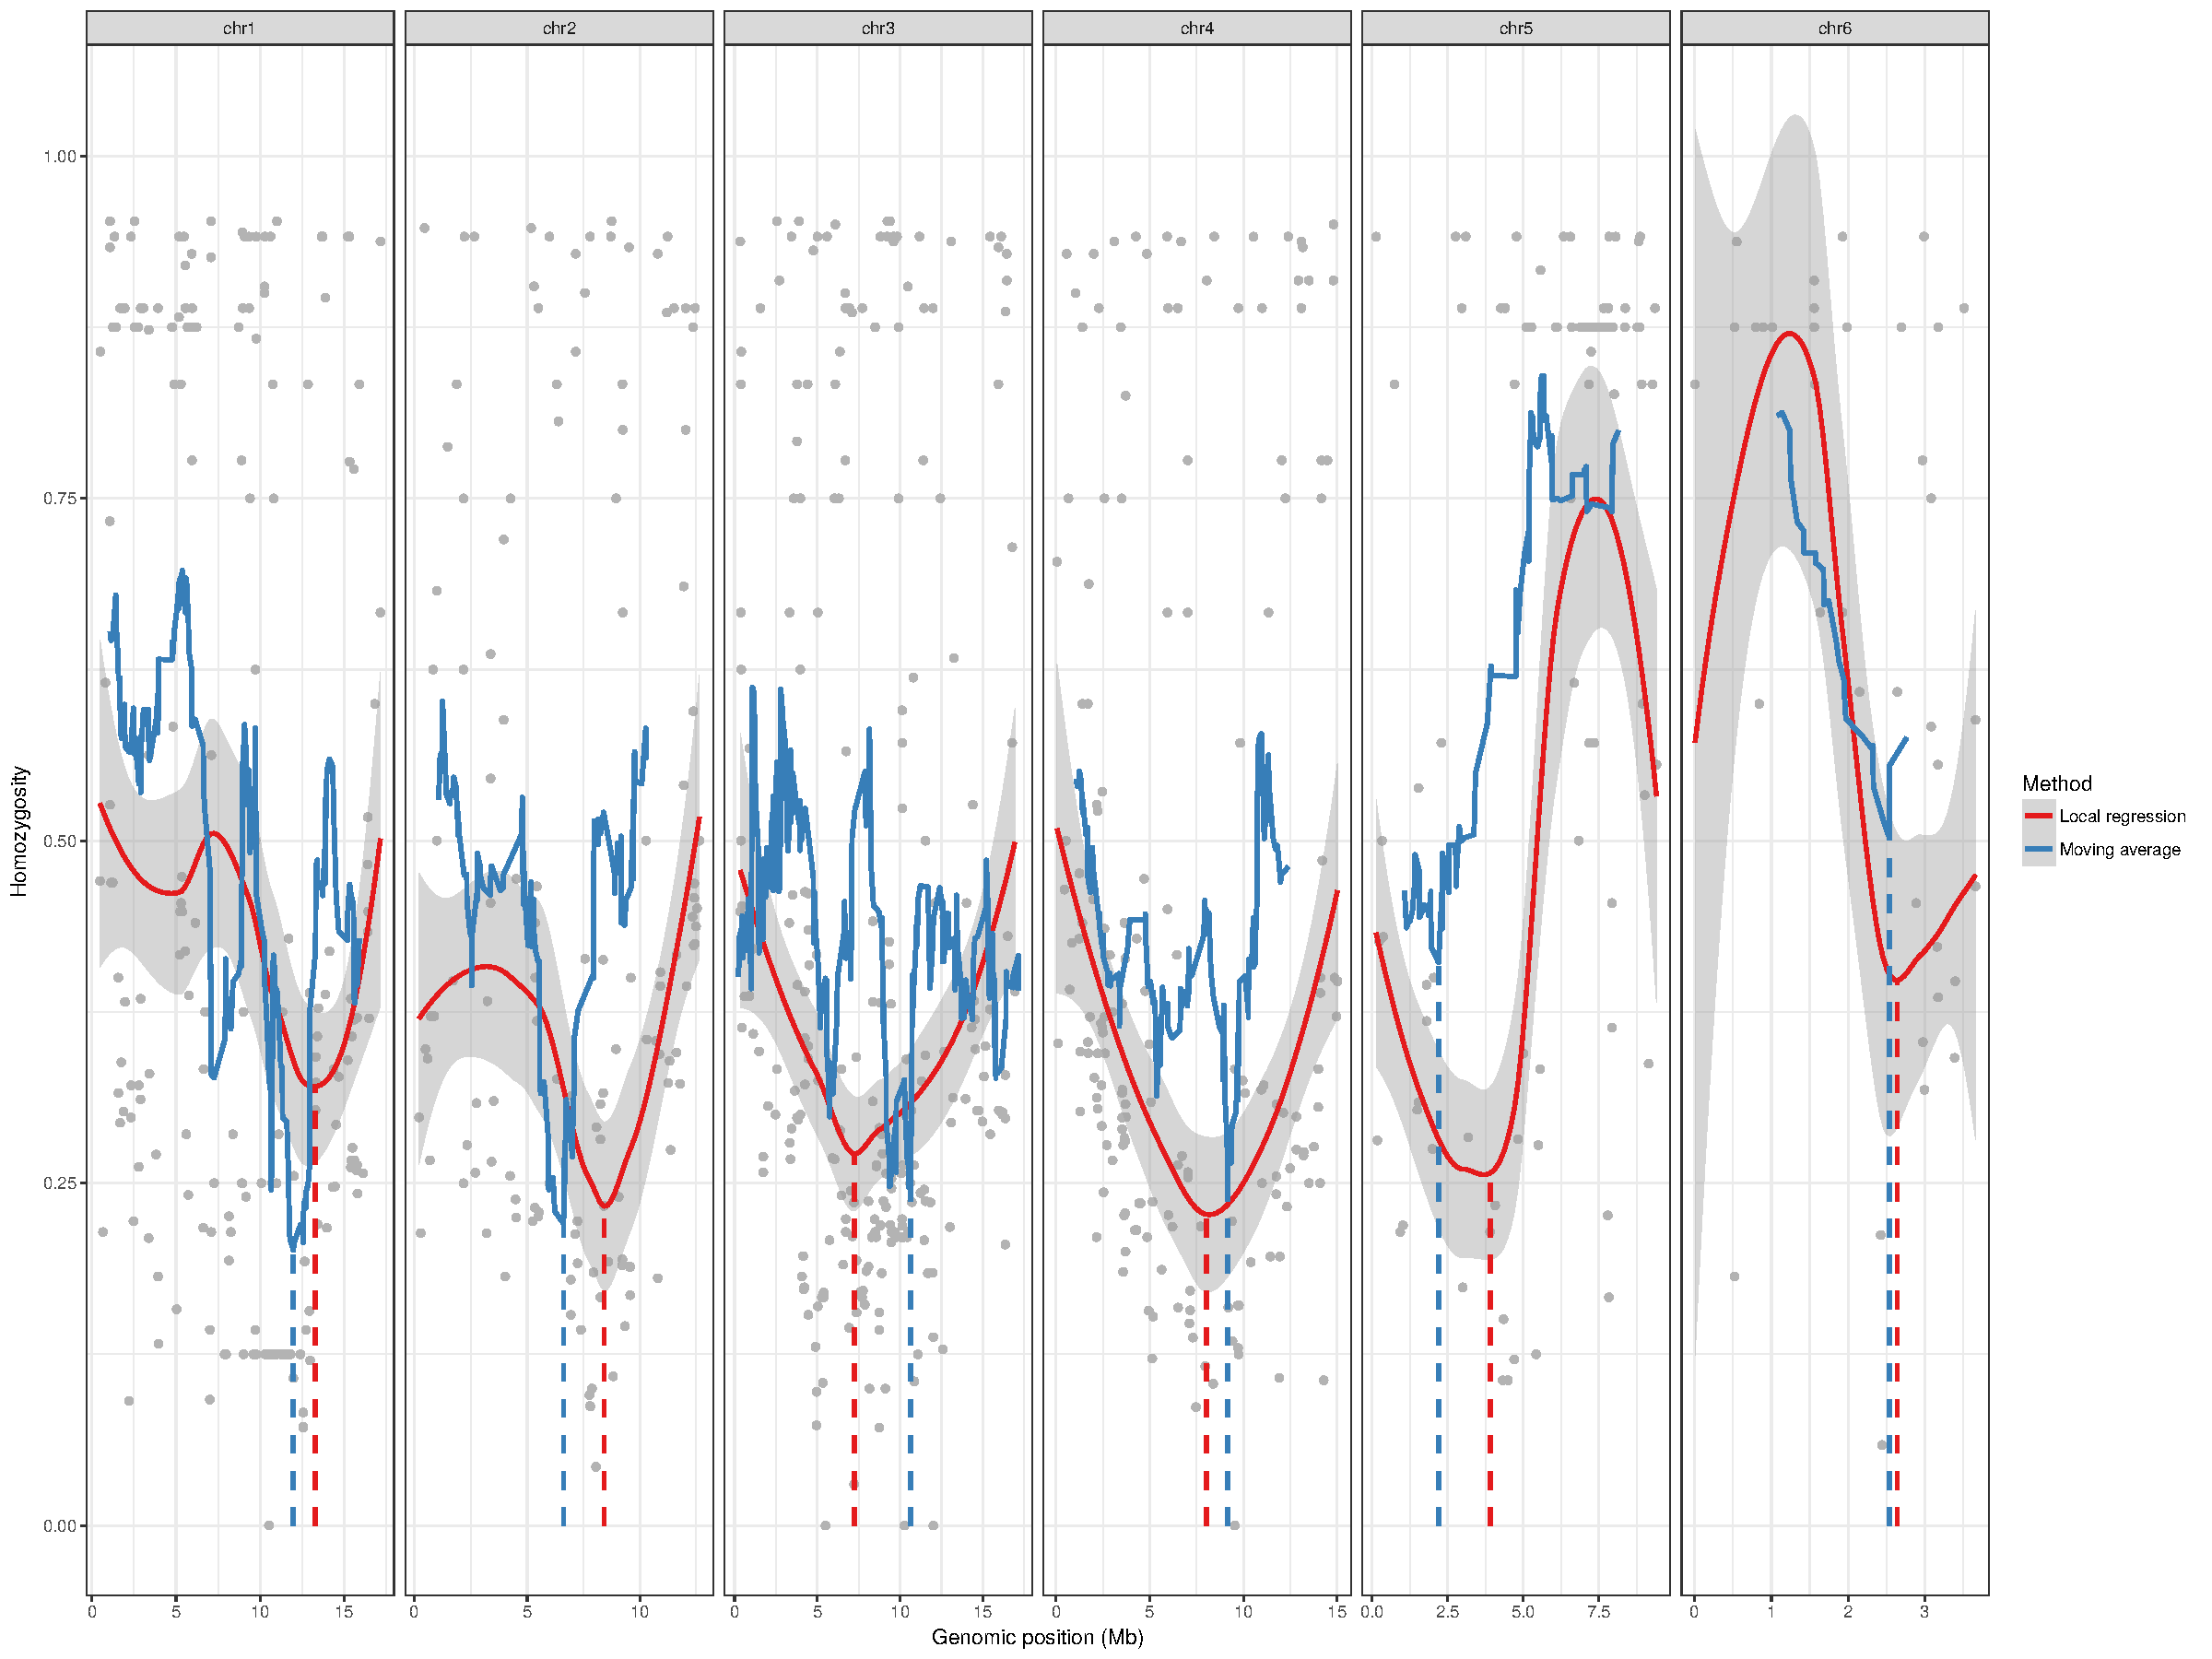
\includegraphics[width=1.1\textwidth]{Num_CSD_loci/centro_group_fix_d3r80_final.pdf}
		\caption{Comparing moving averages and local regression with second degree polynomials to approximate recombination rates. Populations was run on all individuals pooled together. Fixed SNPs are included and SNPs where the mother is homozygous or that were absent in the mother were removed in each family (r80, mindepth: 3). Parameters selected for comparison: window size: 20, span: 0.75. Dotted lines show the inferred centromeres position (i.e. the minimum of the curve) with both methods.}
		\label{centro_fix}
	\end{center}
\end{figure}

\FloatBarrier

\subsection{Terminal or central fusion}

Date: 31.08.2017\\

When modeling heterozygosity along the genome, there were interferences (waves) and the putative centromeric regions are not fully heterozygous. This could be due to several factors (inclusion of 
haploids, sequencing errors, errors in linkage map...). One of the more likely reasons, could be that 
some individuals are produced by terminal fusion automixis, rather than central fusion, which would cause
them to be homozygous at the centromere and affect the whole model.\\

A way to test this, which has already been used in Daphnia (Svendsen et al, 2015), is to model the heterozygosity relative to the mother of each offspring as a function of the distance from the centromere. All chromosomes are pulled together. Note the Svendsen uses centimorgans and I use physical distance in basepair.

I visualise it in two ways:\\
First, using a sliding window moving away from the centromere in absolute distance (Figure \ref{proto_slide_fusion}). Each sliding window computes the proportion of heterozygous sites in each individual. \\
Second, choosing different sizes for the putative centromeric region and computing the proportion of heterozygous with each value (Figure \ref{proto_surround_fusion}). Under central fusion, one would expect the heterozyosity to decrease when the window moves away from the centromere, or when the putative region is enlarged. On the other hand, under terminal fusion, the value should increase when moving away or increasing the size of the centromeric region.

\begin{figure}[h]
	\begin{center}
		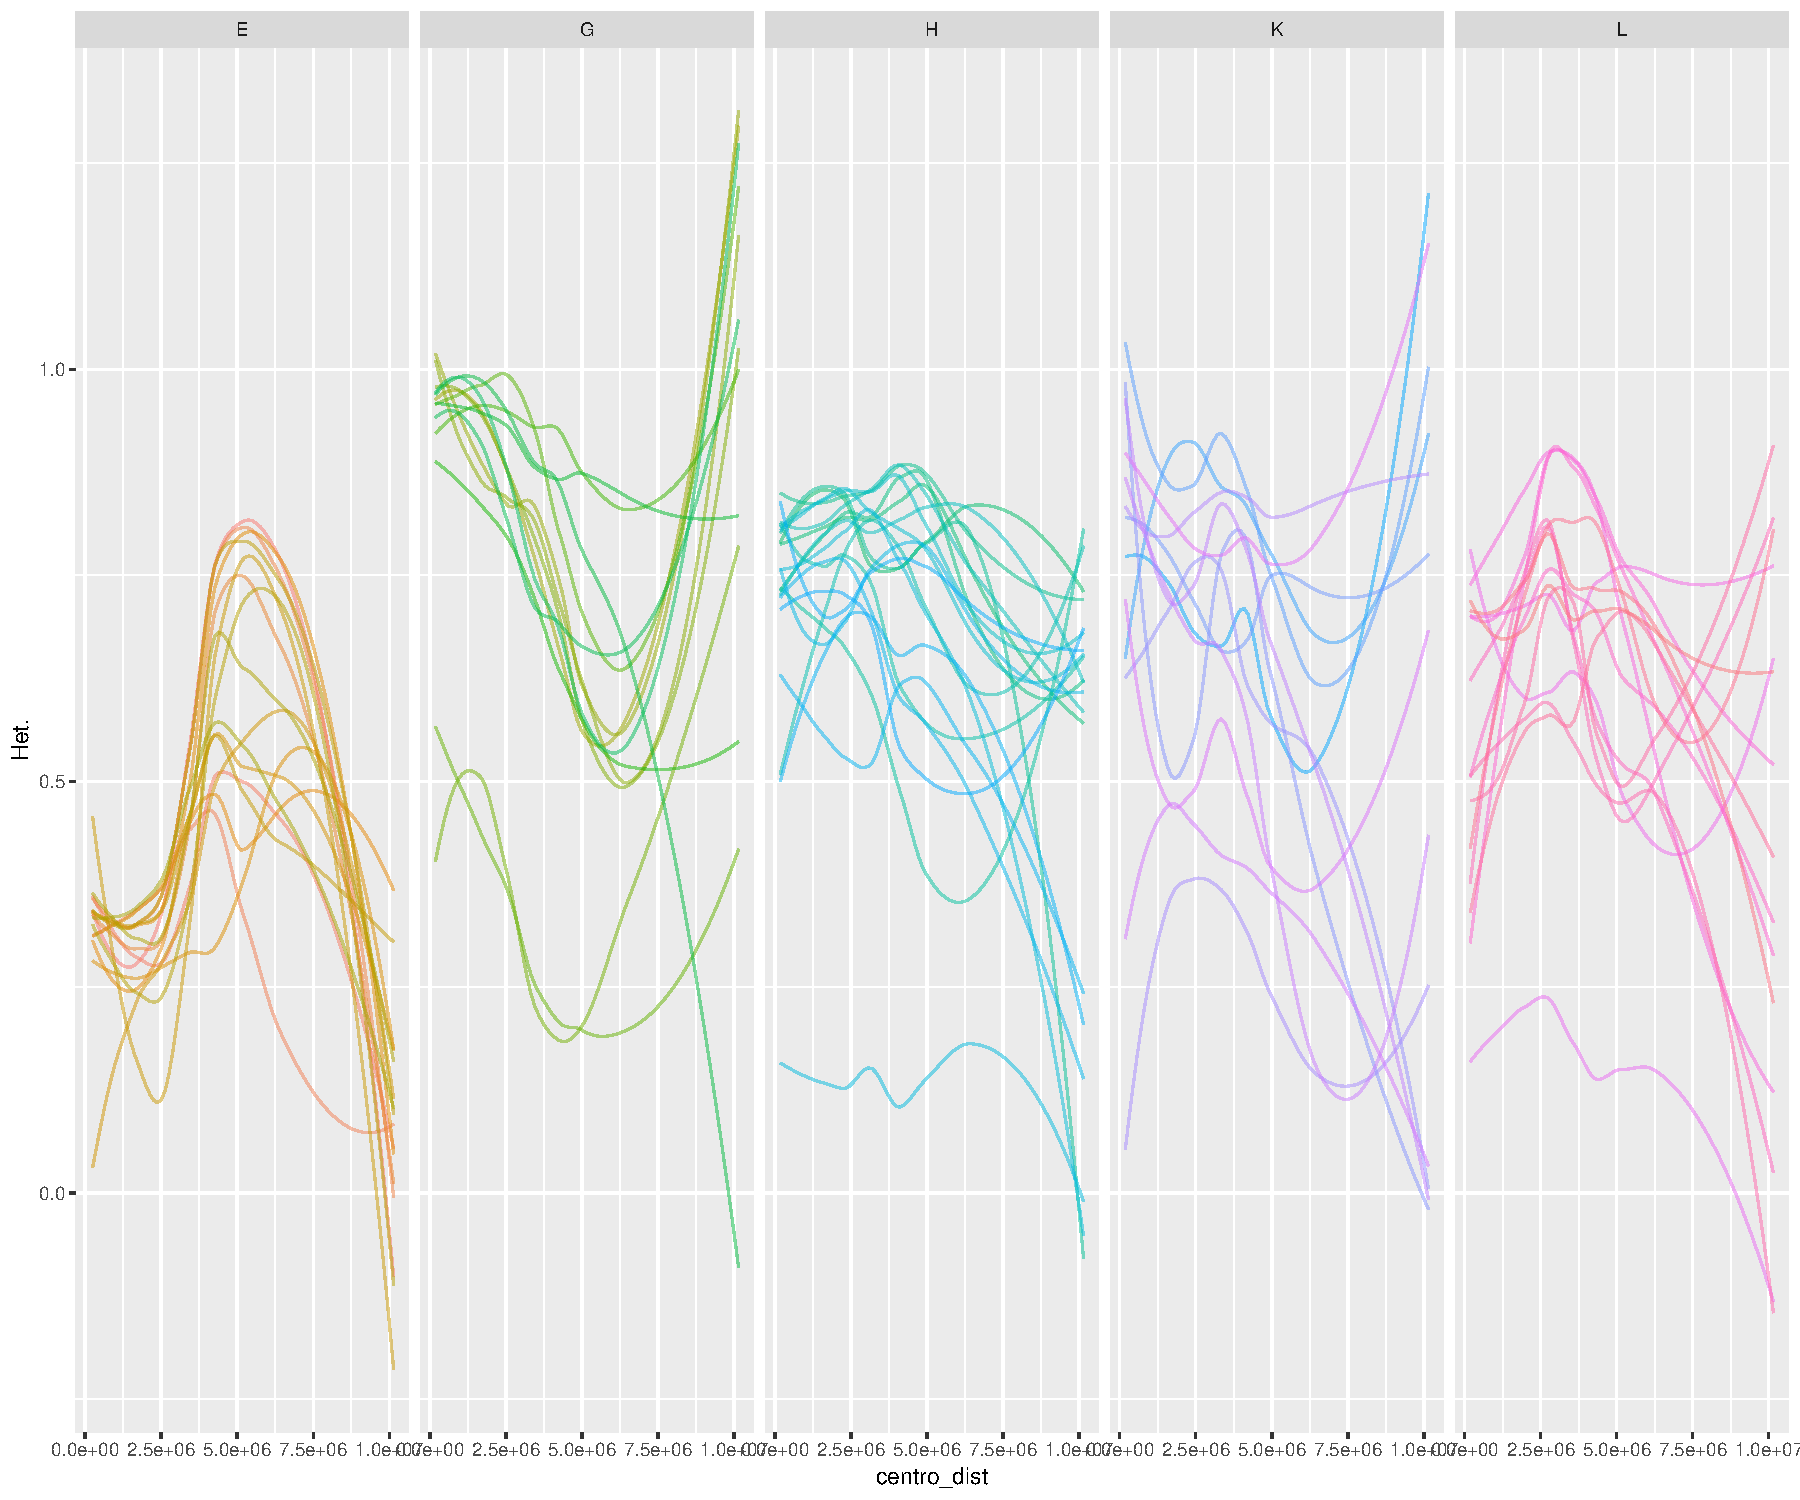
\includegraphics[width=1.1\textwidth]{Num_CSD_loci/pooled_chr_centro_dist_win30.pdf}
		\caption{Modeling the proportion of heterozygosity as a function of the distance from the centromere in each individual separately. Proportions are calculated in sliding windows, each containing 30 SNPs and the base pair at the middle of the window is used for plotting. The curves are obtained by local regression (loess). All chromosomes are pulled together in a single figure}
		\label{proto_slide_fusion}
	\end{center}
\end{figure}

\begin{figure}[h]
	\begin{center}
		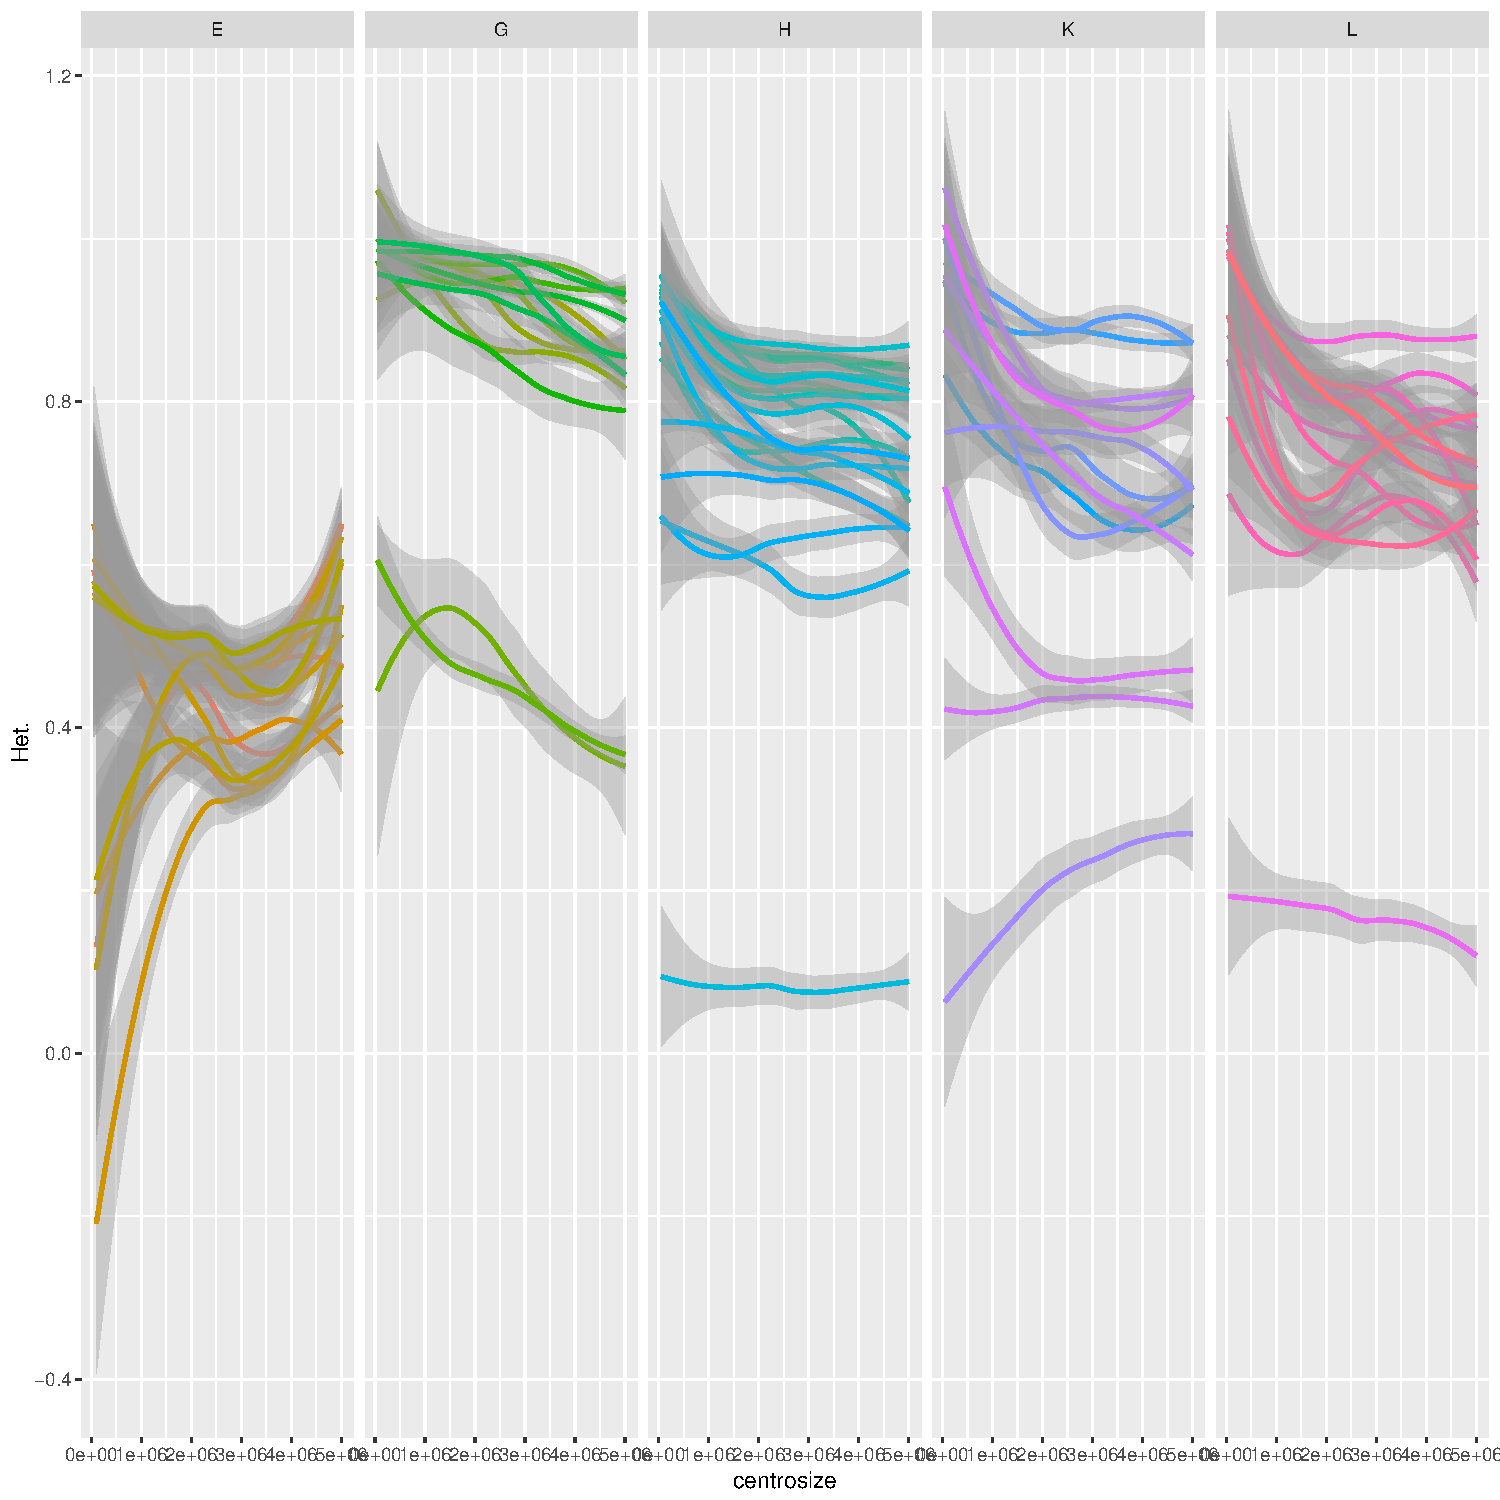
\includegraphics[width=0.8\textwidth]{Num_CSD_loci/pooled_chrom_centrosize_50k_5M.pdf}
		\caption{Measuring the proportion of heterozygous sites relative to mother in regions of variying size between +/- 50kb and +/- 5Mb around centromere in each individual. Panes represent families (only 5 largest ones included) and chromosomes are pooled together. The curves are obtained using a local regression (loess).}
		\label{proto_surround_fusion}
	\end{center}
\end{figure}

Given the density of SNPs in my data, these methods cannot be used to reliably identify central or terminal fusion. There is also the possibility that some scaffolds are inverted in the linkage map, which would strongly affect the results.\\

tl;dr : I don't think I can pull anything useful from this, data is too noisy. \\

\FloatBarrier
Update: 13.09.2017\\
To differentiate more reliably central vs terminal fusion individuals, I used a simpler method (Figure \ref{schema_cen_tel}). After transforming basepair coordinates in each chromosome into absolute distance from centromere, I separate each chromosome into 2 windows: "centro" for centromeric region and "telo" for telomeric region. The centromeric region contains all SNP located closest to the centromere within 25\% of the maximum distance to centromere recorded in the chromosome, while the telomeric region contains those in the furthest 25\%. I compared the proportion of heterozygous SNPs in the two windows, first separating chromosomes (Figure \ref{cen_tel_chr}). Then, I tried pooling all chromosomes together in each individual and I compared the two windows using a linear model, weighting the value of each chromosome by the number of SNPs contained in the window (Figure \ref{cen_tel_lm}).

\begin{figure}[h]
	\begin{center}
		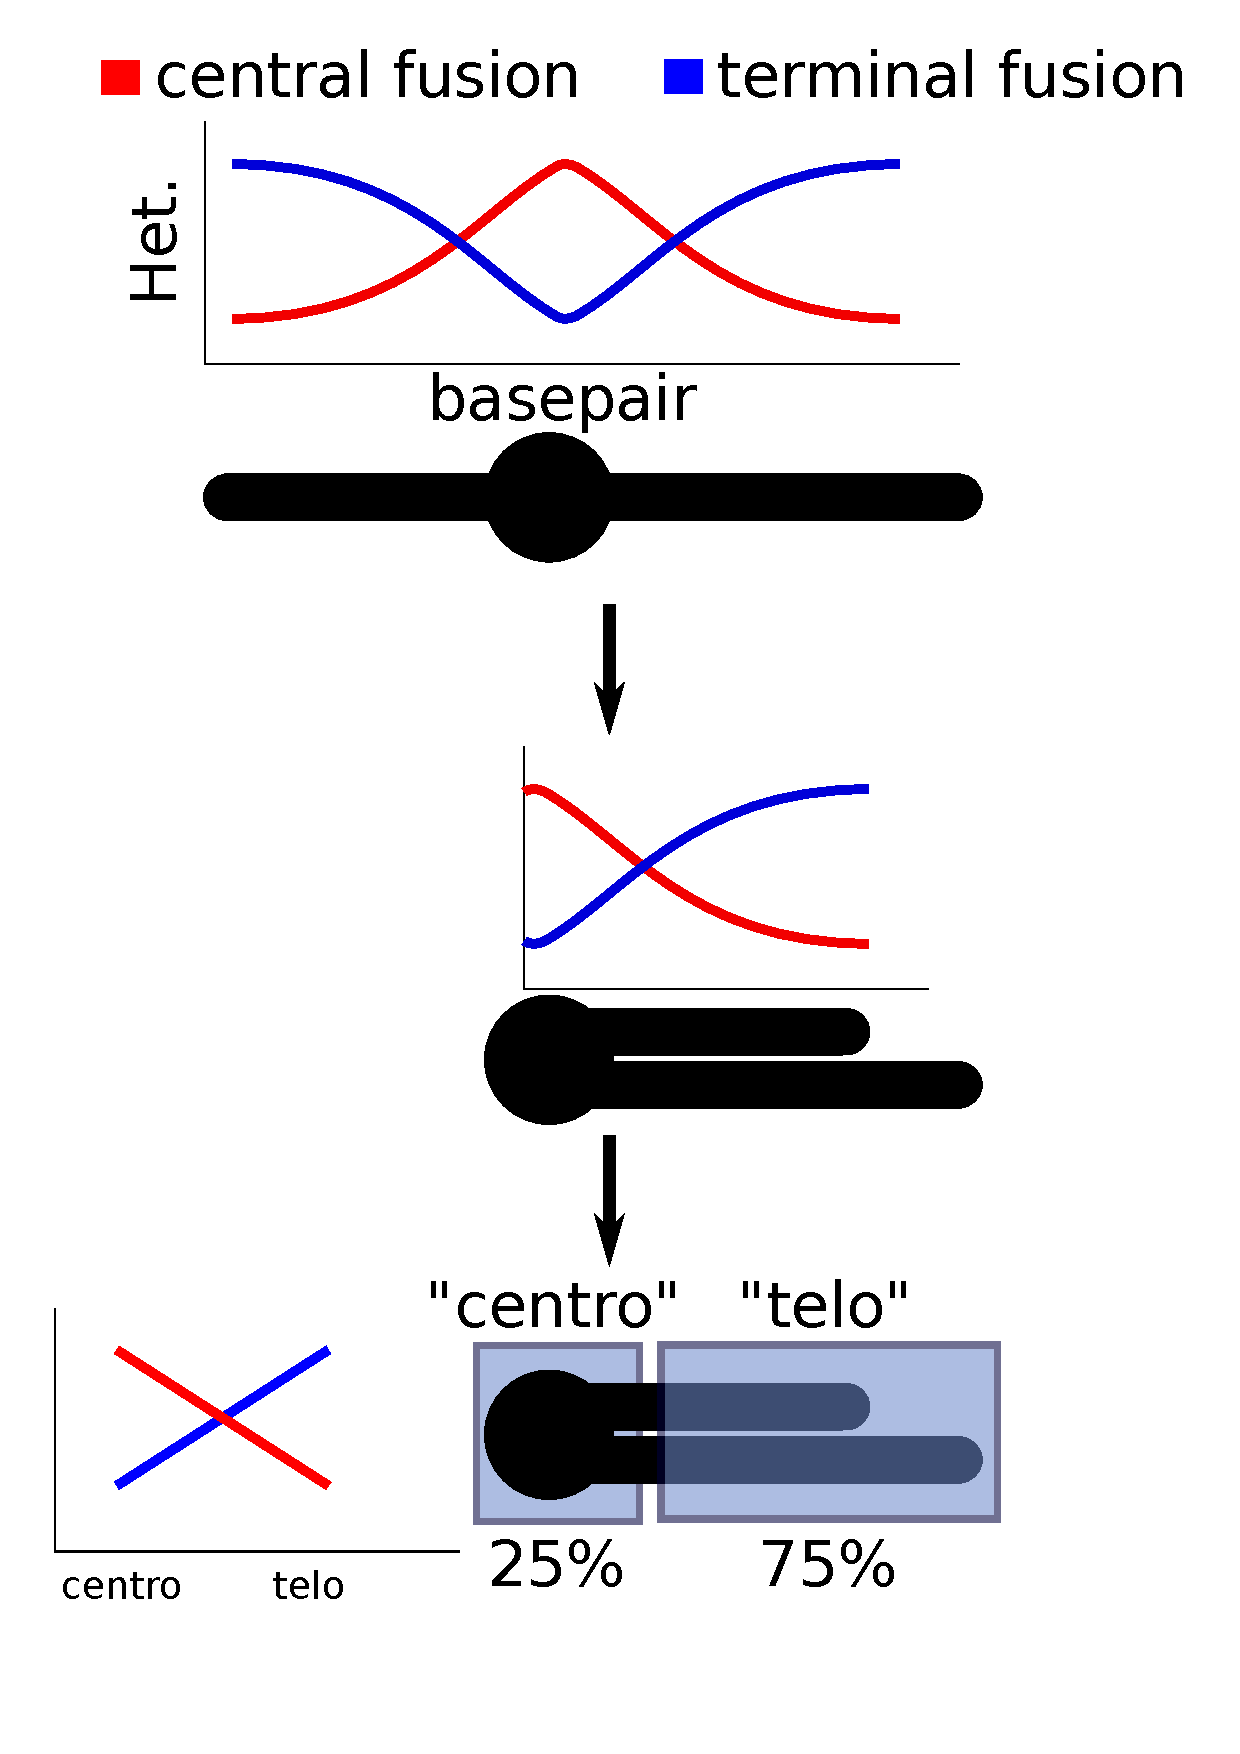
\includegraphics[width=0.5\textwidth]{Num_CSD_loci/cen_tel.pdf}
		\caption{Method used to identify central fusion or terminal fusion individuals from genome-wide heterozygosity. Central fusion individuals (red) are expected to have high heterozygosity values decreasing towards centromeres while terminal fusion (blue) individuals are expected to have low heterozygosity increasing towards centromeres. The basepair coordinates of SNPs are first transformed into absolute distance from centromere. SNPs closer to the centromere than 25\% of the maximum distance to centromere in each chromosome are pooled into one "centromeric" window and those in the 25\% closest to the telomeres are pooled into another "telomeric" window. The proportion of heterozygous SNPs is then computed separately in each window and the difference between those values is used to assign fusion mechanism.}
		\label{schema_cen_tel}
	\end{center}
\end{figure}

\begin{figure}[h]
	\begin{center}
		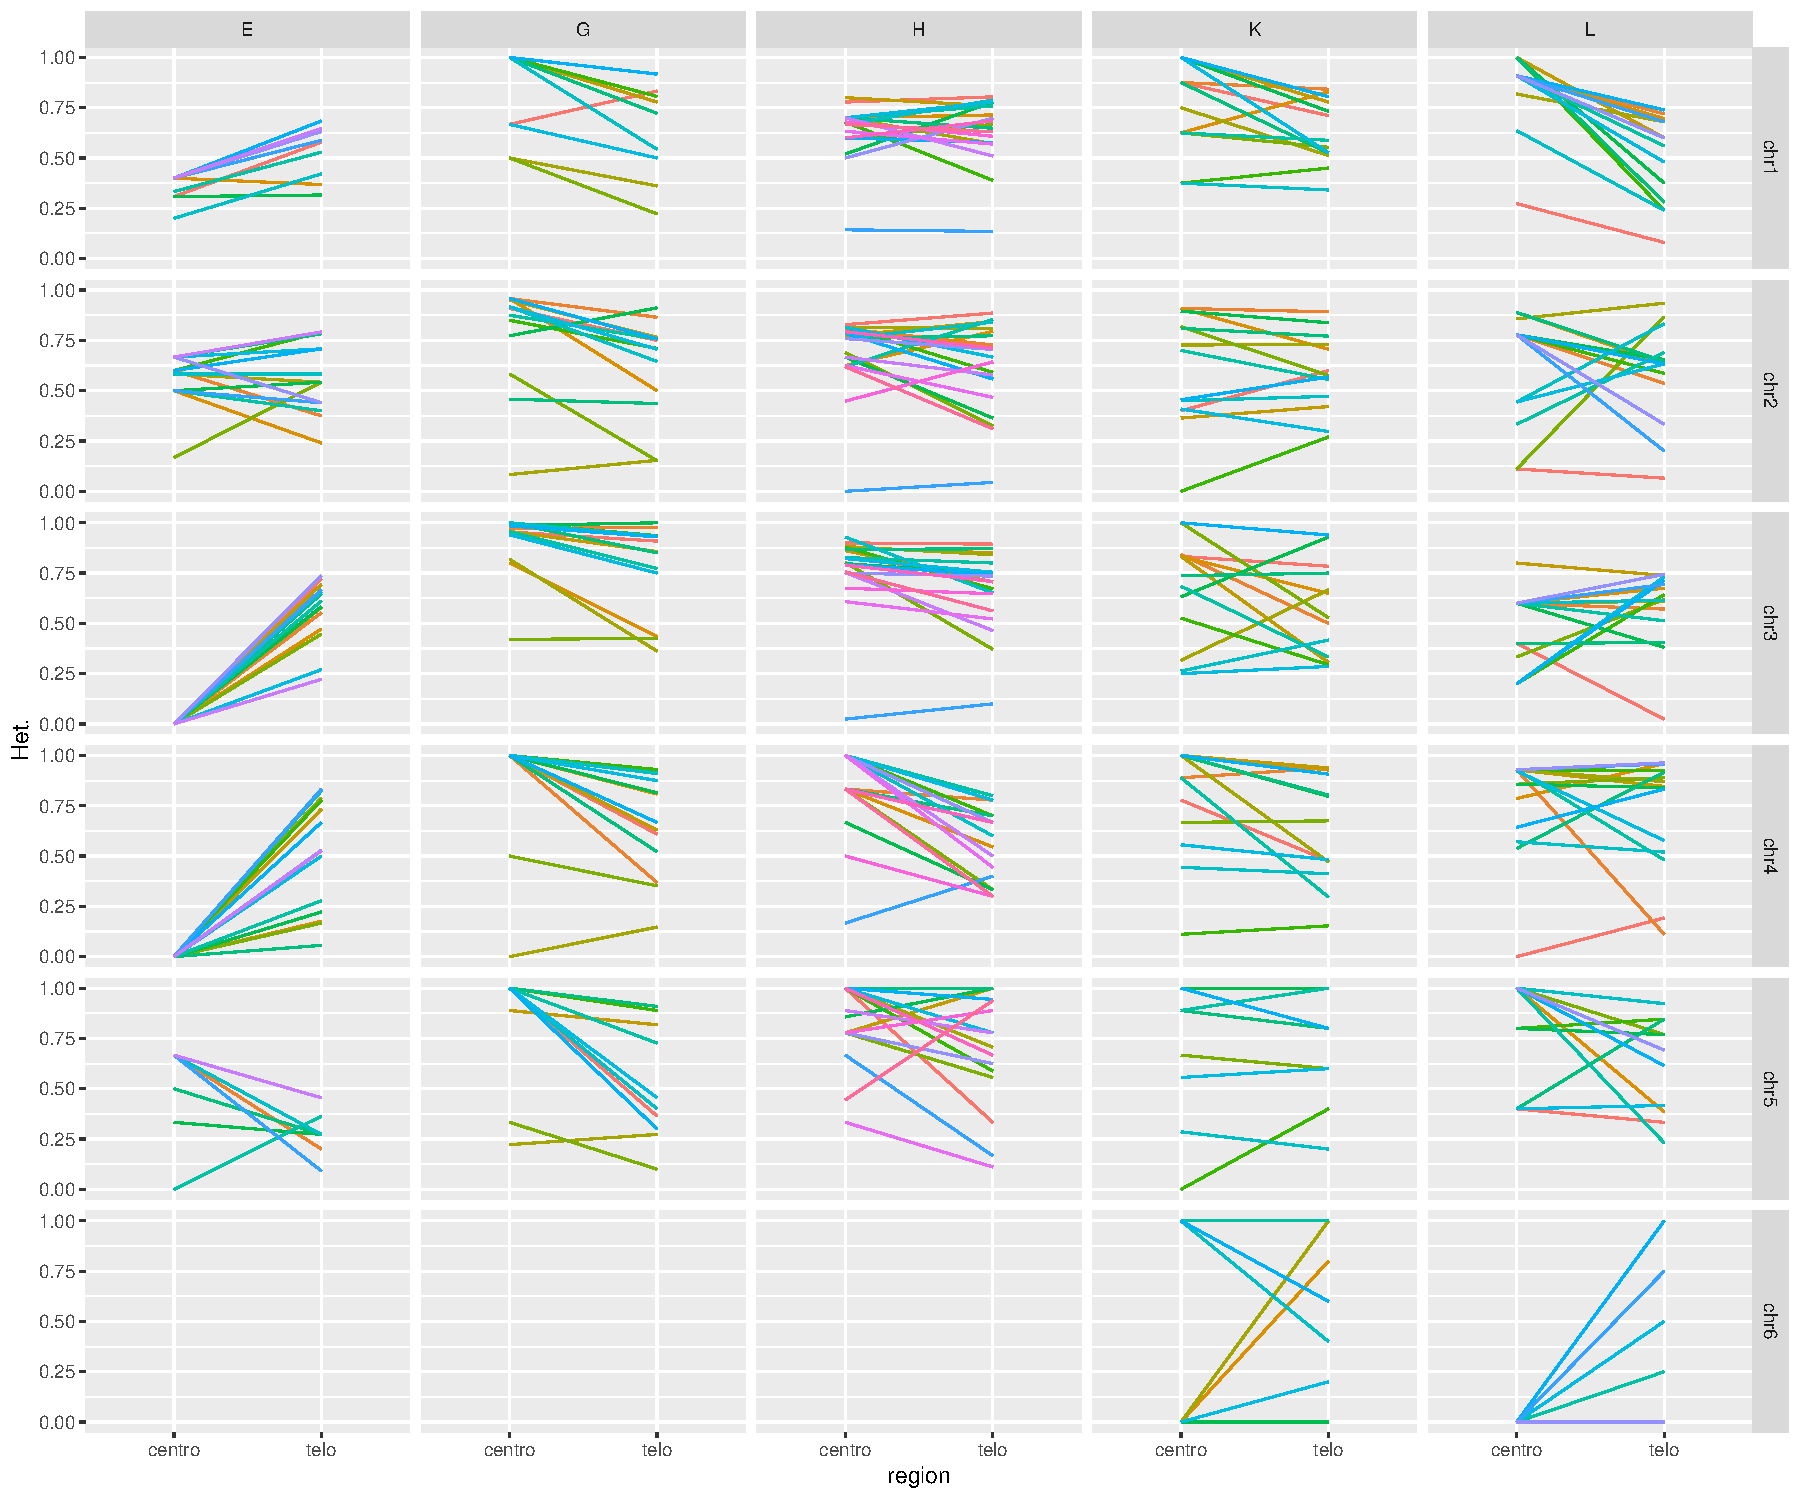
\includegraphics[width=1\textwidth]{Num_CSD_loci/line_centro25_telo_chr_fam.pdf}
		\caption{Comparing the proportion of heterozygous SNPs in each chromosome among variant sites between the centromeric window (SNPs closer than 25\% of maximum distance to centromere) and telomeric window (SNPs further than 75\%). Only the 6 largest families are included for visualisation purpose.}
		\label{cen_tel_chr}
	\end{center}
\end{figure}

\begin{figure}[h]
	\begin{center}
		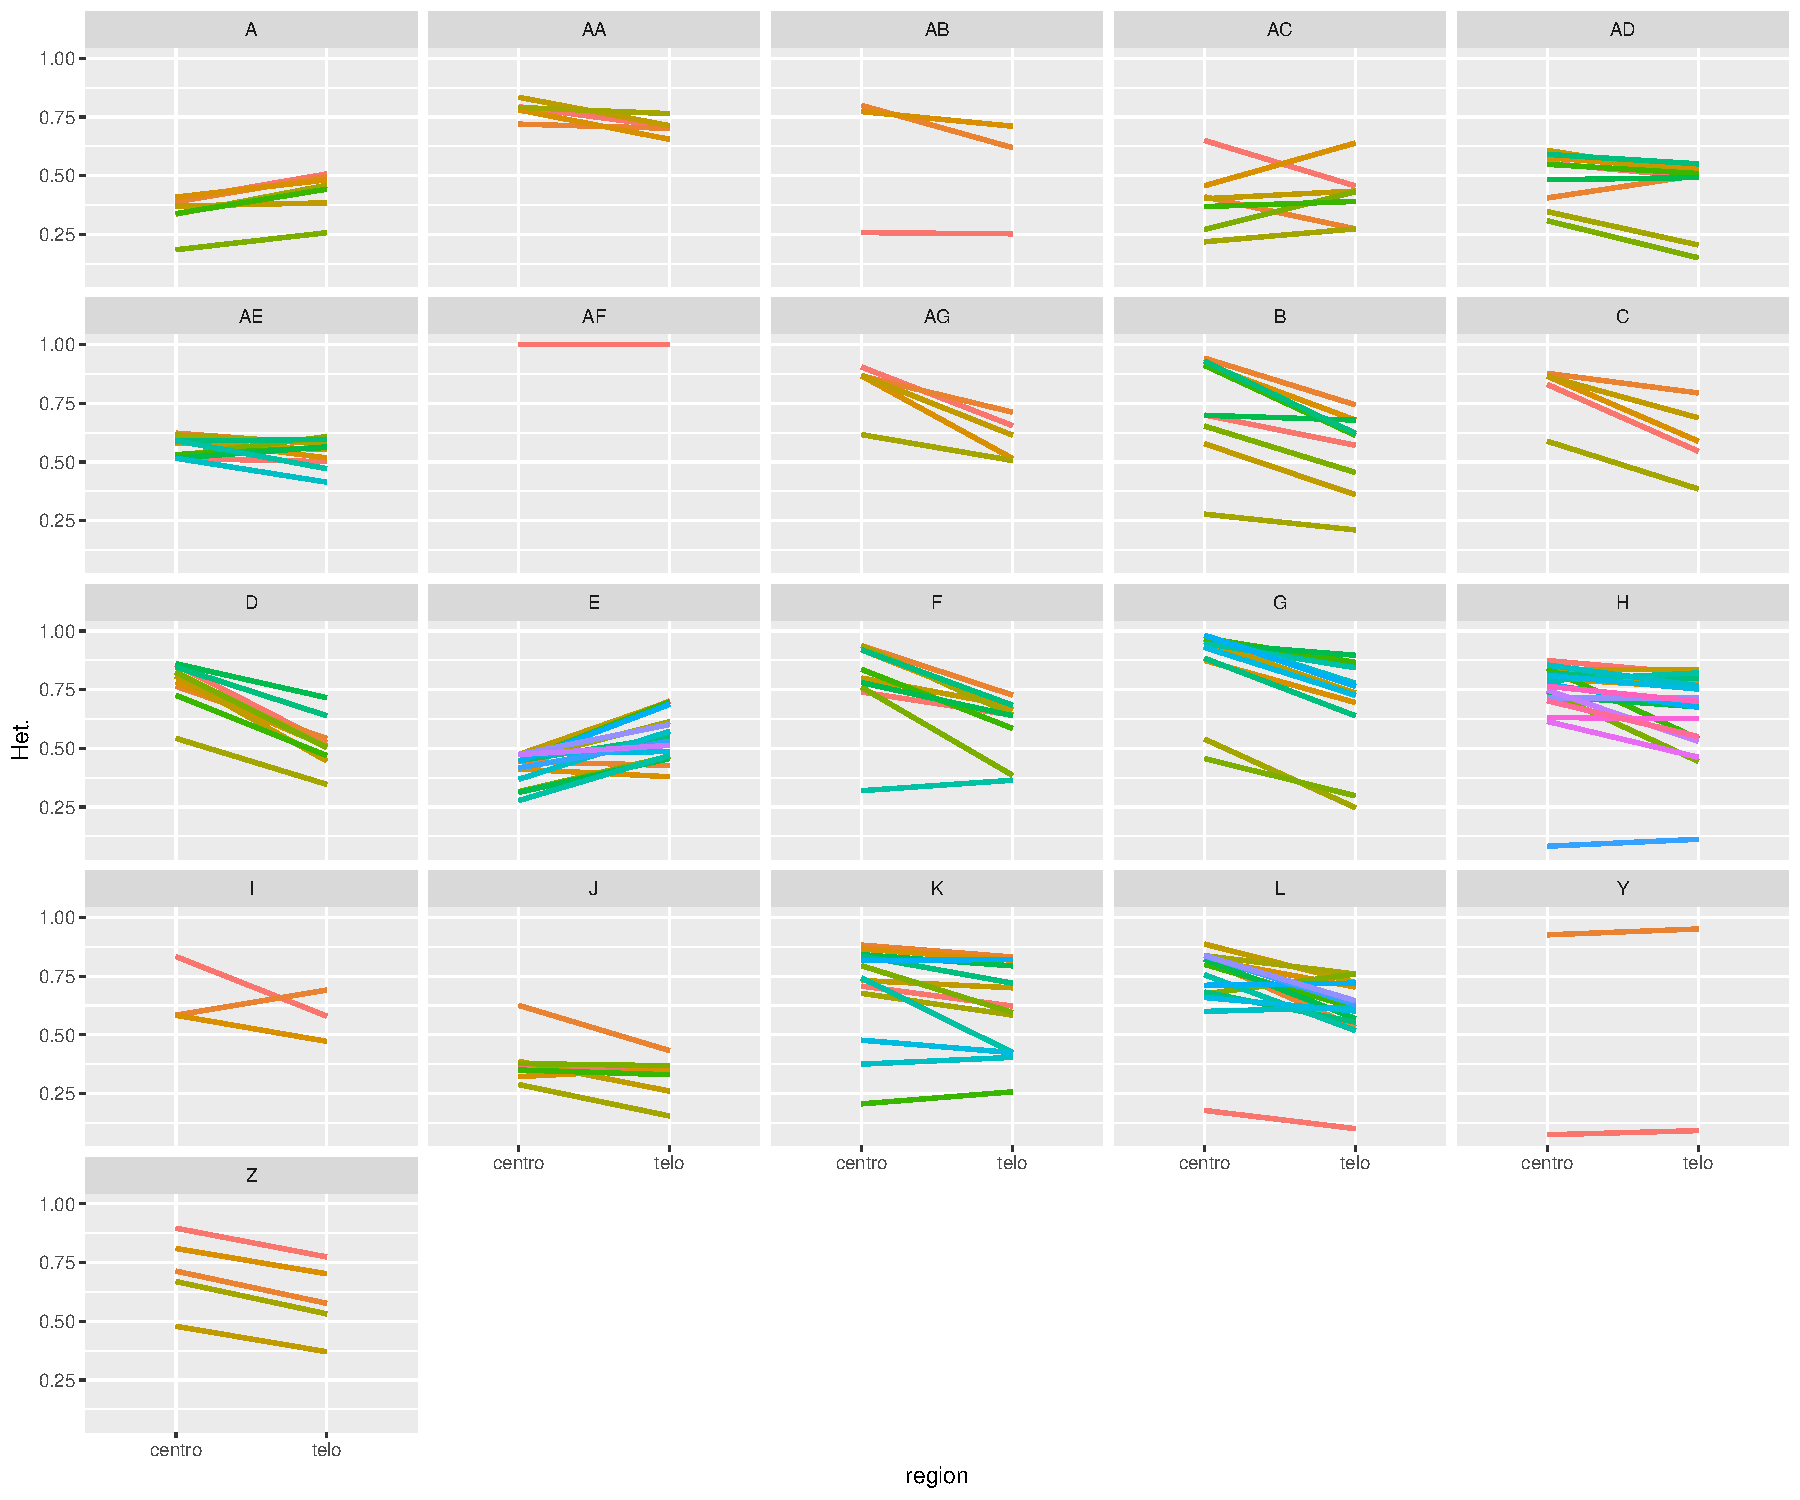
\includegraphics[width=1\textwidth]{Num_CSD_loci/lm_centro25_telo_fam.pdf}
		\caption{Comparing the proportion of heterozygous SNPs pooling all chromosomes together, between the centromeric window (SNPs closer than 25\% of maximum distance to centromere) and telomeric window (SNPs further than 75\%). A linear model is performed to compare the 2 windows and the value of each chromosome is weighted by the number of SNPs used to compute the window.}
		\label{cen_tel_lm}
	\end{center}
\end{figure}

\FloatBarrier

\chapter{Male-Female Fst}

Date: 17.07.2017\\
During preliminary analyses, I noticed recurrent peaks in Fst between diploid males and females in different families. This could indicate the presence of male-deleterious alleles. To further investigate this possibility, I analysed Fst again using all individuals (including haploids).

I first looked at Fst over all 6 chromosomes in the assembly, averaging the Fst at each SNP across family to have an overview (Figure \ref{haplo_Fst_avg}), and then splitting the families to identify recurrent peaks (Figure \ref{haplo_Fst_per_fam}).

\begin{figure}[h]
	\begin{center}
		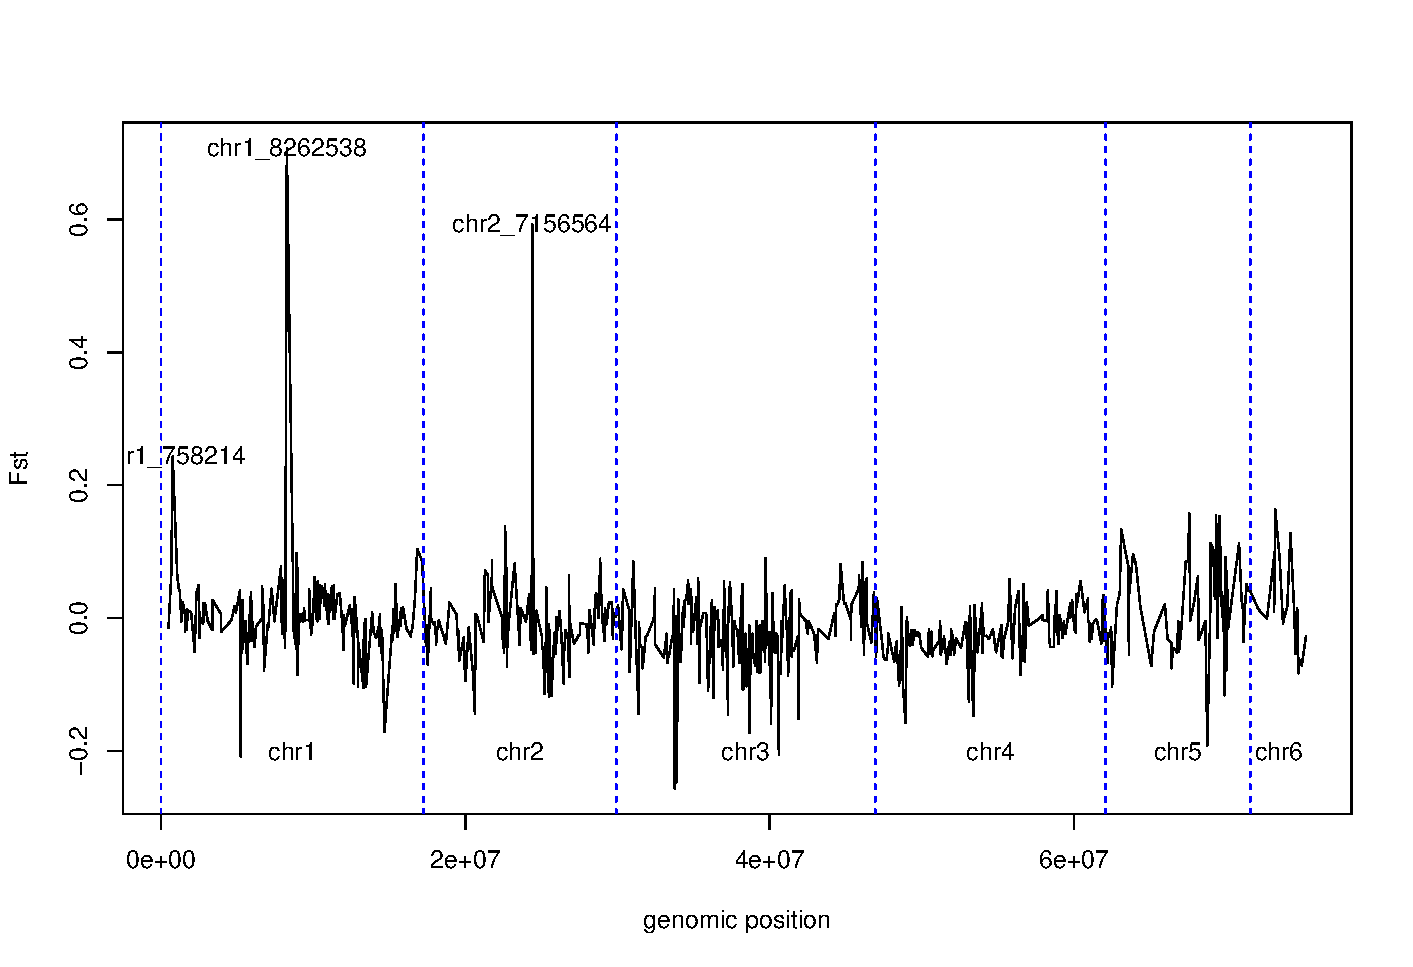
\includegraphics[width=0.8\textwidth]{M-F_Fst/haplo_avg_all_Fst.pdf}
		\caption{Fst values averaged at each SNP across all families. All individuals, including haploids and mothers are included in the analysis and top scoring peaks are labelled with the SNP position in the format "chromosome\_basepair" where basepair is the position within the chromosome. Note: populations parameters set to : min depth (D)=20 and prop pop (r)=80}
		\label{haplo_Fst_avg}
	\end{center}
\end{figure}

\begin{figure}[h]
	\begin{center}
		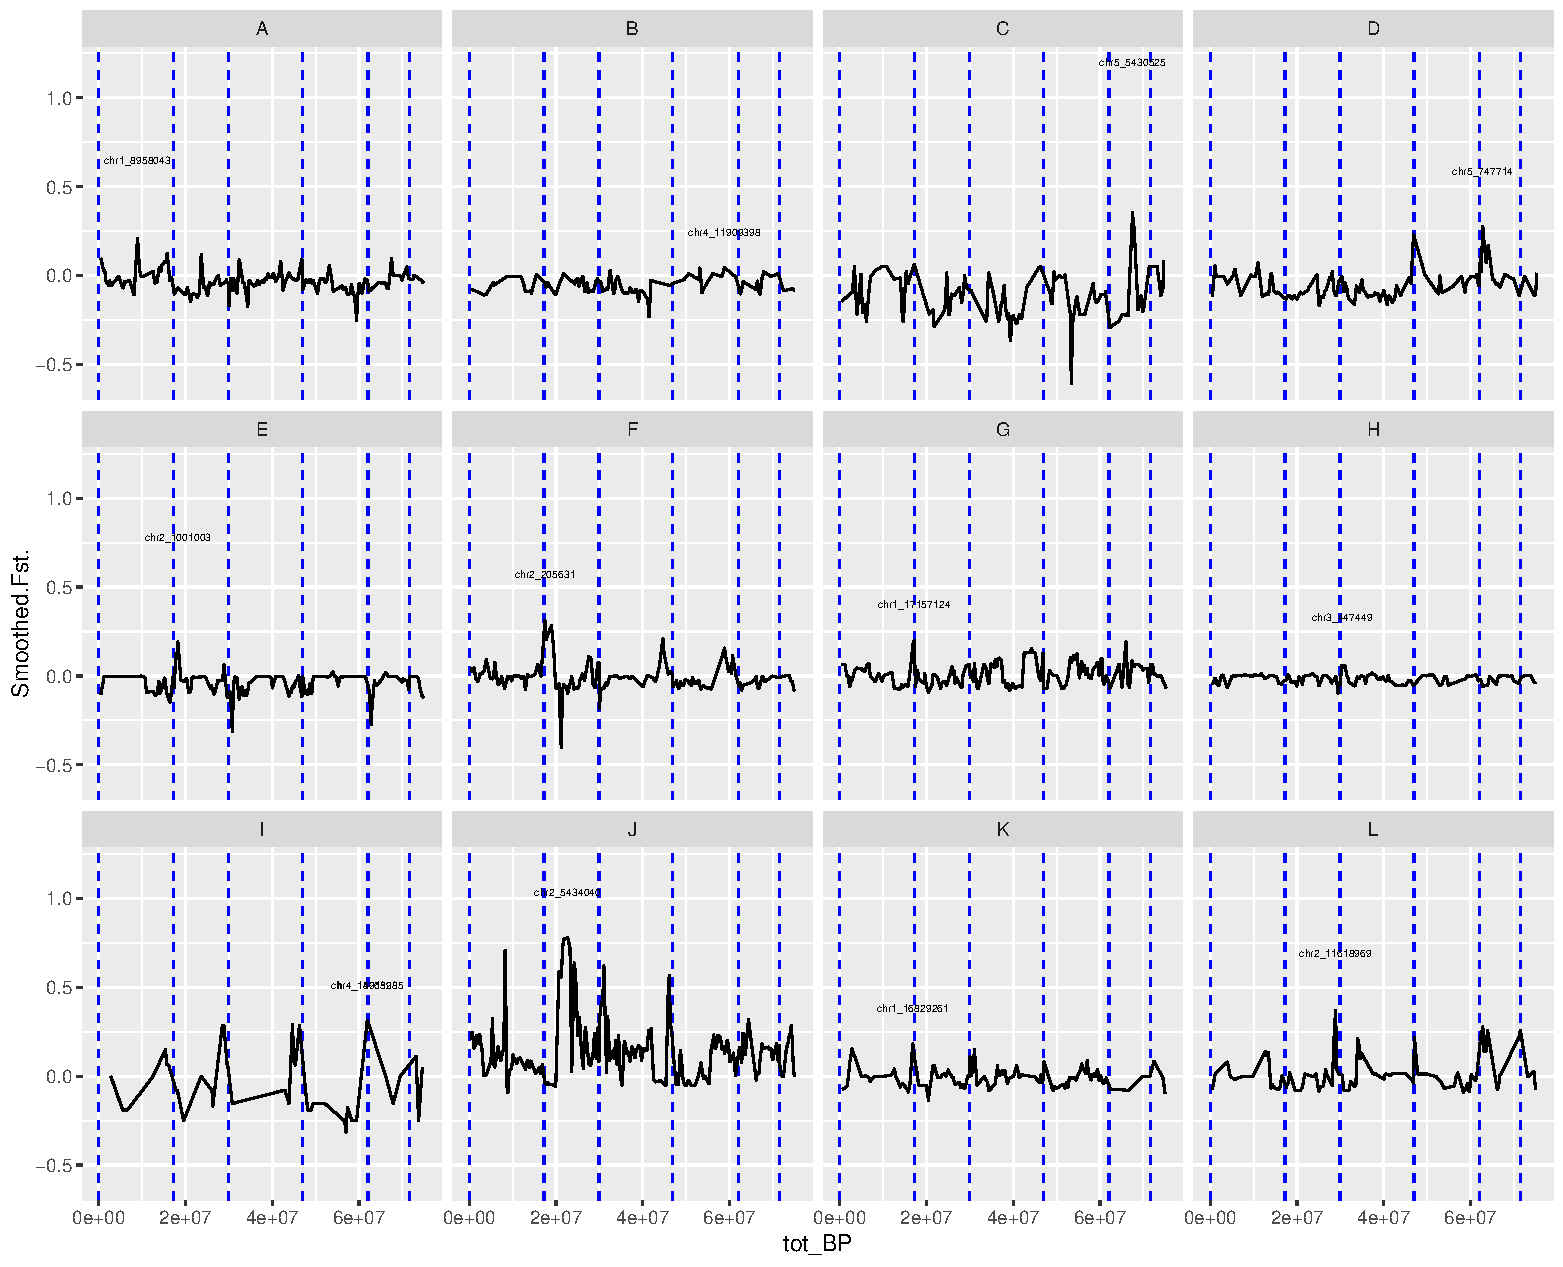
\includegraphics[width=\textwidth]{M-F_Fst/haplo_Fst_per_fam.pdf}
		\caption{Fst values at each SNP by family. All individuals, including haploids and mothers are included in the analysis and top scoring peaks are labelled with the SNP position in the format "chromosome\_basepair" where basepair is the position within the chromosome. Note: populations parameters set to : min depth (D)=20 and prop pop (r)=80}
		\label{haplo_Fst_per_fam}
	\end{center}
\end{figure}
\FloatBarrier

The issue with averaging the Fst over families as in figure \ref{haplo_Fst_avg} is that some SNPs can be sequenced in only one family, therefore the averaged value will only depend on that family. If we merge all families' curve into a single plot, it appears there is no single peak common to all families. 
This can either mean that there is no interesting signal, or if that the signal depends on the family's genetic background, possibly due to an epistatic effect. Here, however, I do not have the sample size to test for it. 

This issue will be dropped from the analysis as the effect is much weaker than what we expected at first and probably just random noise.

\chapter{Association mapping}

\section{Coarse analyses}
Before running any association mapping analysis, I will scan the genome for region that are frequently homozygous in males and heterozygous in females. This is done only after removing SNPs that are homozygous in mothers and individuals that are defined as haploids with fixed homozygosity threshold from the populations analysis.\\

Date: 21.08.2017

The statistic I use when scanning the genome for CSD is $CSD=\frac{Hom_m+Het_f}{2}$ where $Hom_m$ and $Het_f$ are the proportions of homozygous males and heterozygous females respectively at each SNP. If the value is 1, all individuals respect the CSD pattern (all males are homozygous and all females are heterozygous) if it is 0, no individuals respect it (all males are heterozygous and all females homozygous). This metric should not be biased by the gradual decrease in heterozygosity along the chromosome arms as the same weight is given to males and females regardless of numbers. 

\section{Case-control association test}

Date: 18.08.2017
I will use a simple case-control odds ratio to identify CSD hits. I will first do it without taking families into account. I will then perform this test separately for each category of mother and finally I will use distance to centromeres to refine the lists of hits (c.f. Chapter: \ref{sec:num_csd} Number of CSD loci").

The odds ratio are computed fo each SNP using the following observed (O) contingency table where each cell is the number of genotypes corresponding to the category:

\begin{table}[h!]
\begin{tabular}{c|c c c}
& Homozygous & Heterozygous & Total\\
\hline
Male & Mo & Me & Mt\\
Female & Fo & Fe & Ft\\
Total & To & Te & Tt\\
\vspace{5px}
\end{tabular}
\end{table}

Accordingly, the expected  (E) numbers are given by:

\begin{table}[h!]
\begin{tabular}{c|c c c}
& Homozygous & Heterozygous & Total\\[5px]
\hline\\[5px]
Male & $\frac{Mt*To)}{Tt}$ & $\frac{Mt*Te)}{Tt}$ & Mt\\[5px]
Female & $\frac{Ft*To)}{Tt}$ & $\frac{Ft*Te)}{Tt}$ & Ft\\[5px]
Total & To & Te & Tt\\
\vspace{5px}
\end{tabular}
\end{table}

The $\chi^2$ can then be measured as follows:\\
$\chi^2= \frac{(O(Mo)-E(Mo))^2}{E(Mo)} + \frac{(O(Me)-E(Me))^2}{E(Me)} + \frac{(O(Fo)-E(Fo))^2}{E(Fo)} + \frac{(O(Fe)-E(Fe))^2}{E(Fe)}$

I applied this approach on grouped (i.e. single population run with all families) pooled (proportion of homozygous individuals calculated using all families for each SNP) data to have a first insight on the potentially interesting regions (Figure \ref{naive_case_control}). If I want to get reliable results however, I will need to use a different association mapping technique that takes family information into account and to perform the test separately on each category of family (see section: \ref{sec:cat_mothers}, "Categorizing mothers").

\begin{figure}[h]
	\begin{center}
		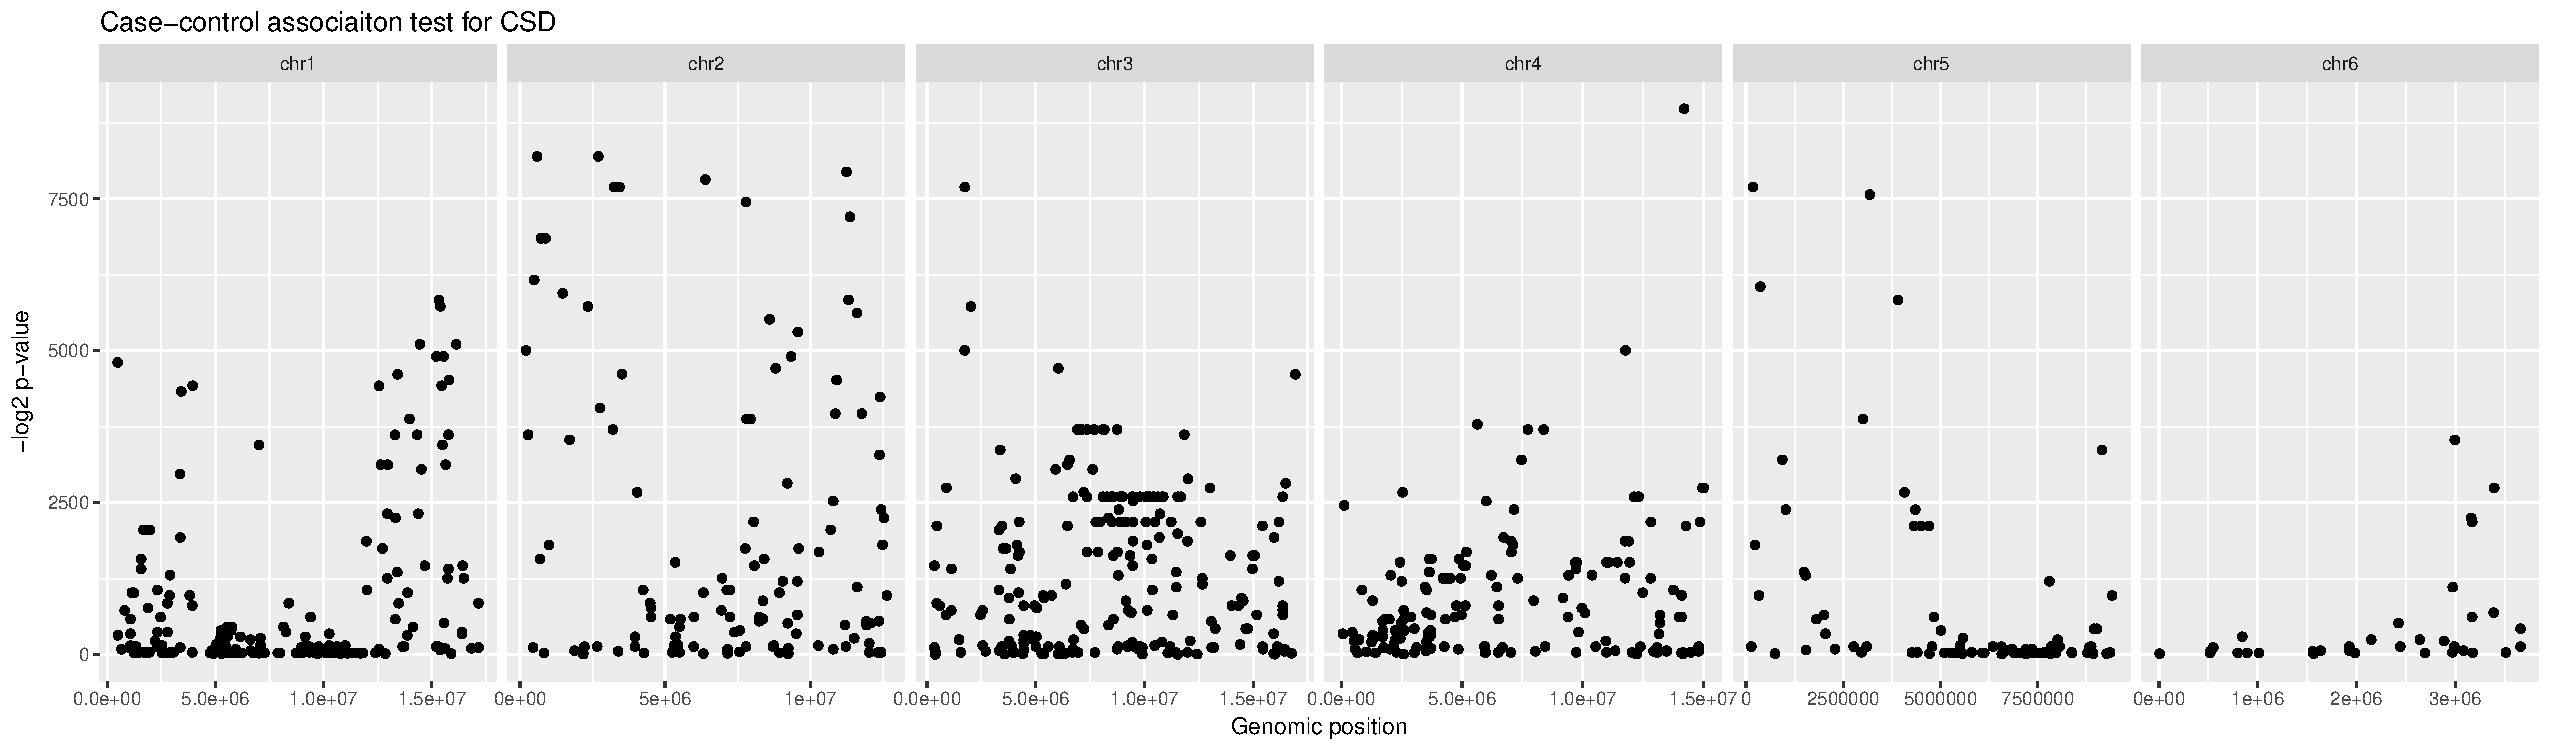
\includegraphics[width=\textwidth]{association_mapping/naive_case_control_grouped.pdf}
		\caption{Manhattan plots with log2 p-values for the case-control association test on CSD. Populations was run on all families together and for each SNP, all individuals were pooled to compute the proportion of homozygous individuals}
		\label{naive_case_control}
	\end{center}
\end{figure}

Date: 31.08.2017\\
The chi2 test is not appropriate in this case especially since I have small values in my cells, I will use Fisher-exact test instead.\\
Date: 01.09.2017\\
Using association mapping with the Fisher-exact test and pooling new indiviudals (including those from library 10b) together yields a few candidate regions and seems promising (Figure \ref{assoc_fisher}). I tried it both with the Benjamini-Hochberg correction (Figure \ref{fisher_BH}) and the bonferroni correction (Figure \ref{fisher_bonferroni}). The next step will be to perform this association mapping per category and to identify the genes in the candidate regions.

\begin{figure}[h]
	\begin{center}
		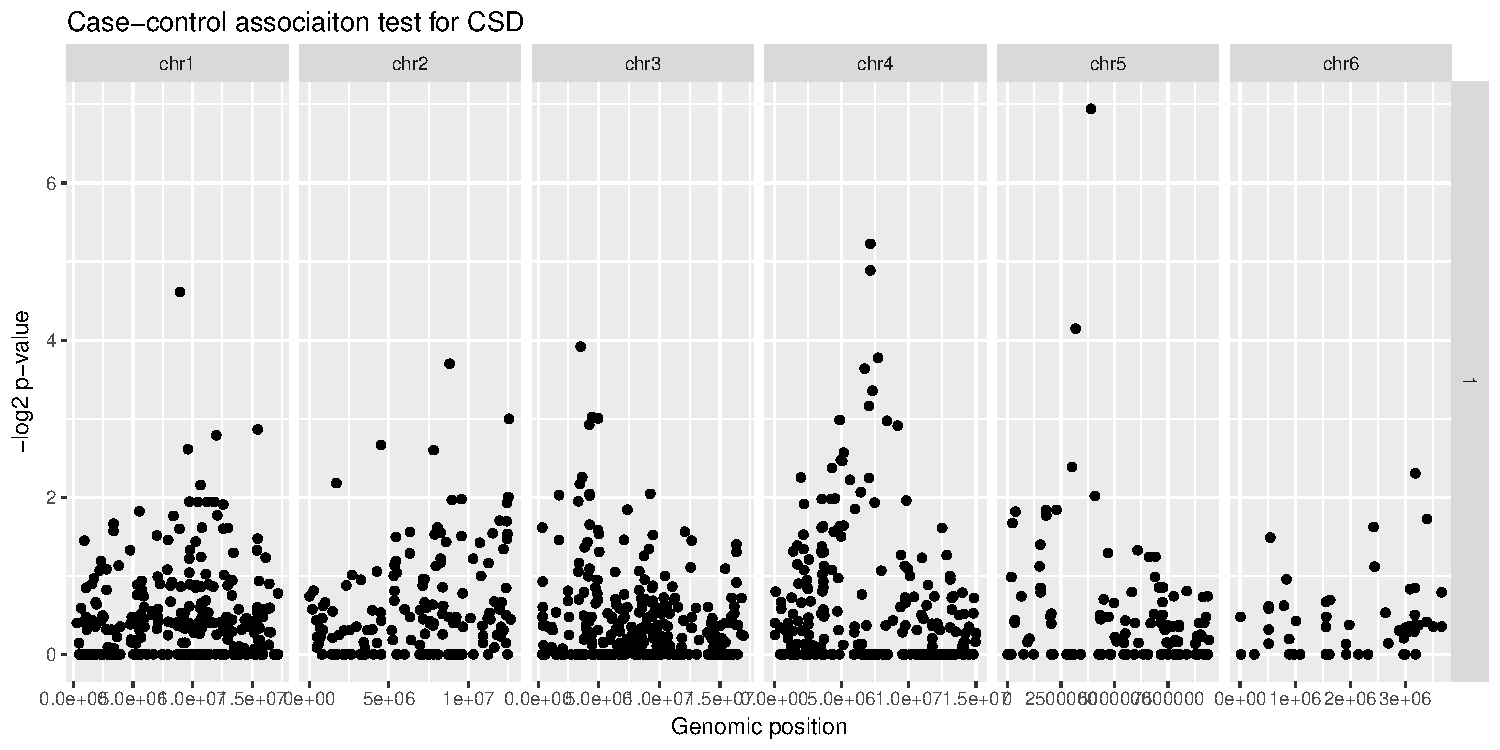
\includegraphics[width=\textwidth]{association_mapping/fisher_no_corr.pdf}
		\caption{Manhattan plots with log10 p-values for the case-control association test on CSD using Fisher exact test. Populations was run on all families together and for each SNP, all individuals were pooled to compute the proportion of homozygous individuals. P-values are not corrected for multiple testing. P-value thresholds of 0.05 and 0.01 are displayed using horizontal black and red lines respectively.}
		\label{assoc_fisher}
	\end{center}
\end{figure}

\begin{figure}[h]
	\begin{center}
		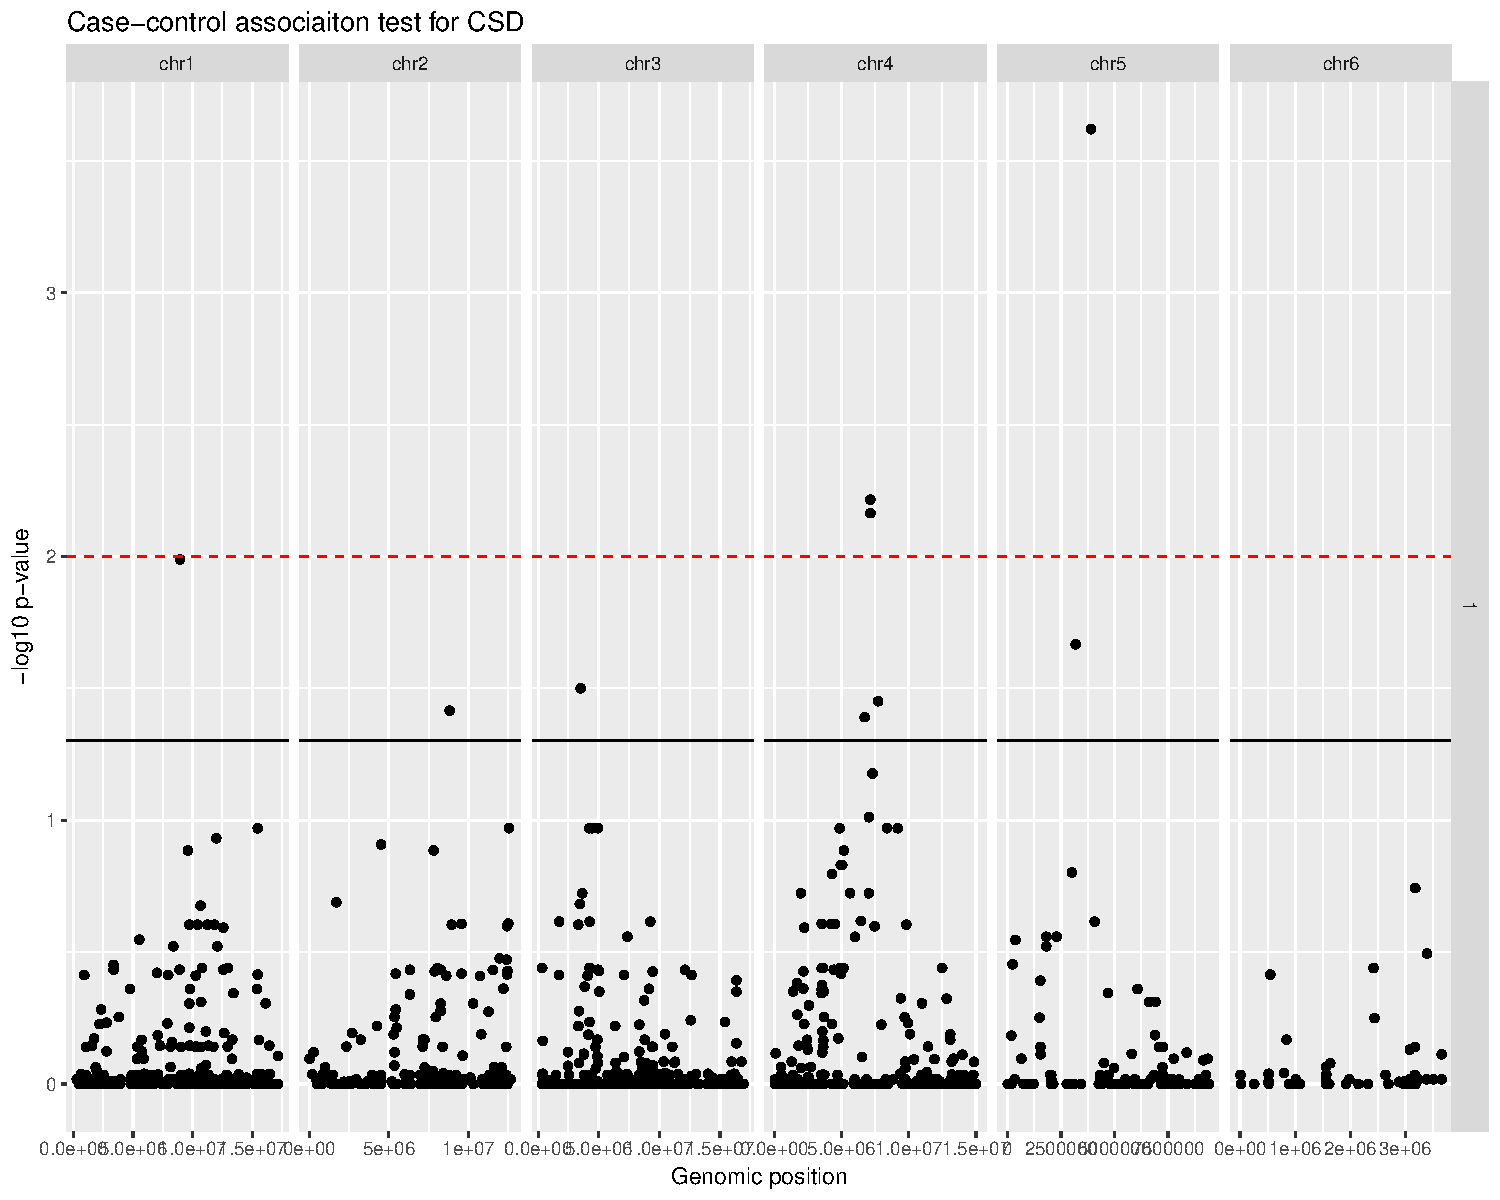
\includegraphics[width=\textwidth]{association_mapping/fisher_BH.pdf}
		\caption{Manhattan plots with log10 p-values for the case-control association test on CSD using Fisher exact test. Populations was run on all families together and for each SNP, all individuals were pooled to compute the proportion of homozygous individuals. Benjamini-Hochberg correction for multiple testing was applied. P-value thresholds of 0.05 and 0.01 are displayed using horizontal black and red lines respectively.}
		\label{fisher_BH}
	\end{center}
\end{figure}

\begin{figure}[h]
	\begin{center}
		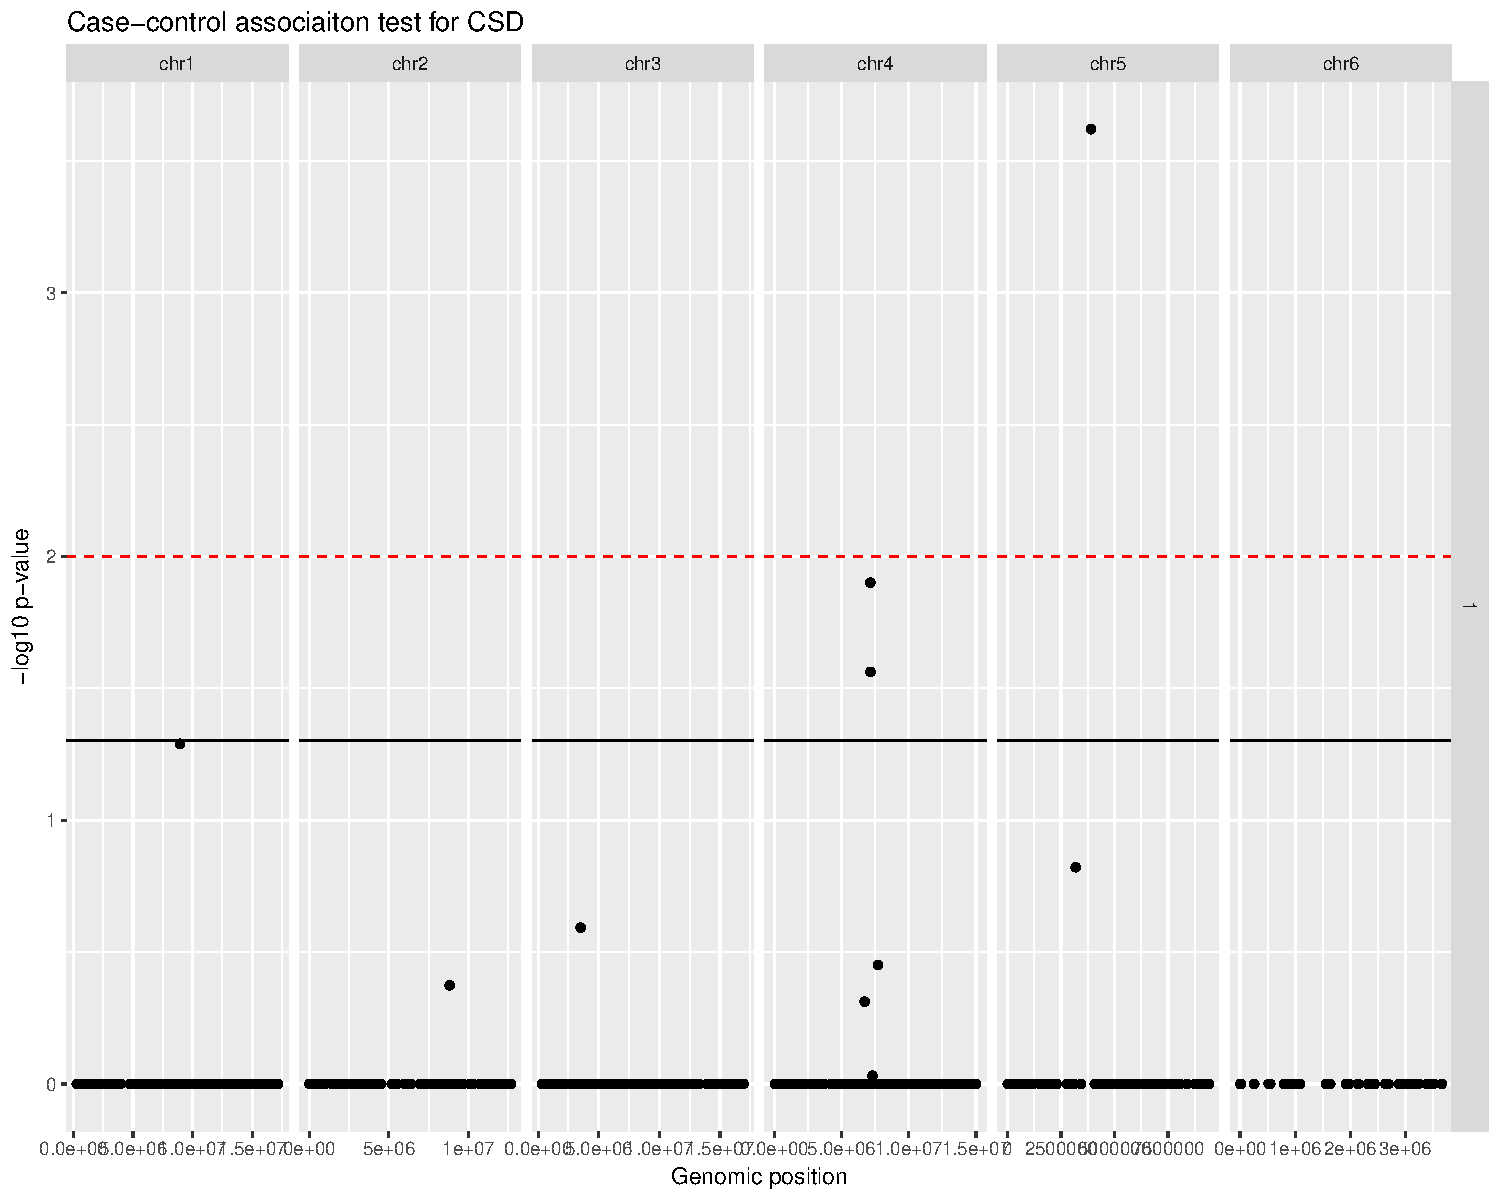
\includegraphics[width=\textwidth]{association_mapping/fisher_bonferroni.pdf}
		\caption{Manhattan plots with log10 p-values for the case-control association test on CSD using Fisher exact test. Populations was run on all families together and for each SNP, all individuals were pooled to compute the proportion of homozygous individuals. Bonferroni correction for multiple testing was applied. P-value thresholds of 0.05 and 0.01 are displayed using horizontal black and red lines respectively.}
		\label{fisher_bonferroni}
	\end{center}
\end{figure}

\subsection{Case-control on categories}

Here, I apply the test after subsetting individuals by categories, inferred using diploid male production as detailed in section \ref{sec:cat_mothers} "Categorizing mothers". 

I will do it considering different number of categories, corresponding to different scenarios regarding the number of CSD loci. Figure \ref{naive_case_control} already addresses the unlikely scenario of single-locus CSD. Here, I will deal with 2 and 3 loci scenarios, with 3 and 7 categories, respectively.

\subsection{Refining hits using centromeres}


\section{Family-based association mapping}

I will try to adapt the "generalized family-based association test for dichotomous traits" (GDT) published by Chen W.-M., Manichaikul A. and Rich S.S. in The American Journal of Human Genetics (2009). This test should work both in inbred and non-inbred families and takes family information into account.\\

Here, I will modify the test presented in the publication to test for association of homozygosity with male phenotype instead of a particular allele with a disease. I will also need to make it work with a single parent.

Date 23.08.2017

After investigating the proofs of the score used in the family based test mentioned above, I realized adapting it would not make sense; it uses pedigree information and relies on the differences in kinship coefficients or proportion of IBD alleles. Since I have asexuals, all kinship coefficient in the families are 1, they are all siblings and it does not make much sense to include pedigree information. 
I will instead focus on a better implementation of the case-control test.

\chapter{Coverage analysis}

In this section, I check wether there are individuals or genomic regions that have abnormally high or low coverage, I identify the potential reasons for these abnormalities and eventually, I will remove the concerned elements from the analysis.

\section{Individual stats}

Prior to coverage, I had a look at the raw reads statistics. On average,each sample has 803951 reads and the (ordered) reference genome is 140.7 Mb long. This makes for an average of $5.7*10^{-3}$ reads per basepair.
In comparison, the 3 datasets used in the Paris 2017 paper (Roadmap to STACKS) have $9.6*10^{-4}$, $2.7*10^{-3}$ and $8.6*10^{-3}$.

I first analysed the coverage on a per individual basis. That means for each individual, it has been averaged over all polymorphic SNPs kept throughout the STACKS pipeline. The mean sample coverage is relatively high and follows a normal distribution centered around 119X with a standard deviation of 33. There are two outliers with exceptionally high coverage (at 228X and 270X, respectively) which I might consider removing. The coverage is not different across families (Figure \ref{cov_fam}). Coverage is not affected by the family of an individual (it is not affected by ploidy or sex either).

\begin{figure}[h]
	\begin{center}
		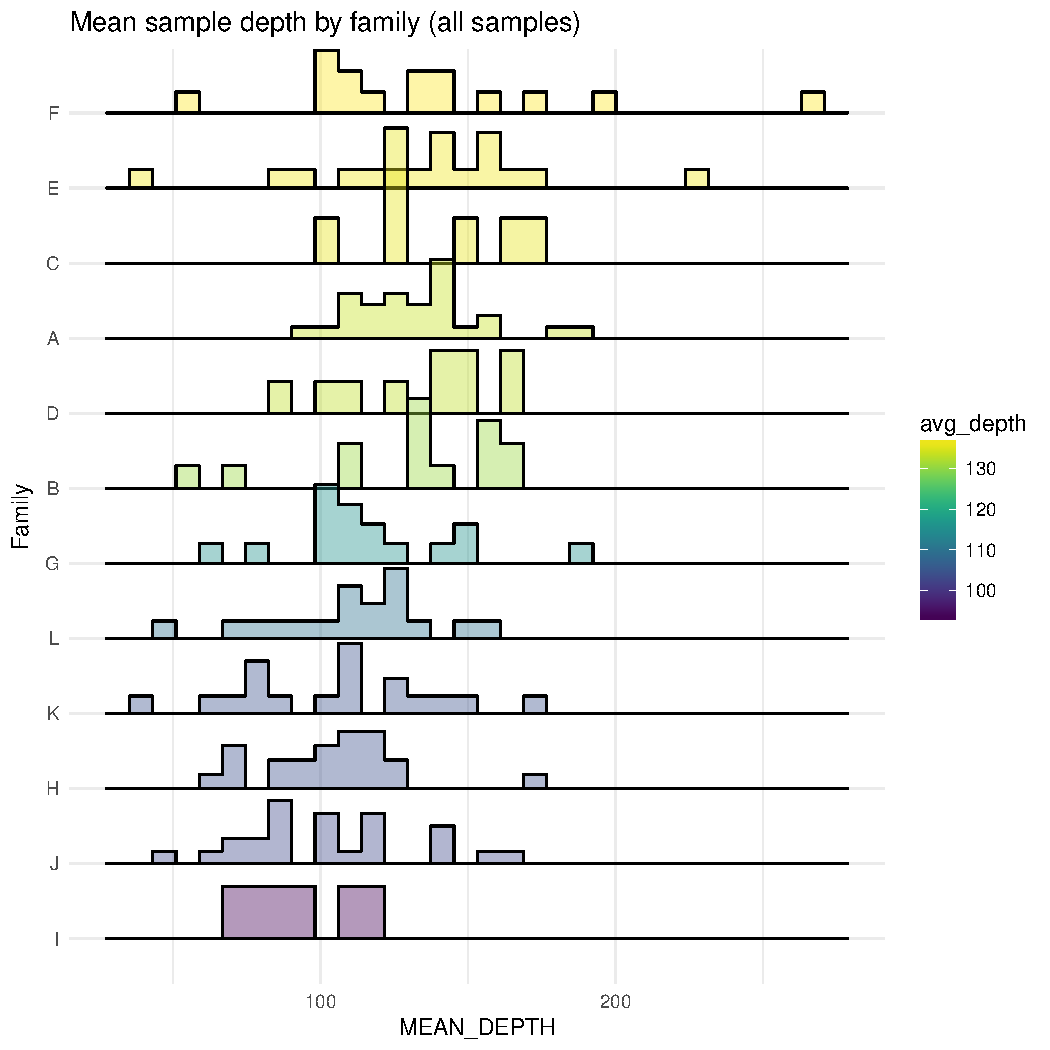
\includegraphics[width=0.70\textwidth]{coverage_analysis/cov_per_sample.pdf}
		\caption{Sample depth, averaged across all polymorphic sites which passed STACKS populations filters. Individuals of each family are plotted together and histograms are colored according to the family's mean depth.}
		\label{sites_fam}
	\end{center}
\end{figure}

Analyzing the number of sites (SNPs) per sample revealed that it was strongly affected by the family (Figure \ref{sites_fam}). This could be caused by storage duration, reagent quality or manipulations. If so, I cannot account for this and will either need to get rid of lowest quality families (such as I) or get more individuals.\\

Update: 06.08.2017

To investigate whether the inter-family variation in the number of sequenced sites was due to differing amounts of sequenced DNA, I compared the number of sequencing reads per family (Figure \ref{reads_fam}). There is interfamily variation, but it seems relatively low, compared to the number of sites in figure \ref{sites_fam}. This variation is likely due to the low number of samples and is probably not meaningful. Moreover, the order of families, when sorted from highest to lowest is different for number of sequenced sites and number of reads. 



\begin{figure}[h]
	\begin{center}
		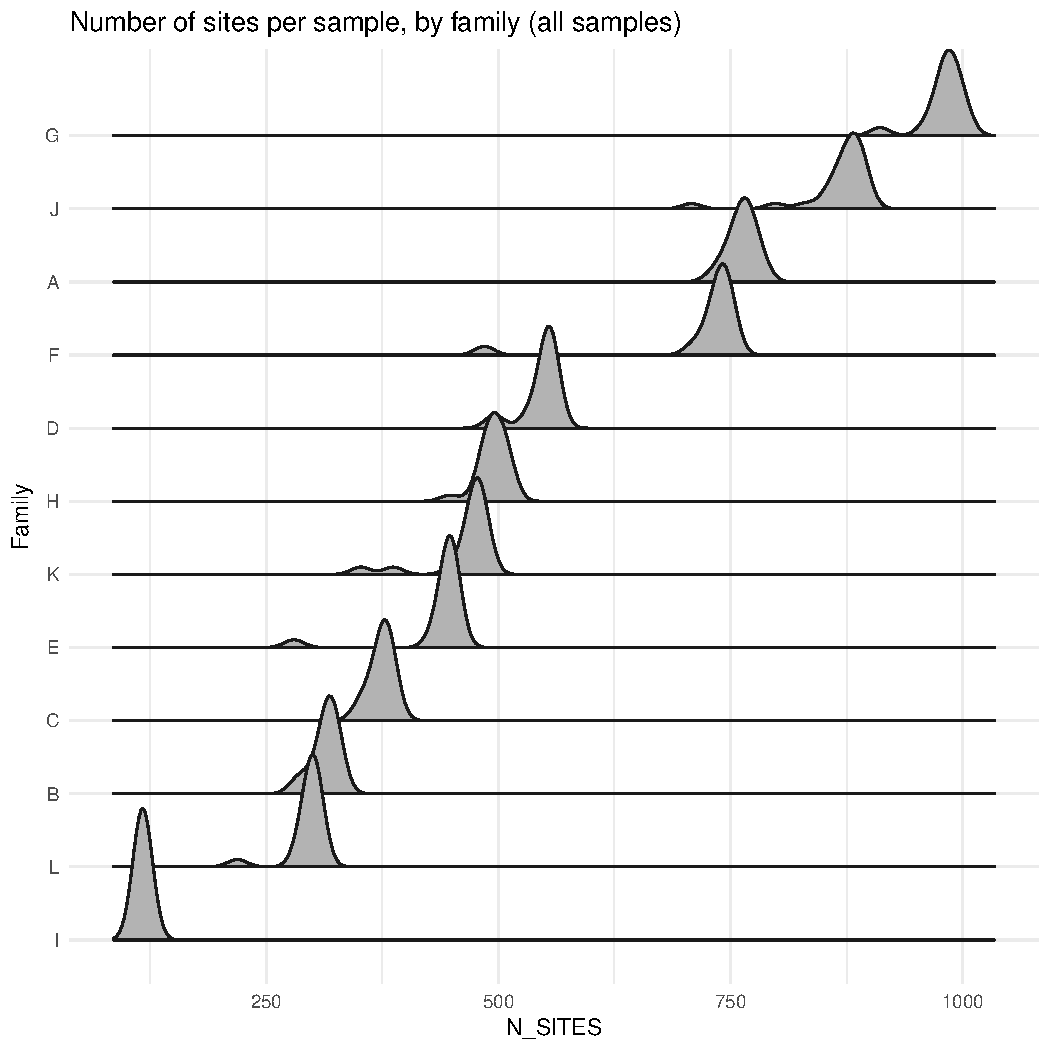
\includegraphics[width=0.7\textwidth]{coverage_analysis/sites_per_sample.pdf}
		\caption{Number of polymorphic sites (SNPs) per individual that passed the STACKS populations filters. Distribution of individuals is shown by family. There is a strong clustering of families.}
		\label{sites_fam}
	\end{center}
\end{figure}


\begin{figure}[h]
	\begin{center}
		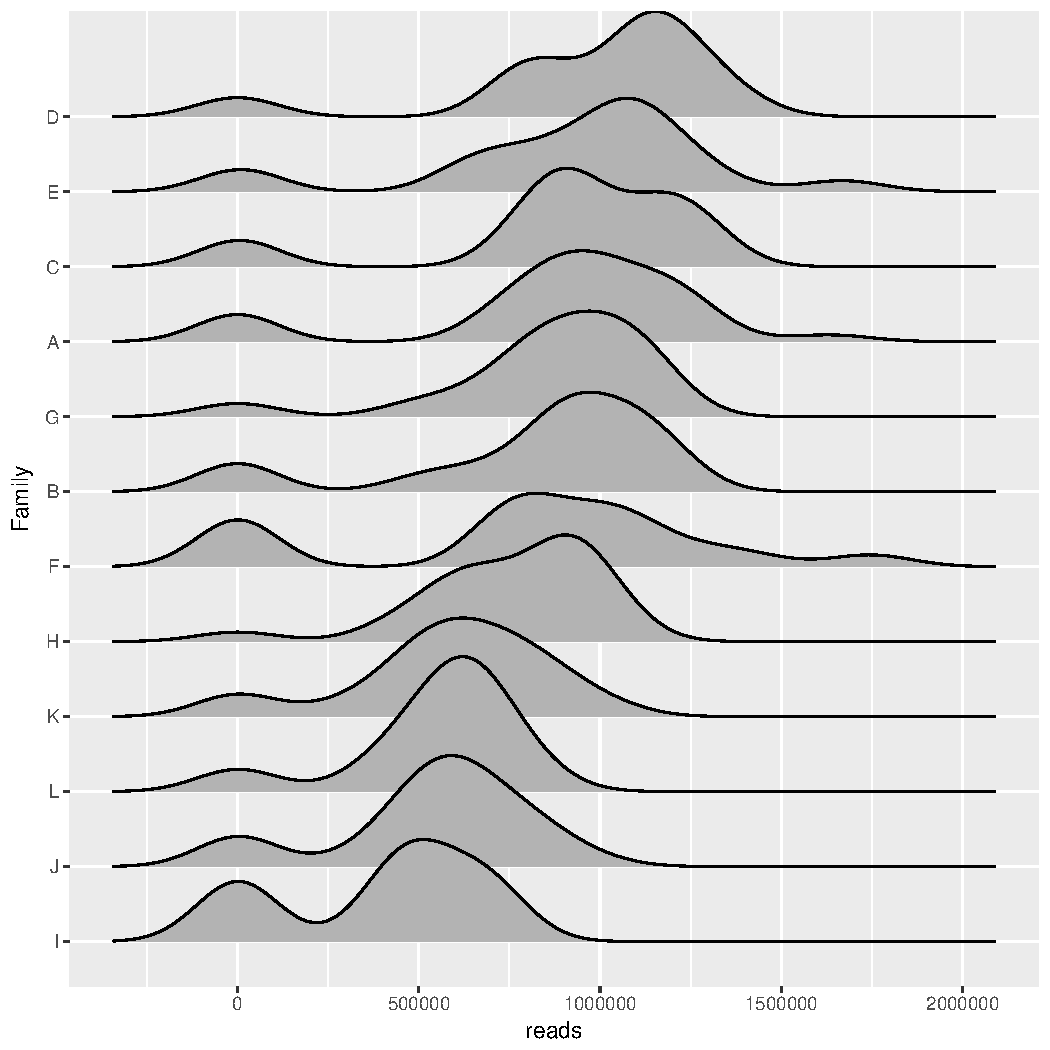
\includegraphics[width=0.7\textwidth]{coverage_analysis/reads_sample.pdf}
		\caption{Number of sequencing reads per individual, before mapping or any filter. Distribution of individuals is shown by family. The inter-family variation is not particularly high relative to intra-family variation.}
		\label{reads_fam}
	\end{center}
\end{figure}


\section{Genome coverage}

To identify regions of high or low coverage, I extracted information about the mean coverage per family at each polymorphic site that passed the STACKS populations filters. I then binned SNPs by 1kb regions (Figure \ref{cov_genome}).
Some SNPs have extreme coverage values (>600X) and might be caused by repetitive regions or paralogs that have been merged as a single locus.

\begin{figure}[h]
	\begin{center}
		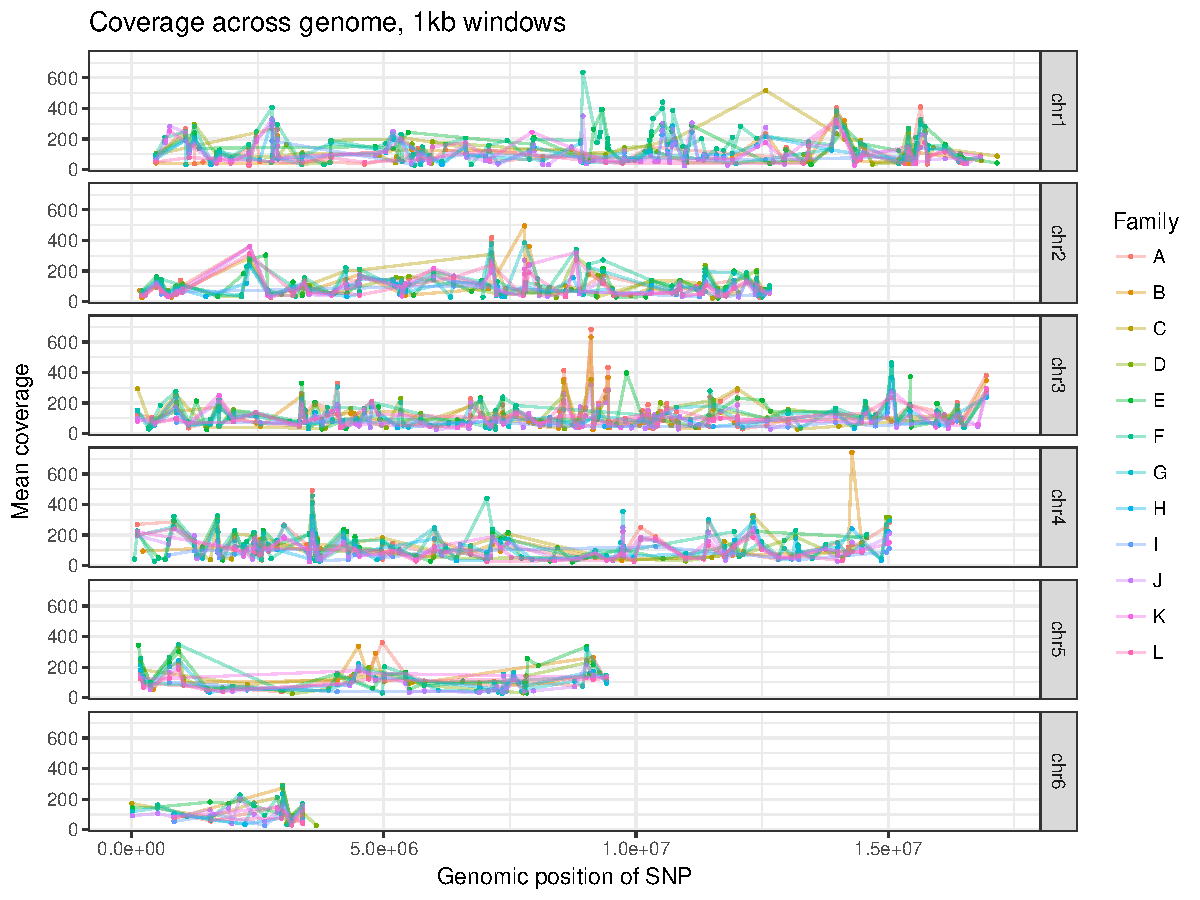
\includegraphics[width=\textwidth]{coverage_analysis/coverage_1kbwin.pdf}
		\caption{Mean depth per family at every SNP that passed the populations filters.}
		\label{cov_genome}
	\end{center}
\end{figure}

\section{Lowering the filters}

Date: 09.08.2017

The main issues I am facing in this chapter are 1) the abnormally high coverage across my samples and 2) the high variation in the number of sites between families.

The reason the high mean coverage per sample was worrying is because I have about the same amount of reads per sample as the 3 datasets described in the roadmap to stacks paper (Paris et al, 2017), yet i have at least twice more coverage per sample. After re-reading the paper, I found out this was simply a consequence of my stringent filters at the populations stage, which they do not use (see citation below).\\

\textit{"Despite controlling for the mini-
mum read depth of alleles at the ustacks phase of the pipe-
line, many studies also incorporate a minimum stack depth
required for individuals at a locus in the populations mod-
ule of STACKS (e.g. Gaither et al. 2015; Ivy et al. 2016; Kjeldsen
et al. 2016). Such a method is undesirable, as read depth has
already been accounted for by the SNP model. Once the SNP
model has made a determination, its evaluation should be
trusted and using further non-statistically based limits on
depth of coverage is ill advised and will result in the arbitrary
dropping of loci."\\}

I will follow their advice since my coverage is absurdly high, and I would benefit a sharp increase in the number of loci by removing this filter. 

\chapter{Additional samples (lib10 + lib10b)}

Date: 26.08.2017\\
Libraries 10 and 10b got back from the samples and I have processed them through the pipeline. Library10 suffered a dramatic loss in read count due to an unidentified technical problem (~10x less reads than lib10b).\\
IMPORTANT: W10 appeared twice in the name list: once in library 10b and once in what will later be library11. Therefore I shifted the numbering by 1 for family W in library11. I will need to make sure this is the case in the barcode file as well.\\

Date: 28.08.2017\\
After removing all samples from library10 (see subsection \ref{sec:add_coverage} "Coverage", below). I still have NNN diploid individuals, distributed across FFF families.

\section{Data description}
\subsection{Family composition}
With the new samples, I now have 239 diploids across 32 families. Many families are relatively small, however (Figure \ref{off_comp}) and relying on sex ratio among diploid offspring to categorize families could be unreliable.

\begin{figure}[h]
	\begin{center}
		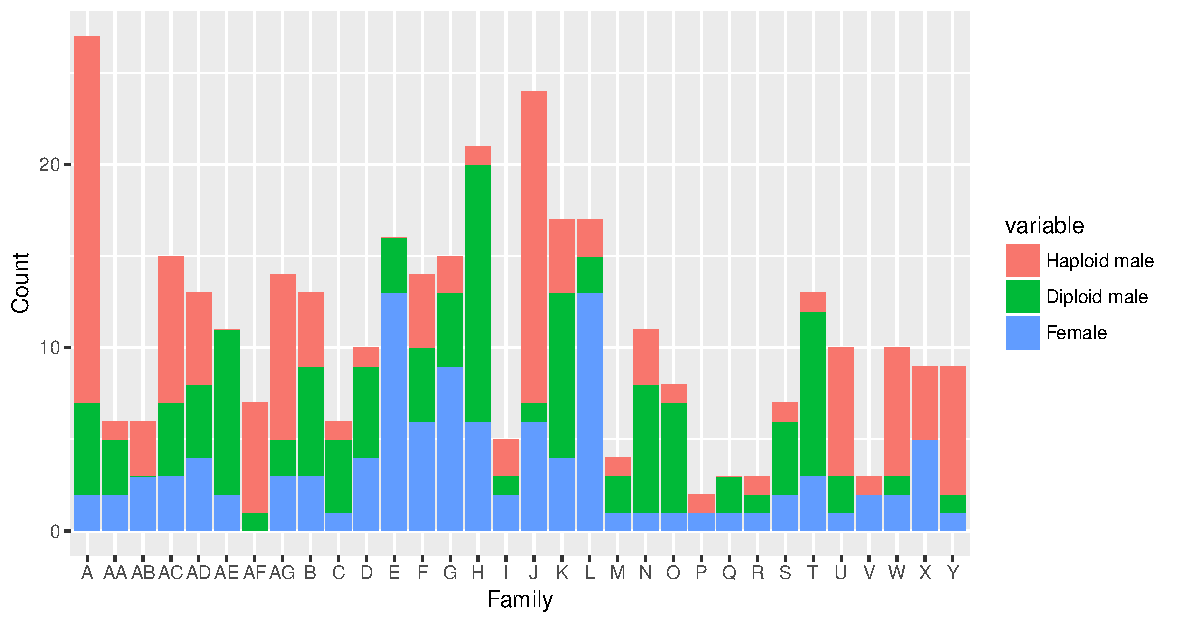
\includegraphics[width=\textwidth]{add_samples/off_comp.pdf}
		\caption{Composition of offspring per family when including new samples from library 10 and 10b.}
		\label{off_comp}
	\end{center}
\end{figure}

\subsection{Coverage}
\label{sec:add_coverage}

The coverage across genome (Figure \ref{cov_genome_add}) did not change much by adding the new libraries, however looking at the coverage per individuals(Figure \ref{mean_depth_add}) and number of site per individuals (Figure \ref{n_sites_add}) confirms the poor quality of library 10. These individuals barely passed the filters i have put in place, but overall they still have very low read counts and including them exposes my whole analysis to technical biases. I will therefore remove all samples from that library. Note that I'll also remove W10 since it is the only healthy sample left in the family and all females are lost (they were in lib10).

\begin{figure}[h]
	\begin{center}
		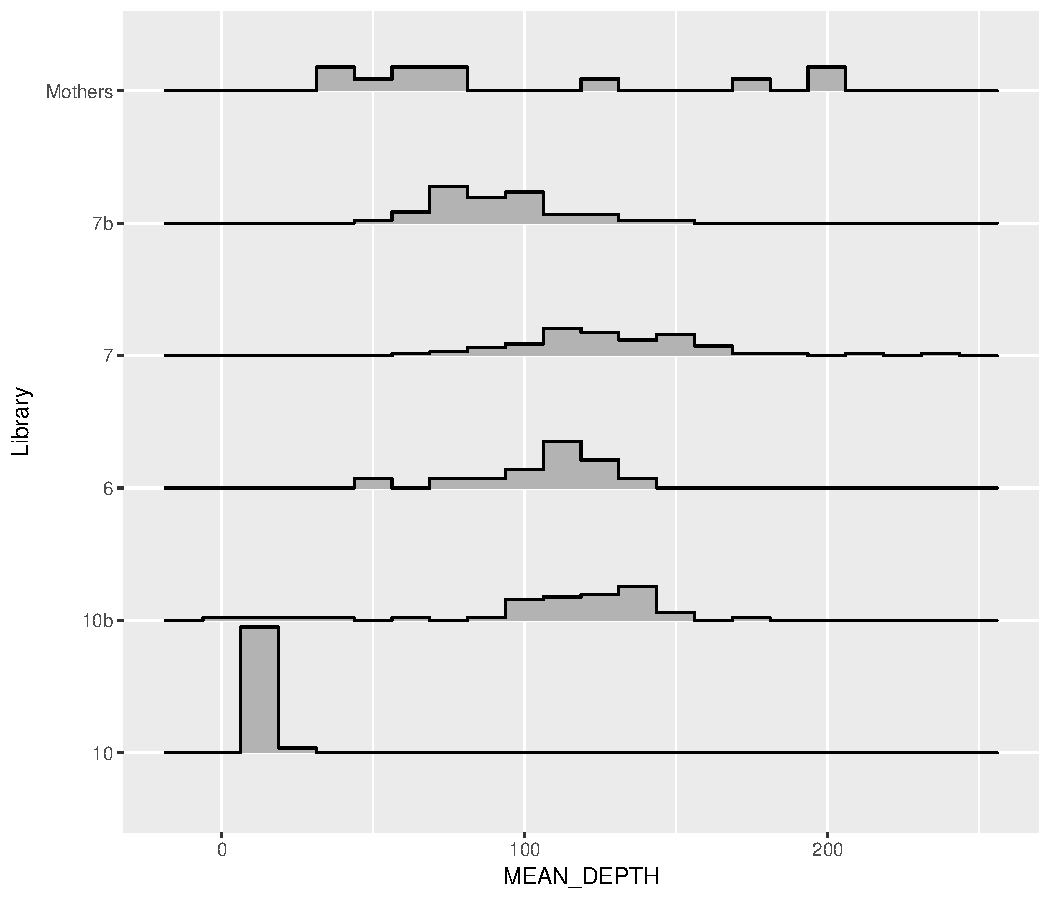
\includegraphics[width=\textwidth]{add_samples/library_depth.pdf}
		\caption{Distribution of the mean sequencing depth per individuals in each library including the new ones (10 and 10b).}
		\label{mean_depth_add}
	\end{center}
\end{figure}

\begin{figure}[h]
	\begin{center}
		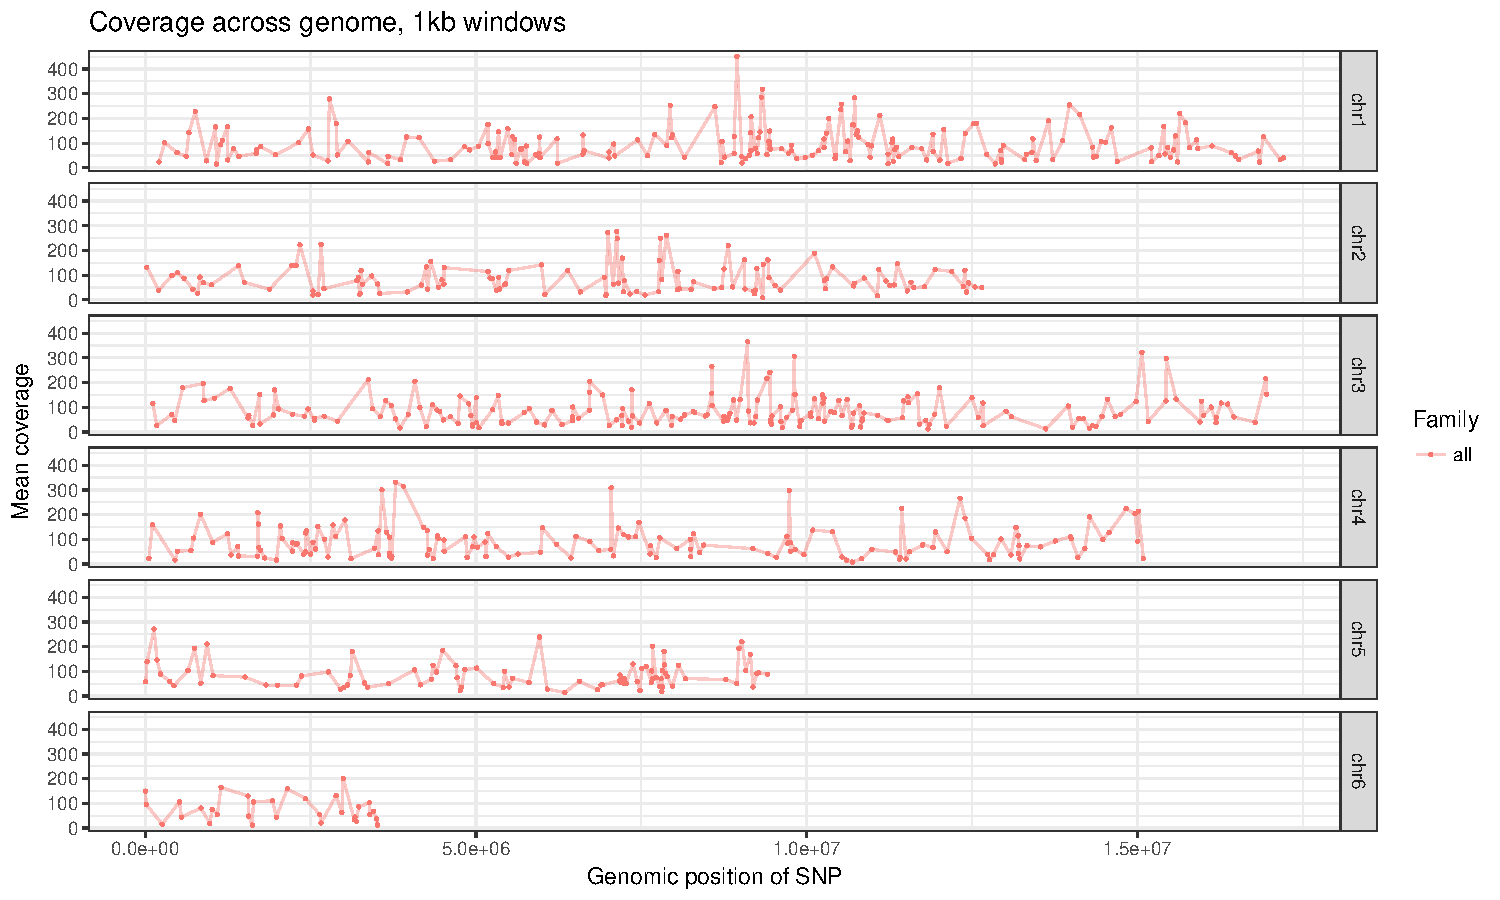
\includegraphics[width=\textwidth]{add_samples/cov_per_site.pdf}
		\caption{Sequencing depth across genome. Depth is averaged over all samples at each sites and values are averaged by 1kb windows. New samples from libraries 10 and 10b are included}
		\label{cov_genome_add}
	\end{center}
\end{figure}

\begin{figure}[h]
	\begin{center}
		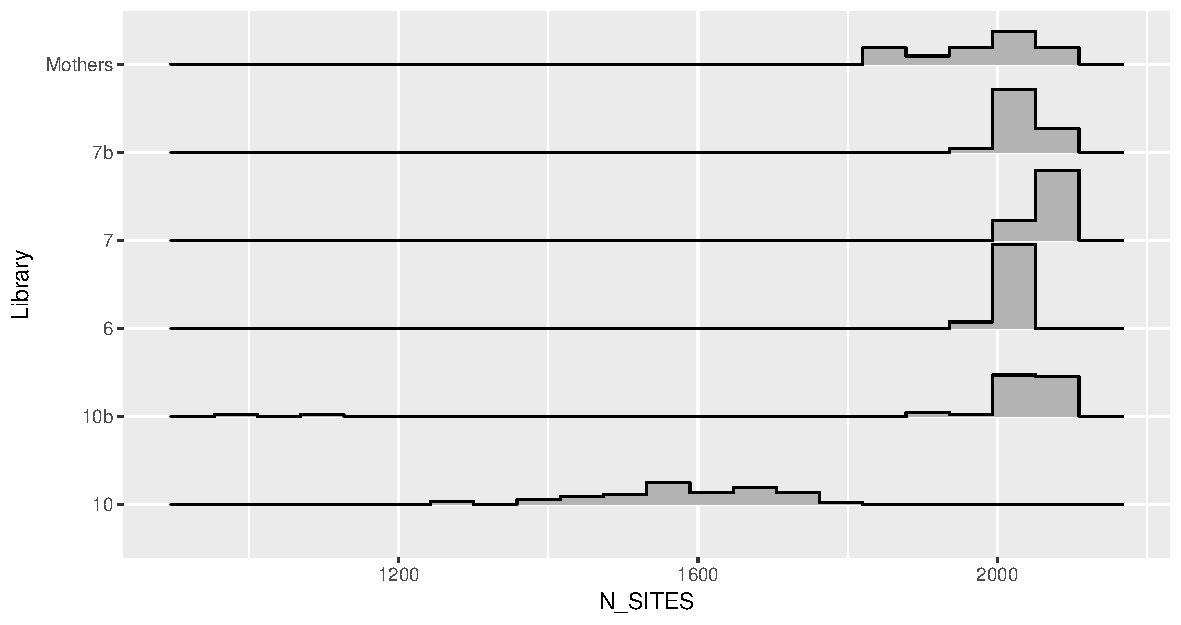
\includegraphics[width=\textwidth]{add_samples/library_sites.pdf}
		\caption{Distribution of the number of sites per individuals in each library including the new ones (10 and 10b).}
		\label{n_sites_add}
	\end{center}
\end{figure}
\FloatBarrier

\section{CSD}

After removing all samples from library 10, I performed the downstream analyses to find CSD again.
\subsection{Grouping mothers}
\subsection{Finding centromeres}
\subsection{CSD scan}
\subsection{Association mapping}

\FloatBarrier
\chapter{TO DO}
\begin{itemize}
\item compute prop.het loci in centromeric window for all individuals and isolate TFA based on distribution if bimodal.
\item try above with different values for window sizes and select based on number of loci contained in window.
\item Compute coverage along genome for all loci including monomorphic ones.
\item Isolate regions of abnodmally high coverage, eventually exclude them. Watch out for overmerging of paralogs and repetitive sequences.
\item Visualize average heterozygosity (or allele frequency) at each SNPs in offpring versus in mother to assess transmission bias (hom SNPs in mothers more often het in offspring or reversse). 
\item Validate haploid definition using haplotypes deduced from linkage map.
\item convert VCF file into PED format using vcftools
\item import data into genABEL and perform association mapping
\item make snp calling less reliant on correct mother calls and exclude SNPs only if mother is hom/missing AND less than N offspring are heterozygous (small N)
\item automate threshold selection for inferring ploidy
\end{itemize}

\end{document} 
\grid
%                                 